\documentclass[a4paper]{scrartcl}

\usepackage[
fancytheorems,
fancyproofs,
noindent,
]{adam}

\usepackage{tikz}
\usepackage{mathtools}

\title{Linear Analysis}
\author{Adam Kelly (\texttt{ak2316@cam.ac.uk})}
\date{\today}

% --- Extra macros for this course ---
\newcommand{\ip}[2]{\langle #1, #2 \rangle}
\newcommand{\spn}{\operatorname{span}}
\newcommand{\Bop}{\mathcal{B}}
\newcommand{\Kop}{\mathcal{K}}
\newcommand{\Hil}{\mathcal{H}}
\newcommand{\wt}{\widetilde}
\newcommand{\id}{\operatorname{id}}
\DeclareMathOperator{\dist}{dist}
\DeclareMathOperator{\diam}{diam}
\DeclareMathOperator{\rank}{rank}
\DeclareMathOperator{\sgn}{sgn}

\allowdisplaybreaks

\begin{document}

\maketitle

Linear analysis is what happens when you take the linear algebra you know and let the dimension become infinite. Almost nothing survives unscathed. A linear map need not be continuous. A subspace need not be closed. A bounded sequence need not have a convergent subsequence, and the closed unit ball -- that most innocuous of objects -- is never compact. The whole edifice of `pick a basis and write down a matrix' collapses, and we need genuinely new tools to replace it.

The tools we get are marvellous. The Hahn--Banach theorem manufactures linear functionals out of thin air, so that a normed space always has a rich supply of them. The Baire category theorem, an almost embarrassingly soft statement about complete metric spaces, yields three of the great theorems of the subject in a single stroke. And in Hilbert space -- where we have not just a length but an angle -- geometry comes flooding back, and we recover a spectral theorem that would make any linear algebraist feel at home.

This article constitutes my notes for the `Linear Analysis' course, held in Michaelmas 2021 at Cambridge. These notes are \emph{not a transcription of the lectures}, and differ significantly in quite a few areas. Still, all lectured material should be covered.

\tableofcontents

\section{Normed Spaces}

Throughout this course, $\F$ will denote either $\R$ or $\C$, and all vector spaces will be over $\F$ unless we say otherwise. When a result works for both fields without change we will just write $\F$; when the distinction matters -- and it does matter, for instance in the Hahn--Banach theorem -- we will be careful to say so.

In IB Linear Algebra we studied vector spaces armed with nothing but their algebraic structure, and for finite-dimensional spaces this was enough: choose a basis, and everything becomes a matrix. In IB Analysis and Topology we studied metric spaces, where we could speak of convergence and continuity but had no algebra to play with. Linear analysis is what you get when you insist on having both at once, in a way that makes them compatible.

\subsection{Norms}

The compatibility is achieved by the following definition, which is really just an abstraction of `length of a vector' in $\R^n$.

\begin{definition}[Norm]
	Let $V$ be a vector space over $\F$. A \vocab{norm} on $V$ is a function $\norm{\cdot} : V \to \R$ such that
	\begin{enumerate}[label=(\roman*)]
		\item (\emph{Positivity}) $\norm{v} \geq 0$ for all $v \in V$, with $\norm{v} = 0$ if and only if $v = 0$;
		\item (\emph{Homogeneity}) $\norm{\lambda v} = |\lambda| \norm{v}$ for all $\lambda \in \F$ and $v \in V$;
		\item (\emph{Triangle inequality}) $\norm{v + w} \leq \norm{v} + \norm{w}$ for all $v, w \in V$.
	\end{enumerate}
	The pair $(V, \norm{\cdot})$ is called a \vocab{normed space}.
\end{definition}

If we drop the `only if' in (i), so that non-zero vectors are allowed to have zero length, we get what is called a \vocab{seminorm}. Seminorms turn up naturally -- for instance $p(f) = |\int_0^1 f|$ on $C[0,1]$ -- and we will meet a very important one in the guise of the Minkowski functional later on.

The first thing to notice is that a norm gives us a metric for free.

\begin{proposition}
	Let $(V, \norm{\cdot})$ be a normed space. Then $d(v, w) = \norm{v - w}$ defines a metric on $V$.
\end{proposition}

\begin{proof}
	Symmetry is homogeneity applied with $\lambda = -1$, and $d(v,w) = 0$ if and only if $v - w = 0$ by positivity. The triangle inequality for $d$ reads $\norm{v - w} \leq \norm{v - u} + \norm{u - w}$, which is the triangle inequality for the norm applied to $(v - u) + (u - w)$.
\end{proof}

So all of the language of IB Analysis and Topology is available to us: open balls
$$B(v, r) = \{ w \in V : \norm{v - w} < r \}, \qquad \bar{B}(v,r) = \{ w \in V : \norm{v - w} \leq r \},$$
open and closed sets, convergence, continuity, completeness, compactness. We will write $B_V$ for the open unit ball $B(0,1)$ and $\bar{B}_V$ for the closed unit ball when the space needs emphasising.

This metric is not just any old metric: it interacts well with the vector space structure. It is \emph{translation invariant}, $d(v + u, w + u) = d(v,w)$, and it \emph{scales}, $d(\lambda v, \lambda w) = |\lambda| d(v,w)$. In particular every ball is a translated dilate of the unit ball,
$$B(v, r) = v + rB_V,$$
so that the geometry of a normed space is completely determined by the shape of its unit ball. This is a genuinely useful principle, and worth keeping in mind.

\begin{proposition}
	In a normed space $V$, the maps $+ : V \times V \to V$ and $\cdot : \F \times V \to V$ are continuous, and so is $\norm{\cdot} : V \to \R$.
\end{proposition}

\begin{proof}
	If $\norm{v - v'}, \norm{w - w'} < \varepsilon/2$ then $\norm{(v + w) - (v' + w')} < \varepsilon$, giving continuity of addition. For scalar multiplication, we compute
	$$\norm{\lambda v - \mu w} \leq |\lambda| \norm{v - w} + |\lambda - \mu| \norm{w},$$
	which is small when $\lambda$ is close to $\mu$ and $v$ close to $w$. Finally the reverse triangle inequality
	$$\big| \norm{v} - \norm{w} \big| \leq \norm{v - w}$$
	shows that the norm is $1$-Lipschitz, hence continuous.
\end{proof}

The reverse triangle inequality above is worth recording separately -- we will use it constantly. It follows from $\norm{v} \leq \norm{v - w} + \norm{w}$ and the same with $v, w$ swapped.

\subsection{Examples of Normed Spaces}

Let's look at some examples. The whole subject would be rather empty without a good stock of these, and most of the theorems we prove will be tested against this list.

\begin{example}[Finite-dimensional $\ell^p$ norms]
	On $\F^n$, for $1 \leq p < \infty$, define
	$$\norm{x}_p = \left( \sum_{i=1}^n |x_i|^p \right)^{1/p}, \qquad \norm{x}_\infty = \max_{1 \leq i \leq n} |x_i|.$$
	The case $p = 2$ is the usual Euclidean norm. We write $\ell_p^n$ for $\F^n$ equipped with $\norm{\cdot}_p$.

	Positivity and homogeneity are clear. The triangle inequality for $p = 1$ and $p = \infty$ is immediate, and for general $p$ it is Minkowski's inequality, which we prove below.
\end{example}

Since the geometry of a normed space is the geometry of its unit ball, it is worth seeing what these unit balls actually look like. In $\R^2$ we get a diamond, a disc and a square.

\begin{center}
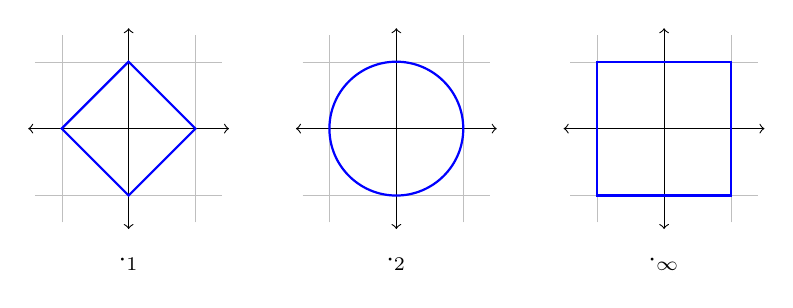
\begin{tikzpicture}[scale=0.85]
	% l^1
	\begin{scope}[xshift=0cm]
		\draw[ultra thin, color=lightgray] (-1.4,-1.4) grid (1.4,1.4);
		\draw[<->] (-1.5,0) -- (1.5,0);
		\draw[<->] (0,-1.5) -- (0,1.5);
		\draw[thick, color=blue] (1,0) -- (0,1) -- (-1,0) -- (0,-1) -- cycle;
		\node at (0,-2) {$\norm{\cdot}_1$};
	\end{scope}
	% l^2
	\begin{scope}[xshift=4cm]
		\draw[ultra thin, color=lightgray] (-1.4,-1.4) grid (1.4,1.4);
		\draw[<->] (-1.5,0) -- (1.5,0);
		\draw[<->] (0,-1.5) -- (0,1.5);
		\draw[thick, color=blue] (0,0) circle (1);
		\node at (0,-2) {$\norm{\cdot}_2$};
	\end{scope}
	% l^infty
	\begin{scope}[xshift=8cm]
		\draw[ultra thin, color=lightgray] (-1.4,-1.4) grid (1.4,1.4);
		\draw[<->] (-1.5,0) -- (1.5,0);
		\draw[<->] (0,-1.5) -- (0,1.5);
		\draw[thick, color=blue] (-1,-1) rectangle (1,1);
		\node at (0,-2) {$\norm{\cdot}_\infty$};
	\end{scope}
\end{tikzpicture}
\end{center}

As $p$ increases from $1$ to $\infty$ the unit ball swells continuously from the diamond out to the square, always staying convex and always containing the same four points $(\pm 1, 0)$, $(0, \pm 1)$. (Convexity of the ball is exactly the triangle inequality: if $\norm{v}, \norm{w} \leq 1$ and $t \in [0,1]$ then $\norm{tv + (1-t)w} \leq t + (1-t) = 1$. This is why $\norm{\cdot}_p$ is \emph{not} a norm for $p < 1$ -- the `ball' becomes a four-pointed star, and it is not convex.)

\begin{center}
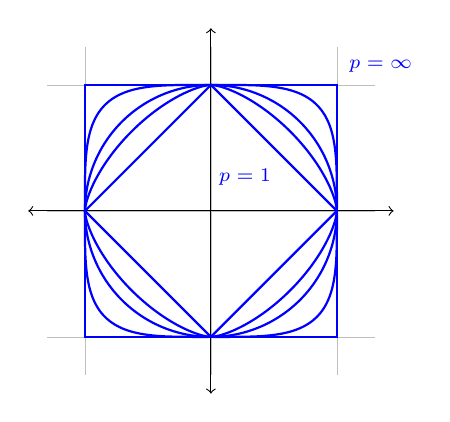
\begin{tikzpicture}[scale=1.6]
	\draw[ultra thin, color=lightgray] (-1.3,-1.3) grid (1.3,1.3);
	\draw[<->] (-1.45,0) -- (1.45,0);
	\draw[<->] (0,-1.45) -- (0,1.45);
	% p = 1 diamond
	\draw[thick, color=blue] (1,0) -- (0,1) -- (-1,0) -- (0,-1) -- cycle;
	% p = infinity square
	\draw[thick, color=blue] (-1,-1) rectangle (1,1);
	% general p curves
	\foreach \p in {1.5, 2, 4} {
		\foreach \sx in {1,-1} {
			\foreach \sy in {1,-1} {
				\draw[thick, color=blue, xscale=\sx, yscale=\sy]
					plot[domain=0.02:89.98, samples=70, smooth]
					({(cos(\x))^(2/\p)}, {(sin(\x))^(2/\p)});
			}
		}
	}
	\node[color=blue] at (0.27,0.27) {\scriptsize $p=1$};
	\node[color=blue, anchor=south west] at (1.02,1.02) {\scriptsize $p=\infty$};
\end{tikzpicture}
\end{center}

The curves drawn are $p = 1, \frac32, 2, 4, \infty$, and they nest outwards as $p$ increases.

Before we can prove Minkowski's inequality we need Hölder's, which is one of the workhorses of the subject. We say that $p, q \in [1, \infty]$ are \vocab{conjugate exponents} if
$$\frac{1}{p} + \frac{1}{q} = 1,$$
with the convention $1/\infty = 0$, so that $1$ and $\infty$ are conjugate to each other and $2$ is conjugate to itself.

\begin{lemma}[Young's Inequality]
	Let $p, q \in (1, \infty)$ be conjugate. Then for all $a, b \geq 0$,
	$$ab \leq \frac{a^p}{p} + \frac{b^q}{q}.$$
\end{lemma}

\begin{proof}
	If $a$ or $b$ is zero this is clear, so assume both are positive. The logarithm is concave, so
	$$\log\left( \frac{a^p}{p} + \frac{b^q}{q} \right) \geq \frac{1}{p} \log(a^p) + \frac{1}{q} \log(b^q) = \log a + \log b = \log(ab),$$
	and we exponentiate.
\end{proof}

\begin{proposition}[Hölder's Inequality]
	Let $p, q \in [1, \infty]$ be conjugate exponents. Then for $x, y \in \F^n$,
	$$\sum_{i=1}^n |x_i y_i| \leq \norm{x}_p \norm{y}_q.$$
\end{proposition}

\begin{proof}
	The cases $p = 1, q = \infty$ (and vice versa) are immediate, since $\sum |x_iy_i| \leq (\max_i |y_i|) \sum_i |x_i|$. So suppose $1 < p < \infty$. If either $x$ or $y$ is zero there is nothing to prove; otherwise, by homogeneity we may rescale and assume $\norm{x}_p = \norm{y}_q = 1$. Then Young's inequality gives
	$$\sum_{i=1}^n |x_i y_i| \leq \sum_{i=1}^n \left( \frac{|x_i|^p}{p} + \frac{|y_i|^q}{q} \right) = \frac{1}{p} + \frac{1}{q} = 1 = \norm{x}_p \norm{y}_q,$$
	as required.
\end{proof}

\begin{proposition}[Minkowski's Inequality]
	Let $1 \leq p \leq \infty$. Then for $x, y \in \F^n$,
	$$\norm{x + y}_p \leq \norm{x}_p + \norm{y}_p.$$
\end{proposition}

\begin{proof}
	Again $p = 1, \infty$ are clear, so take $1 < p < \infty$ and let $q$ be conjugate to $p$. We may assume $\norm{x+y}_p \neq 0$. Then
	\begin{align*}
		\norm{x+y}_p^p &= \sum_{i=1}^n |x_i + y_i| \cdot |x_i + y_i|^{p-1} \\
		&\leq \sum_{i=1}^n |x_i| \cdot |x_i + y_i|^{p-1} + \sum_{i=1}^n |y_i| \cdot |x_i + y_i|^{p-1} \\
		&\leq \left( \norm{x}_p + \norm{y}_p \right) \left( \sum_{i=1}^n |x_i + y_i|^{(p-1)q} \right)^{1/q},
	\end{align*}
	using Hölder on each sum. Since $(p-1)q = p$, the last bracket is $\norm{x+y}_p^{p/q}$. Dividing through by $\norm{x+y}_p^{p/q}$ and noting $p - p/q = 1$ gives the result.
\end{proof}

Exactly the same arguments work for infinite sums and for integrals, and we will use them in those settings without further comment.

\begin{example}[Sequence spaces]
	For $1 \leq p < \infty$ let
	$$\ell^p = \left\{ x = (x_1, x_2, \dots) : x_i \in \F, \ \sum_{i=1}^\infty |x_i|^p < \infty \right\}, \qquad \norm{x}_p = \left( \sum_{i=1}^\infty |x_i|^p \right)^{1/p},$$
	and let
	$$\ell^\infty = \left\{ x : \sup_i |x_i| < \infty \right\}, \qquad \norm{x}_\infty = \sup_i |x_i|.$$
	Minkowski's inequality (applied to partial sums and passing to the limit) shows both that $\ell^p$ is a vector space and that $\norm{\cdot}_p$ is a norm on it.

	Inside $\ell^\infty$ sit two further spaces which will be useful for producing counterexamples:
	$$c_0 = \{ x : x_i \to 0 \}, \qquad c_{00} = \{ x : x_i = 0 \text{ for all but finitely many } i \}.$$
	We give both the $\norm{\cdot}_\infty$ norm. Note $c_{00} \subseteq c_0 \subseteq \ell^\infty$, and in fact $c_{00}$ is dense in $c_0$ but not in $\ell^\infty$.
\end{example}

\begin{example}[Spaces of continuous functions]
	Let $K$ be a compact topological space (usually for us a closed bounded subset of $\R^n$, or a compact metric space). Write
	$$C(K) = \{ f : K \to \F \ \text{continuous} \}, \qquad \norm{f}_\infty = \sup_{x \in K} |f(x)|.$$
	The supremum is finite because a continuous function on a compact space is bounded, and it is attained. This is called the \vocab{uniform} or \vocab{supremum norm}, and convergence in it is exactly uniform convergence, as studied in IB Analysis and Topology.

	More generally, for any set $S$ we may take $B(S)$, the space of all bounded functions $S \to \F$, with the same norm.
\end{example}

\begin{example}[$L^p$ spaces]
	For $1 \leq p < \infty$ define on $C[0,1]$ the norm
	$$\norm{f}_{L^p} = \left( \int_0^1 |f(x)|^p \dd x \right)^{1/p}.$$
	The integral version of Minkowski's inequality gives the triangle inequality, and $\norm{f}_{L^p} = 0$ forces $f = 0$ because a non-zero continuous function is bounded away from zero on some interval. So this is a norm.

	It is, however, a rather badly behaved one: as we will see, $(C[0,1], \norm{\cdot}_{L^p})$ is not complete. One writes $L^p[0,1]$ for its completion. In IID Probability and Measure you will see that this completion can be described concretely as the space of $p$-integrable measurable functions modulo equality almost everywhere, but we will not need that here -- for us $L^p$ is simply `the completion of the continuous functions'.
\end{example}

\begin{example}[Subspaces and products]
	Any linear subspace $W$ of a normed space $V$ is a normed space with the restricted norm. If $V, W$ are normed spaces then $V \oplus W$ becomes one via, say, $\norm{(v,w)} = \norm{v}_V + \norm{w}_W$, and the topology this induces is the product topology.
\end{example}

There is one more construction we will want, and it is a little less obvious.

\begin{proposition}[Quotient norm]
	Let $V$ be a normed space and $W \subseteq V$ a \emph{closed} subspace. Then
	$$\norm{v + W}_{V/W} = \inf_{w \in W} \norm{v + w} = \dist(v, W)$$
	defines a norm on the quotient vector space $V/W$.
\end{proposition}

\begin{proof}
	Homogeneity and the triangle inequality are straightforward: for the latter, given $\varepsilon > 0$ pick $w_1, w_2 \in W$ with $\norm{v_i + w_i} \leq \norm{v_i + W} + \varepsilon$, and then $\norm{(v_1 + v_2) + (w_1 + w_2)} \leq \norm{v_1 + W} + \norm{v_2 + W} + 2\varepsilon$.

	For positivity, suppose $\norm{v + W} = 0$. Then there are $w_n \in W$ with $\norm{v + w_n} \to 0$, so $-w_n \to v$, and since $W$ is closed we get $v \in W$, i.e.\ $v + W = 0$ in $V/W$. This is exactly where closedness is needed: without it we would only get a seminorm.
\end{proof}

\subsection{Completeness and Banach Spaces}

The single most important extra hypothesis in this course is completeness. Recall from IB Analysis and Topology that a metric space is complete if every Cauchy sequence converges.

\begin{definition}[Banach space]
	A normed space which is complete in the induced metric is called a \vocab{Banach space}.
\end{definition}

Completeness is what lets us construct things: we build a candidate solution as a limit of approximations, and completeness guarantees that the limit exists. Almost every theorem in this course that produces something out of nothing uses completeness somewhere.

Let's check our examples.

\begin{proposition}
	For any set $S$, the space $B(S)$ of bounded functions $S \to \F$ with the supremum norm is a Banach space. Consequently so is $C(K)$ for $K$ compact, and so is $\ell^\infty$.
\end{proposition}

\begin{proof}
	Let $(f_n)$ be Cauchy in $B(S)$. For each fixed $x \in S$ we have $|f_n(x) - f_m(x)| \leq \norm{f_n - f_m}_\infty$, so $(f_n(x))$ is Cauchy in $\F$ and therefore converges; call the limit $f(x)$.

	Given $\varepsilon > 0$, choose $N$ with $\norm{f_n - f_m}_\infty < \varepsilon$ for $n, m \geq N$. Fixing $n \geq N$ and $x \in S$ and letting $m \to \infty$ in $|f_n(x) - f_m(x)| < \varepsilon$ gives $|f_n(x) - f(x)| \leq \varepsilon$. As $x$ was arbitrary, $\norm{f_n - f}_\infty \leq \varepsilon$ for all $n \geq N$. In particular $f$ is bounded (being within $\varepsilon$ of the bounded function $f_N$) and $f_n \to f$ in $B(S)$.

	For $C(K)$: it is a subspace of $B(K)$, and a closed one, because a uniform limit of continuous functions is continuous. A closed subspace of a complete space is complete. Finally $\ell^\infty = B(\N)$.
\end{proof}

\begin{proposition}
	For $1 \leq p < \infty$, $\ell^p$ is a Banach space. So are $c_0$ and $c$ (the space of convergent sequences), with the supremum norm.
\end{proposition}

\begin{proof}
	Let $(x^{(n)})$ be Cauchy in $\ell^p$. For each coordinate $i$ we have $|x_i^{(n)} - x_i^{(m)}| \leq \norm{x^{(n)} - x^{(m)}}_p$, so each coordinate sequence is Cauchy in $\F$; let $x_i = \lim_n x_i^{(n)}$ and $x = (x_1, x_2, \dots)$.

	Let $\varepsilon > 0$ and pick $N$ with $\norm{x^{(n)} - x^{(m)}}_p < \varepsilon$ for $n, m \geq N$. For any fixed $K \in \N$ and $n, m \geq N$,
	$$\sum_{i=1}^K |x_i^{(n)} - x_i^{(m)}|^p < \varepsilon^p.$$
	Letting $m \to \infty$ (a finite sum, so no issue) gives $\sum_{i=1}^K |x_i^{(n)} - x_i|^p \leq \varepsilon^p$, and now letting $K \to \infty$ gives $\norm{x^{(n)} - x}_p \leq \varepsilon$. In particular $x^{(n)} - x \in \ell^p$, so $x = x^{(n)} - (x^{(n)} - x) \in \ell^p$, and $x^{(n)} \to x$.

	For $c_0$ and $c$: both are subspaces of $\ell^\infty$, and both are closed, since a uniform limit of sequences tending to $0$ tends to $0$, and a uniform limit of convergent sequences is convergent (this is the same interchange-of-limits argument as for continuity).
\end{proof}

\begin{example}[An incomplete normed space]
	The space $c_{00}$ of finitely supported sequences with $\norm{\cdot}_\infty$ is \emph{not} complete. Indeed take
	$$x^{(n)} = (1, \tfrac{1}{2}, \tfrac{1}{3}, \dots, \tfrac{1}{n}, 0, 0, \dots).$$
	Then $\norm{x^{(n)} - x^{(m)}}_\infty = 1/(\min(n,m)+1) \to 0$, so the sequence is Cauchy, but the only possible limit is $(1, \frac12, \frac13, \dots)$, which is not in $c_{00}$. The point is that $c_{00}$ is a dense but proper subspace of $c_0$.
\end{example}

\begin{example}[{$C[0,1]$ with the $L^1$ norm is incomplete}]
	Consider the continuous functions
	$$f_n(x) = \begin{cases} 0 & 0 \leq x \leq \tfrac12, \\ n(x - \tfrac12) & \tfrac12 \leq x \leq \tfrac12 + \tfrac1n, \\ 1 & \tfrac12 + \tfrac1n \leq x \leq 1.\end{cases}$$
	\begin{center}
	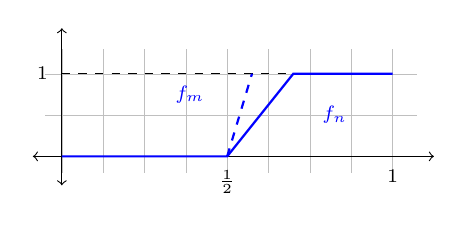
\begin{tikzpicture}[scale=1.05]
		\draw[ultra thin, color=lightgray, step=0.5] (-0.2,-0.2) grid (4.3,1.3);
		\draw[<->] (-0.35,0) -- (4.5,0);
		\draw[<->] (0,-0.35) -- (0,1.55);
		\draw[dashed] (0,1) -- (4,1);
		\draw[thick, color=blue] (0,0) -- (2,0) -- (2.8,1) -- (4,1);
		\draw[thick, color=blue, dashed] (2,0) -- (2.3,1);
		\node[color=blue] at (3.3,0.5) {\scriptsize $f_n$};
		\node[color=blue] at (1.55,0.75) {\scriptsize $f_m$};
		\node[below] at (2,-0.05) {\scriptsize $\frac12$};
		\node[below] at (4,-0.05) {\scriptsize $1$};
		\node[left] at (-0.05,1) {\scriptsize $1$};
	\end{tikzpicture}
	\end{center}
	For $m > n$ we have $\norm{f_n - f_m}_{L^1} \leq 1/n \to 0$, so $(f_n)$ is Cauchy. If $f_n \to f$ in $L^1$ with $f$ continuous, then on $[0, \frac12]$ we would need $\int_0^{1/2}|f| = 0$, so $f \equiv 0$ there, and on $[\frac12 + \delta, 1]$ we would need $f \equiv 1$ for every $\delta > 0$. No continuous function does both. So $(C[0,1], \norm{\cdot}_{L^1})$ is not complete.
\end{example}

\subsection{Series in Normed Spaces}

In a normed space we can add up infinitely many vectors, provided the partial sums converge. It turns out that the interaction between two natural notions of convergence for series characterises completeness exactly, which is a pleasant surprise and often the most convenient way to check that a space is Banach.

\begin{definition}[Convergence of series]
	Let $V$ be a normed space and $(v_n)$ a sequence in $V$. We say $\sum_{n=1}^\infty v_n$ \vocab{converges} to $v \in V$ if the partial sums $s_N = \sum_{n=1}^N v_n$ satisfy $s_N \to v$. We say the series is \vocab{absolutely convergent} if $\sum_{n=1}^\infty \norm{v_n} < \infty$.
\end{definition}

In $\R$, absolute convergence implies convergence, and the proof uses the completeness of $\R$ in an essential way. The same is true in any Banach space, and conversely.

\begin{theorem}[Series criterion for completeness]
	A normed space $V$ is a Banach space if and only if every absolutely convergent series in $V$ converges.
\end{theorem}

\begin{proof}
	($\Rightarrow$) Suppose $V$ is complete and $\sum \norm{v_n} < \infty$. For $M > N$,
	$$\norm{s_M - s_N} = \left\| \sum_{n=N+1}^M v_n \right\| \leq \sum_{n=N+1}^M \norm{v_n} \leq \sum_{n > N} \norm{v_n},$$
	which tends to $0$ as $N \to \infty$ since the tail of a convergent series of reals tends to zero. So $(s_N)$ is Cauchy, hence convergent.

	($\Leftarrow$) Suppose every absolutely convergent series converges, and let $(x_n)$ be a Cauchy sequence in $V$. Choose a subsequence as follows: pick $n_1 < n_2 < \cdots$ such that
	$$\norm{x_n - x_m} < 2^{-k} \quad \text{for all } n, m \geq n_k.$$
	Set $v_1 = x_{n_1}$ and $v_k = x_{n_k} - x_{n_{k-1}}$ for $k \geq 2$, so that $\sum_{k=1}^K v_k = x_{n_K}$. Then $\norm{v_k} < 2^{-(k-1)}$ for $k \geq 2$, so $\sum \norm{v_k} < \infty$ and by hypothesis $\sum v_k$ converges, i.e.\ $x_{n_K} \to x$ for some $x \in V$.

	Finally, a Cauchy sequence with a convergent subsequence converges: given $\varepsilon > 0$, take $N$ with $\norm{x_n - x_m} < \varepsilon/2$ for $n,m \geq N$ and $K$ with $n_K \geq N$ and $\norm{x_{n_K} - x} < \varepsilon/2$; then $\norm{x_n - x} < \varepsilon$ for $n \geq N$.
\end{proof}

\begin{remark}
	The subsequence trick in the second half is worth remembering in its own right: \emph{every Cauchy sequence has a rapidly Cauchy subsequence}, one where the successive differences are summable. It reappears in measure theory and in the proof of the open mapping theorem.
\end{remark}

Here is a typical application, which also gives us a supply of Banach spaces we did not have before.

\begin{proposition}
	Let $V$ be a Banach space and $W \subseteq V$ a closed subspace. Then $W$ and $V/W$ are both Banach spaces.
\end{proposition}

\begin{proof}
	That $W$ is complete is standard (a closed subset of a complete metric space is complete). For $V/W$ we use the series criterion. Let $\sum_n \norm{v_n + W} < \infty$. For each $n$ pick $w_n \in W$ with
	$$\norm{v_n + w_n} \leq \norm{v_n + W} + 2^{-n}.$$
	Then $\sum_n \norm{v_n + w_n} < \infty$, so by completeness of $V$ the series $\sum_n (v_n + w_n)$ converges to some $v \in V$. Since the quotient map $q : V \to V/W$ satisfies $\norm{q(u)} \leq \norm{u}$, it is continuous, and hence
	$$\sum_{n=1}^N (v_n + W) = q\left( \sum_{n=1}^N (v_n + w_n) \right) \longrightarrow q(v)$$
	as $N \to \infty$. So the series converges in $V/W$.
\end{proof}

\subsection{Completions}

We remarked above that $L^p[0,1]$ is `the completion' of $C[0,1]$. Let us make sure that makes sense.

\begin{theorem}[Completion]
	Let $V$ be a normed space. Then there is a Banach space $\bar{V}$ and a linear isometry $\iota : V \to \bar{V}$ with $\iota(V)$ dense in $\bar{V}$. Moreover $\bar{V}$ is unique up to isometric isomorphism.
\end{theorem}

\begin{proof}[Proof sketch]
	One route is the standard metric space completion from IB Analysis and Topology: take Cauchy sequences in $V$ modulo the equivalence $(x_n) \sim (y_n)$ iff $\norm{x_n - y_n} \to 0$. The vector space operations and the norm $\norm{[(x_n)]} = \lim_n \norm{x_n}$ descend to this set, and one checks the axioms.

	A slicker route, available once we have the Hahn--Banach theorem, is to embed $V$ isometrically into the Banach space $\ell^\infty(\bar{B}_{V^*})$ and take the closure of the image; we will see this idea again when we discuss the double dual.

	Uniqueness: if $\iota_1 : V \to X_1$ and $\iota_2 : V \to X_2$ are two such, then $\iota_2 \circ \iota_1^{-1}$ is an isometry defined on the dense subspace $\iota_1(V)$ of $X_1$, and a uniformly continuous map into a complete space extends uniquely to the closure.
\end{proof}

We will use completions sparingly, but it is comforting to know they exist: it means that when we prove a theorem about Banach spaces, we have not narrowed our attention as much as it might appear.

\subsection{Finite-Dimensional Spaces}

Finite-dimensional normed spaces are, from the point of view of this course, thoroughly boring -- and it is worth understanding exactly \emph{how} boring, because that tells us what to expect (or rather, what not to expect) in infinite dimensions. The headline is that a finite-dimensional space has essentially only one norm.

\begin{definition}[Equivalent norms]
	Two norms $\norm{\cdot}_a$ and $\norm{\cdot}_b$ on a vector space $V$ are \vocab{equivalent} if there is a constant $C \geq 1$ with
	$$C^{-1} \norm{v}_b \leq \norm{v}_a \leq C \norm{v}_b \qquad \text{for all } v \in V.$$
\end{definition}

This is an equivalence relation, and equivalent norms have the same open sets, the same convergent sequences, the same Cauchy sequences and the same compact sets -- essentially, everything we care about is unaffected.

\begin{theorem}[Equivalence of norms in finite dimensions]
	Let $V$ be a finite-dimensional vector space over $\F$. Then any two norms on $V$ are equivalent.
\end{theorem}

\begin{proof}
	Fix a basis $e_1, \dots, e_n$ of $V$ and let $\norm{\cdot}_1$ denote the associated $\ell^1$ norm, $\norm{\sum_i \lambda_i e_i}_1 = \sum_i |\lambda_i|$. Since equivalence is transitive, it suffices to show that an arbitrary norm $\norm{\cdot}$ is equivalent to $\norm{\cdot}_1$.

	One direction is easy: writing $v = \sum_i \lambda_i e_i$,
	$$\norm{v} \leq \sum_{i=1}^n |\lambda_i| \norm{e_i} \leq C \norm{v}_1, \qquad C := \max_i \norm{e_i},$$
	which is finite as it is a maximum over a finite set.

	For the other direction, let $S = \{v \in V : \norm{v}_1 = 1\}$. The inequality just proved shows that $\norm{\cdot} : (V, \norm{\cdot}_1) \to \R$ is continuous, since
	$$\big| \norm{v} - \norm{w} \big| \leq \norm{v - w} \leq C\norm{v-w}_1.$$
	Also $S$ is compact in $(V, \norm{\cdot}_1)$: identifying $V$ with $\F^n$ via the basis, $S$ is the unit sphere of $\ell_1^n$, which is closed and bounded, hence compact by Bolzano--Weierstrass (applied coordinate by coordinate, extracting subsequences $n$ times).

	Therefore $\norm{\cdot}$ attains its infimum on $S$, say at $v_*$. Since $v_* \in S$ we have $v_* \neq 0$, so $c := \norm{v_*} > 0$, and $\norm{v} \geq c$ for all $v \in S$. For general $v \neq 0$, applying this to $v / \norm{v}_1 \in S$ gives $\norm{v} \geq c \norm{v}_1$. Taking $\max(C, c^{-1})$ finishes the proof.
\end{proof}

Several pleasant consequences follow immediately.

\begin{corollary}
	Let $V$ be a finite-dimensional normed space. Then:
	\begin{enumerate}[label=(\roman*)]
		\item $V$ is a Banach space;
		\item the closed unit ball $\bar{B}_V$ is compact;
		\item any linear map from $V$ to a normed space $W$ is continuous;
		\item any finite-dimensional subspace of a normed space is closed.
	\end{enumerate}
\end{corollary}

\begin{proof}
	By the theorem we may compute in $\ell_1^n$, which is complete and in which closed bounded sets are compact; this gives (i) and (ii). For (iii), if $T : V \to W$ is linear then $\norm{v}' := \norm{v}_V + \norm{Tv}_W$ is a norm on $V$, hence equivalent to $\norm{\cdot}_V$, so $\norm{Tv}_W \leq \norm{v}' \leq C \norm{v}_V$; and a linear map satisfying such a bound is continuous, as we check in the next section. For (iv), a complete subspace of a metric space is closed.
\end{proof}

Part (ii) is the interesting one, because it turns out to \emph{characterise} finite dimensionality. The key is the following geometric lemma, which says that from any proper closed subspace we can always step almost perpendicularly away.

\begin{lemma}[Riesz's Lemma]
	Let $X$ be a normed space and $Y \subsetneq X$ a closed proper subspace. Then for every $\theta \in (0,1)$ there exists $x \in X$ with $\norm{x} = 1$ and
	$$\dist(x, Y) = \inf_{y \in Y} \norm{x - y} \geq \theta.$$
\end{lemma}

\begin{proof}
	Pick any $z \in X \setminus Y$. Since $Y$ is closed, $d := \dist(z, Y) > 0$. As $\theta < 1$ we have $d < d/\theta$, so by definition of the infimum there is some $y_0 \in Y$ with
	$$d \leq \norm{z - y_0} \leq \frac{d}{\theta}.$$
	Set
	$$x = \frac{z - y_0}{\norm{z - y_0}},$$
	so $\norm{x} = 1$. For any $y \in Y$,
	$$\norm{x - y} = \frac{1}{\norm{z - y_0}} \norm{ z - y_0 - \norm{z - y_0} y } = \frac{\norm{z - y'}}{\norm{z-y_0}}$$
	where $y' = y_0 + \norm{z - y_0}y \in Y$. Hence $\norm{z - y'} \geq d$, and so
	$$\norm{x - y} \geq \frac{d}{\norm{z - y_0}} \geq \frac{d}{d/\theta} = \theta,$$
	as required.
\end{proof}

Geometrically, we take a point $z$ off the subspace, find a point $y_0 \in Y$ that very nearly realises the distance from $z$ to $Y$, and then rescale the difference to have length one. The resulting unit vector sticks out of $Y$ by almost its full length.

\begin{center}
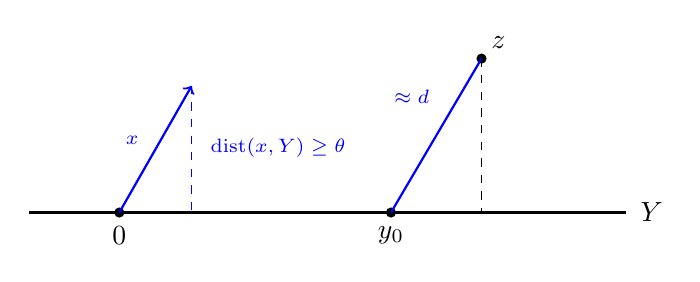
\begin{tikzpicture}[scale=1.15]
	% subspace Y as a horizontal line
	\draw[thick] (-3.4,0) -- (3.2,0);
	\node[right] at (3.25,0) {$Y$};
	% point z
	\fill (1.6,1.7) circle (1.6pt);
	\node[above right] at (1.6,1.7) {$z$};
	% nearest-ish point y0
	\fill (0.6,0) circle (1.6pt);
	\node[below] at (0.6,-0.05) {$y_0$};
	% segment z - y0
	\draw[thick, color=blue] (0.6,0) -- (1.6,1.7);
	\node[color=blue, left] at (1.13,1.28) {\scriptsize $\approx d$};
	% dashed foot of perpendicular from z
	\draw[dashed] (1.6,1.7) -- (1.6,0);
	% unit vector x drawn from origin
	\fill (-2.4,0) circle (1.6pt);
	\node[below] at (-2.4,-0.05) {$0$};
	\draw[->, thick, color=blue] (-2.4,0) -- (-1.6,1.4);
	\node[color=blue, left] at (-2.08,0.8) {\scriptsize $x$};
	% dashed drop showing the distance to Y
	\draw[dashed, color=blue] (-1.6,1.4) -- (-1.6,0);
	\node[color=blue, right] at (-1.5,0.72) {\scriptsize $\dist(x,Y) \geq \theta$};
\end{tikzpicture}
\end{center}

\begin{theorem}[Riesz]
	Let $X$ be a normed space. Then the closed unit ball $\bar{B}_X$ is compact if and only if $X$ is finite-dimensional.
\end{theorem}

\begin{proof}
	We have already seen ($\Leftarrow$). For ($\Rightarrow$), suppose $X$ is infinite-dimensional. We build a sequence $(x_n)$ of unit vectors with $\norm{x_n - x_m} \geq \frac12$ for $n \neq m$; such a sequence has no convergent subsequence, so $\bar{B}_X$ is not (sequentially, hence not) compact.

	Take any unit vector $x_1$. Having chosen $x_1, \dots, x_n$, let $Y_n = \spn\{x_1, \dots, x_n\}$. This is finite-dimensional, hence closed, and it is proper because $X$ is infinite-dimensional. By Riesz's lemma with $\theta = \frac12$ there is a unit vector $x_{n+1}$ with $\dist(x_{n+1}, Y_n) \geq \frac12$, and in particular $\norm{x_{n+1} - x_j} \geq \frac12$ for all $j \leq n$.
\end{proof}

\begin{example}
	In $\ell^p$ (any $1 \leq p \leq \infty$) the standard unit vectors $e_n = (0, \dots, 0, 1, 0, \dots)$ satisfy $\norm{e_n}_p = 1$ and $\norm{e_n - e_m}_p = 2^{1/p}$ for $n \neq m$ (interpreted as $1$ when $p = \infty$). So we can see the failure of compactness with our bare hands, without invoking Riesz's lemma.
\end{example}

This is the first genuinely infinite-dimensional phenomenon we have met, and it is a serious one. In $\R^n$, `closed and bounded' is the same as `compact', and compactness is what makes extremal problems solvable -- continuous functions attain their bounds, sequences have convergent subsequences. In infinite dimensions all of that is gone. A great deal of this course consists of finding substitutes.

\section{Bounded Linear Operators}

Having set up our objects, we now turn to the maps between them. In linear algebra the maps of interest were the linear ones; here we want them to be linear \emph{and} continuous. The pleasant surprise is that for linear maps, continuity has a very concrete reformulation.

\subsection{Boundedness and the Operator Norm}

\begin{definition}[Bounded linear map]
	Let $X, Y$ be normed spaces. A linear map $T : X \to Y$ is \vocab{bounded} if there is a constant $C \geq 0$ with
	$$\norm{Tx}_Y \leq C \norm{x}_X \qquad \text{for all } x \in X.$$
	We write $\Bop(X,Y)$ for the set of bounded linear maps $X \to Y$, and $\Bop(X) = \Bop(X,X)$.
\end{definition}

Note that `bounded' here does \emph{not} mean `has bounded image' -- no non-zero linear map has bounded image. It means `bounded on the unit ball', which by linearity is the same as the displayed condition.

\begin{proposition}
	Let $T : X \to Y$ be linear. The following are equivalent:
	\begin{enumerate}[label=(\roman*)]
		\item $T$ is continuous;
		\item $T$ is continuous at $0$;
		\item $T$ is bounded;
		\item $T$ is Lipschitz.
	\end{enumerate}
\end{proposition}

\begin{proof}
	(i) $\Rightarrow$ (ii) is trivial and (iv) $\Rightarrow$ (i) is standard.

	(ii) $\Rightarrow$ (iii). By continuity at $0$ there is $\delta > 0$ such that $\norm{x} \leq \delta$ implies $\norm{Tx} \leq 1$. For general $x \neq 0$, apply this to $\delta x / \norm{x}$ to get $\norm{Tx} \leq \delta^{-1} \norm{x}$.

	(iii) $\Rightarrow$ (iv). If $\norm{Tx} \leq C\norm{x}$ then $\norm{Tx - Tx'} = \norm{T(x - x')} \leq C \norm{x - x'}$.
\end{proof}

So continuity is a purely quantitative matter, and we may as well keep track of the best constant.

\begin{definition}[Operator norm]
	For $T \in \Bop(X,Y)$, the \vocab{operator norm} of $T$ is
	$$\norm{T} = \sup_{x \neq 0} \frac{\norm{Tx}_Y}{\norm{x}_X} = \sup_{\norm{x} \leq 1} \norm{Tx}_Y = \sup_{\norm{x} = 1} \norm{Tx}_Y.$$
\end{definition}

The three expressions agree by homogeneity (the last requires $X \neq \{0\}$). By construction $\norm{Tx} \leq \norm{T}\norm{x}$, and $\norm{T}$ is the least constant with this property.

\begin{proposition}
	$\Bop(X,Y)$ is a vector space and $\norm{\cdot}$ is a norm on it. Moreover if $T \in \Bop(X,Y)$ and $S \in \Bop(Y,Z)$ then $ST \in \Bop(X,Z)$ with
	$$\norm{ST} \leq \norm{S} \norm{T}.$$
\end{proposition}

\begin{proof}
	If $\norm{T} = 0$ then $Tx = 0$ for all $x$, so $T = 0$. Homogeneity is clear, and for the triangle inequality,
	$$\norm{(S+T)x} \leq \norm{Sx} + \norm{Tx} \leq (\norm{S} + \norm{T})\norm{x},$$
	so $\norm{S+T} \leq \norm{S} + \norm{T}$. Finally $\norm{STx} \leq \norm{S}\norm{Tx} \leq \norm{S}\norm{T}\norm{x}$.
\end{proof}

The last inequality says that $\Bop(X)$ is a \vocab{normed algebra}: it is an algebra under composition, and the norm is submultiplicative. If $X$ is a Banach space it is a \vocab{Banach algebra}, by the next result.

\begin{theorem}
	If $Y$ is a Banach space then $\Bop(X,Y)$ is a Banach space, for any normed space $X$.
\end{theorem}

\begin{proof}
	Let $(T_n)$ be Cauchy in $\Bop(X,Y)$. For each $x \in X$,
	$$\norm{T_n x - T_m x} \leq \norm{T_n - T_m}\norm{x},$$
	so $(T_n x)$ is Cauchy in $Y$, hence converges; define $Tx = \lim_n T_n x$. The map $T$ is linear, being a pointwise limit of linear maps.

	Cauchy sequences are bounded, say $\norm{T_n} \leq M$; then $\norm{Tx} = \lim_n \norm{T_n x} \leq M \norm{x}$, so $T$ is bounded.

	Finally, given $\varepsilon > 0$ take $N$ with $\norm{T_n - T_m} < \varepsilon$ for $n, m \geq N$. For $\norm{x} \leq 1$ and $n \geq N$,
	$$\norm{T_n x - Tx} = \lim_{m \to \infty} \norm{T_n x - T_m x} \leq \varepsilon,$$
	and taking the supremum over such $x$ gives $\norm{T_n - T} \leq \varepsilon$. So $T_n \to T$ in operator norm.
\end{proof}

Note carefully that completeness of $X$ played no role. This is a recurring theme: it is the \emph{target} that needs to be complete.

\begin{example}
	\begin{enumerate}[label=(\roman*)]
		\item Let $X = \ell^p$ and let $\lambda = (\lambda_n)$ be a bounded sequence. The \vocab{diagonal operator} $M_\lambda x = (\lambda_n x_n)$ is bounded with $\norm{M_\lambda} = \norm{\lambda}_\infty$. Indeed $\norm{M_\lambda x}_p \leq \norm{\lambda}_\infty \norm{x}_p$, and testing on $e_n$ gives $\norm{M_\lambda} \geq |\lambda_n|$ for each $n$.
		\item The \vocab{right shift} $R : \ell^p \to \ell^p$, $R(x_1, x_2, \dots) = (0, x_1, x_2, \dots)$, is an isometry, so $\norm{R} = 1$. It is injective but not surjective. The \vocab{left shift} $L(x_1, x_2, \dots) = (x_2, x_3, \dots)$ has $\norm{L} = 1$, and is surjective but not injective. In finite dimensions no linear map can behave like either of these; this is the rank-nullity theorem failing to have an infinite-dimensional analogue.
		\item Let $k \in C([0,1]^2)$ and define $T : C[0,1] \to C[0,1]$ by
		$$(Tf)(x) = \int_0^1 k(x,y) f(y) \dd y.$$
		This is the \vocab{integral operator} with kernel $k$. It is bounded, with $\norm{T} \leq \sup_{x} \int_0^1 |k(x,y)| \dd y \leq \norm{k}_\infty$. These operators will be our main source of examples of compact operators.
		\item Differentiation $\frac{\dd}{\dd x} : C^1[0,1] \to C[0,1]$ is \emph{unbounded} when $C^1[0,1]$ is given the sup norm: take $f_n(x) = \sin(n^2x)/n$, so $\norm{f_n}_\infty \leq 1/n \to 0$ but $\norm{f_n'}_\infty = n \to \infty$. Unboundedness of differentiation is the reason a great deal of analysis is hard.
	\end{enumerate}
\end{example}

\begin{proposition}
	Let $X$ be a normed space, $Y$ a Banach space and $Z \subseteq X$ a dense subspace. Then every $T \in \Bop(Z, Y)$ extends uniquely to $\wt{T} \in \Bop(X,Y)$, and $\norm{\wt T} = \norm{T}$.
\end{proposition}

\begin{proof}
	Given $x \in X$ pick $z_n \in Z$ with $z_n \to x$. Then $(z_n)$ is Cauchy, so $\norm{Tz_n - Tz_m} \leq \norm{T} \norm{z_n - z_m}$ shows $(Tz_n)$ is Cauchy in $Y$, and we set $\wt{T}x = \lim_n Tz_n$. This is independent of the choice of sequence (interleave two such sequences), and linearity passes to the limit. Also $\norm{\wt T x} = \lim \norm{Tz_n} \leq \norm{T}\lim\norm{z_n} = \norm{T}\norm{x}$, so $\norm{\wt T} \leq \norm{T}$; the reverse is clear as $\wt T$ extends $T$. Uniqueness holds because two continuous maps agreeing on a dense set agree everywhere.
\end{proof}

\subsection{Isomorphisms}

\begin{definition}[Isomorphism]
	A linear map $T : X \to Y$ between normed spaces is an \vocab{isomorphism} if it is a bijection and both $T$ and $T^{-1}$ are bounded. If in addition $\norm{Tx} = \norm{x}$ for all $x$, we call $T$ an \vocab{isometric isomorphism} and say $X$ and $Y$ are \vocab{isometrically isomorphic}, written $X \cong Y$.
\end{definition}

Being an isomorphism is equivalent to there existing $c, C > 0$ with $c\norm{x} \leq \norm{Tx} \leq C\norm{x}$ and $T$ surjective. The lower bound alone says $T$ is \vocab{bounded below}, which is equivalent to $T$ being injective with closed range.

\begin{proposition}
	Let $X$ be a Banach space and $T \in \Bop(X)$ with $\norm{T} < 1$. Then $I - T$ is invertible in $\Bop(X)$, with
	$$(I - T)^{-1} = \sum_{n=0}^\infty T^n,$$
	the series converging in operator norm. Moreover $\norm{(I-T)^{-1}} \leq (1 - \norm{T})^{-1}$.
\end{proposition}

\begin{proof}
	Since $\norm{T^n} \leq \norm{T}^n$ and $\norm{T} < 1$, the series $\sum_n T^n$ is absolutely convergent in $\Bop(X)$, which is a Banach space; so it converges, to $S$ say, and $\norm{S} \leq \sum_n \norm{T}^n = (1-\norm{T})^{-1}$. Writing $S_N = \sum_{n=0}^N T^n$ we have
	$$(I - T)S_N = S_N(I-T) = I - T^{N+1} \longrightarrow I,$$
	since $\norm{T^{N+1}} \to 0$. As multiplication in $\Bop(X)$ is continuous, letting $N \to \infty$ gives $(I-T)S = S(I-T) = I$.
\end{proof}

This is the \vocab{Neumann series}, and it is the workhorse of spectral theory. An immediate consequence is that the invertible elements of $\Bop(X)$ form an open set: if $T$ is invertible and $\norm{S - T} < \norm{T^{-1}}^{-1}$ then $S = T(I - T^{-1}(T-S))$ is invertible.

\subsection{Dual Spaces}

Among all bounded operators, those with target $\F$ deserve a special name.

\begin{definition}[Dual space]
	Let $X$ be a normed space. Its \vocab{dual space} is
	$$X^* = \Bop(X, \F),$$
	whose elements are called \vocab{bounded linear functionals} on $X$.
\end{definition}

Since $\F$ is complete, $X^*$ is \emph{always} a Banach space, whether or not $X$ is. This is a very useful piece of leverage: even for a horrible normed space $X$, the dual is a nice object.

In IB Linear Algebra we studied the dual $V'$ of a finite-dimensional space and found $\dim V' = \dim V$. In infinite dimensions the \emph{algebraic} dual (all linear functionals) is enormous and useless; it is the topological dual $X^*$ that carries information. It is not even obvious at this stage that $X^* \neq \{0\}$ for a general normed space $X$ -- that will be a consequence of the Hahn--Banach theorem.

Let's compute some duals.

\begin{proposition}
	For $1 < p < \infty$ with conjugate exponent $q$, we have $(\ell^p)^* \cong \ell^q$. Also $(\ell^1)^* \cong \ell^\infty$ and $(c_0)^* \cong \ell^1$.
\end{proposition}

\begin{proof}
	We do the case $1 \leq p < \infty$, the argument for $c_0$ being similar. Define $\Phi : \ell^q \to (\ell^p)^*$ by
	$$(\Phi y)(x) = \sum_{n=1}^\infty x_n y_n.$$
	By Hölder this converges with $|(\Phi y)(x)| \leq \norm{x}_p \norm{y}_q$, so $\Phi y \in (\ell^p)^*$ with $\norm{\Phi y} \leq \norm{y}_q$. It is clearly linear in $y$.

	\emph{$\Phi$ is isometric.} Suppose first $1 < p < \infty$. Given $y \in \ell^q$ non-zero, set $x_n = |y_n|^{q-1} \overline{\sgn(y_n)}$ where $\sgn(y) = y/|y|$ (and $x_n = 0$ if $y_n = 0$). Then $|x_n|^p = |y_n|^{(q-1)p} = |y_n|^q$, so $x \in \ell^p$ with $\norm{x}_p = \norm{y}_q^{q/p}$, while
	$$(\Phi y)(x) = \sum_n |y_n|^q = \norm{y}_q^q.$$
	Hence $\norm{\Phi y} \geq \norm{y}_q^{q - q/p} = \norm{y}_q$. For $p = 1, q = \infty$, test instead on $x = e_n$ to get $\norm{\Phi y} \geq |y_n|$ for each $n$.

	\emph{$\Phi$ is surjective.} Let $f \in (\ell^p)^*$ and put $y_n = f(e_n)$. For any $N$, applying $f$ to $x = \sum_{n \leq N} |y_n|^{q-1}\overline{\sgn(y_n)}e_n$ and using $|f(x)| \leq \norm{f}\norm{x}_p$ exactly as above gives
	$$\left(\sum_{n \leq N} |y_n|^q\right)^{1/q} \leq \norm{f}.$$
	Letting $N \to \infty$ shows $y \in \ell^q$ with $\norm{y}_q \leq \norm{f}$. Finally, $f$ and $\Phi y$ are bounded functionals agreeing on each $e_n$, hence on $c_{00}$, which is dense in $\ell^p$ for $p < \infty$; so $f = \Phi y$.
\end{proof}

\begin{remark}
	The density of $c_{00}$ is what fails for $p = \infty$, and indeed $(\ell^\infty)^* \neq \ell^1$: the dual of $\ell^\infty$ is strictly bigger, containing exotic objects called \emph{Banach limits} which one constructs with Hahn--Banach. So duality is not symmetric: we have $(\ell^1)^* = \ell^\infty$ but $(\ell^\infty)^* \supsetneq \ell^1$.
\end{remark}

\begin{example}
	If $X$ is finite-dimensional with basis $e_1, \dots, e_n$, then every linear functional is bounded, and $X^*$ is spanned by the dual basis $e_1^*, \dots, e_n^*$. In particular $(\ell_p^n)^* \cong \ell_q^n$ isometrically, by the same computation as above.
\end{example}

The dual of $C(K)$ is also computable, but the answer -- the space of regular Borel measures on $K$, by the Riesz--Markov theorem -- needs measure theory, so we will leave it aside. The one dual we will compute completely, and rather beautifully, is that of a Hilbert space.

\subsection{Adjoints}

Every bounded operator induces one on the duals, going the other way.

\begin{definition}[Adjoint]
	Let $T \in \Bop(X,Y)$. The \vocab{adjoint} (or \vocab{dual map}) $T^* : Y^* \to X^*$ is defined by
	$$T^* f = f \circ T, \qquad \text{i.e.\ } (T^*f)(x) = f(Tx).$$
\end{definition}

This is the same construction as the dual of a linear map in IB Linear Algebra, where it corresponded to transposing the matrix. Note that the Hilbert space adjoint we meet later is a slightly different (though closely related) object: it maps $H \to H$ rather than $H^* \to H^*$, and it is conjugate-linear in $T$.

\begin{proposition}
	For $T \in \Bop(X,Y)$ we have $T^* \in \Bop(Y^*, X^*)$ with $\norm{T^*} \leq \norm{T}$. Moreover $(ST)^* = T^*S^*$ and $(S+T)^* = S^* + T^*$.
\end{proposition}

\begin{proof}
	Linearity of $T^*$ is immediate, and
	$$\norm{T^*f} = \sup_{\norm{x}\leq 1} |f(Tx)| \leq \norm{f} \sup_{\norm{x} \leq 1}\norm{Tx} = \norm{f}\norm{T}.$$
	The algebraic identities are direct computations.
\end{proof}

In fact $\norm{T^*} = \norm{T}$, but proving this requires us to know that $Y^*$ has enough functionals to detect the norm of a vector in $Y$ -- and that is precisely what Hahn--Banach provides. So we turn to that now.

\subsection{The Double Dual}

Since $X^*$ is a normed space, it too has a dual, $X^{**} = (X^*)^*$, called the \vocab{double dual} or \vocab{bidual}. There is a completely canonical map from $X$ into it.

\begin{definition}[Canonical embedding]
	Define $\iota : X \to X^{**}$ by
	$$\iota(x)(f) = f(x) \qquad (x \in X, \ f \in X^*).$$
\end{definition}

That is, we let a vector act on functionals by evaluation. This is manifestly linear in $x$, and
$$|\iota(x)(f)| = |f(x)| \leq \norm{f}\norm{x},$$
so $\iota(x) \in X^{**}$ with $\norm{\iota(x)} \leq \norm{x}$; hence $\iota \in \Bop(X, X^{**})$ with $\norm{\iota} \leq 1$. Whether $\iota$ is \emph{isometric} -- equivalently, whether there are enough functionals to see the norm of every vector -- is again a question for Hahn--Banach. We will see that it is, and this leads to the following notion.

\begin{definition}[Reflexive]
	A normed space $X$ is \vocab{reflexive} if $\iota : X \to X^{**}$ is surjective (hence an isometric isomorphism).
\end{definition}

Reflexivity is a strong condition. We will see that $\ell^p$ is reflexive for $1 < p < \infty$, that $\ell^1$ and $c_0$ are not, and that every Hilbert space is. Note that a reflexive space must be a Banach space, since $X^{**}$ always is.

\begin{remark}
	It is essential that reflexivity is defined via the \emph{canonical} map $\iota$, and not merely by the existence of \emph{some} isomorphism $X \cong X^{**}$. R.\ C.\ James constructed a Banach space which is isometrically isomorphic to its double dual but for which $\iota$ is not surjective; so the distinction is real, if rather subtle.
\end{remark}

\section{The Hahn--Banach Theorem}

We have repeatedly deferred questions to `Hahn--Banach': does $X^*$ separate points? Is $\iota$ isometric? Is $\norm{T^*} = \norm{T}$? All of these ask whether a normed space has \emph{enough} bounded linear functionals, and all are answered by one theorem, which is really a theorem about extending functionals from a subspace to the whole space without increasing their size.

\subsection{Zorn's Lemma}

The extension will be carried out one dimension at a time, and to get from `one dimension at a time' to `all at once' we need a transfinite tool. Recall a \vocab{partial order} on a set $P$ is a reflexive, antisymmetric, transitive relation $\leq$; a \vocab{chain} is a subset on which $\leq$ is a total order; an \vocab{upper bound} for $S \subseteq P$ is $u \in P$ with $s \leq u$ for all $s \in S$; and $m \in P$ is \vocab{maximal} if $m \leq p$ implies $p = m$.

\begin{theorem}[Zorn's Lemma]
	Let $(P, \leq)$ be a non-empty partially ordered set in which every chain has an upper bound. Then $P$ has a maximal element.
\end{theorem}

Zorn's lemma is equivalent to the axiom of choice (and to the well-ordering principle), as you will see in II Logic and Set Theory. We will simply use it.

\begin{proposition}
	Every vector space has a basis, and every linearly independent set extends to a basis.
\end{proposition}

\begin{proof}
	Let $S$ be linearly independent in $V$ and let $P$ be the set of linearly independent subsets of $V$ containing $S$, ordered by inclusion. It is non-empty ($S \in P$). Given a chain $\mathcal{C} \subseteq P$, the union $\bigcup \mathcal{C}$ is linearly independent -- any linear dependence involves finitely many vectors, which all lie in a single member of the chain -- so it is an upper bound. By Zorn there is a maximal linearly independent $B \supseteq S$. If $\spn B \neq V$, pick $v \notin \spn B$; then $B \cup \{v\}$ is linearly independent, contradicting maximality. So $B$ is a basis.
\end{proof}

Such a basis is called a \vocab{Hamel basis}, to distinguish it from the orthonormal bases we will meet in Hilbert space (where infinite sums are permitted). Hamel bases of infinite-dimensional Banach spaces are always uncountable and always useless -- we will prove the first assertion with the Baire category theorem.

\subsection{The Analytic Form}

The theorem is about domination by a sublinear functional.

\begin{definition}[Sublinear functional]
	Let $V$ be a real vector space. A map $p : V \to \R$ is \vocab{sublinear} if
	$$p(v + w) \leq p(v) + p(w) \quad \text{and} \quad p(\lambda v) = \lambda p(v)$$
	for all $v, w \in V$ and $\lambda > 0$.
\end{definition}

A norm is sublinear, but so is (say) $p(x) = \max_i x_i$ on $\R^n$, and so is the Minkowski functional of a convex set containing the origin. The extra generality is what makes the geometric forms of the theorem available.

\begin{lemma}[One-step extension]
	Let $V$ be a real vector space, $p$ sublinear on $V$, $W \subseteq V$ a subspace and $f : W \to \R$ linear with $f \leq p$ on $W$. Let $v_0 \in V \setminus W$. Then $f$ extends to a linear $g : W \oplus \R v_0 \to \R$ with $g \leq p$.
\end{lemma}

\begin{proof}
	Any linear extension is determined by the value $c = g(v_0)$, via $g(w + t v_0) = f(w) + tc$. We must choose $c$ so that
	$$f(w) + tc \leq p(w + t v_0) \qquad \text{for all } w \in W, \ t \in \R.$$
	For $t = 0$ this is the hypothesis. For $t > 0$, dividing by $t$ and replacing $w/t$ by $w$, the condition becomes
	$$c \leq p(w + v_0) - f(w) \qquad \text{for all } w \in W.$$
	For $t < 0$, writing $t = -s$ with $s>0$ and dividing by $s$, it becomes
	$$c \geq f(w') - p(w' - v_0) \qquad \text{for all } w' \in W.$$
	So a suitable $c$ exists precisely when
	$$\sup_{w' \in W} \big( f(w') - p(w' - v_0) \big) \leq \inf_{w \in W} \big( p(w + v_0) - f(w) \big).$$
	But for any $w, w' \in W$,
	$$f(w') + f(w) = f(w' + w) \leq p(w' + w) \leq p(w' - v_0) + p(w + v_0),$$
	and rearranging gives exactly $f(w') - p(w' - v_0) \leq p(w + v_0) - f(w)$. So the supremum is at most the infimum, and any $c$ in between will do.
\end{proof}

The heart of the matter is the last display. The positive values of $t$ produce an upper bound for $c$ and the negative values produce a lower bound, and sublinearity of $p$ is exactly what guarantees that the lower bounds all sit below all of the upper bounds -- so that there is a non-empty window of legal choices.

\begin{center}
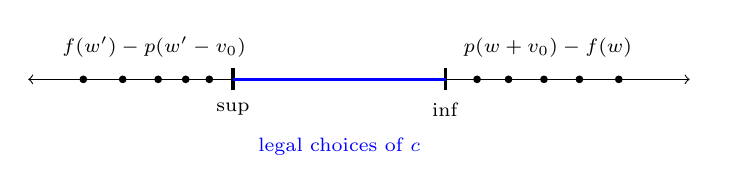
\begin{tikzpicture}[scale=1.0]
	\draw[<->] (-4.2,0) -- (4.2,0);
	\node[below right] at (4.2,0) {\small $\R$};
	% left cluster of values
	\foreach \x in {-3.5,-3.0,-2.55,-2.2,-1.9} { \fill (\x,0) circle (1.4pt); }
	\draw[very thick] (-1.6,-0.14) -- (-1.6,0.14);
	\node[below] at (-1.6,-0.18) {\scriptsize $\sup$};
	% right cluster of values
	\foreach \x in {1.5,1.9,2.35,2.8,3.3} { \fill (\x,0) circle (1.4pt); }
	\draw[very thick] (1.1,-0.14) -- (1.1,0.14);
	\node[below] at (1.1,-0.18) {\scriptsize $\inf$};
	% the window
	\draw[very thick, color=blue] (-1.6,0) -- (1.1,0);
	\node[color=blue, below] at (-0.25,-0.62) {\scriptsize legal choices of $c$};
	% labels for the clusters
	\node[above] at (-2.6,0.15) {\scriptsize $f(w') - p(w' - v_0)$};
	\node[above] at (2.4,0.15) {\scriptsize $p(w + v_0) - f(w)$};
\end{tikzpicture}
\end{center}

\begin{theorem}[Hahn--Banach, analytic form]
	Let $V$ be a real vector space, $p : V \to \R$ sublinear, $W \subseteq V$ a subspace and $f : W \to \R$ linear with $f(w) \leq p(w)$ for all $w \in W$. Then there is a linear $\wt f : V \to \R$ with $\wt f|_W = f$ and $\wt f(v) \leq p(v)$ for all $v \in V$.
\end{theorem}

\begin{proof}
	Let $P$ be the set of pairs $(U, g)$ where $W \subseteq U \subseteq V$ is a subspace, $g : U \to \R$ is linear, $g|_W = f$ and $g \leq p$ on $U$. Order $P$ by
	$$(U_1, g_1) \leq (U_2, g_2) \iff U_1 \subseteq U_2 \text{ and } g_2|_{U_1} = g_1.$$
	This is a partial order, and $P \neq \emptyset$ as $(W, f) \in P$.

	Let $\mathcal{C} = \{(U_i, g_i)\}_{i \in I}$ be a chain in $P$. Put $U = \bigcup_i U_i$ and define $g$ on $U$ by $g(u) = g_i(u)$ whenever $u \in U_i$; this is well defined by the compatibility built into the order. Since $\mathcal C$ is a chain, any two elements of $U$ lie in a common $U_i$, so $U$ is a subspace and $g$ is linear; and $g \leq p$ since each $g_i \leq p$. So $(U,g) \in P$ is an upper bound for $\mathcal{C}$.

	By Zorn's lemma, $P$ has a maximal element $(U_{\max}, \wt f)$. If $U_{\max} \neq V$, pick $v_0 \in V \setminus U_{\max}$ and apply the one-step extension lemma to obtain a strictly larger element of $P$, contradicting maximality. Hence $U_{\max} = V$.
\end{proof}

Notice that the picture of the extension is exactly a growing domain: we start on $W$, and repeatedly (transfinitely) enlarge the domain by one dimension, always keeping underneath the ceiling $p$.

\begin{center}
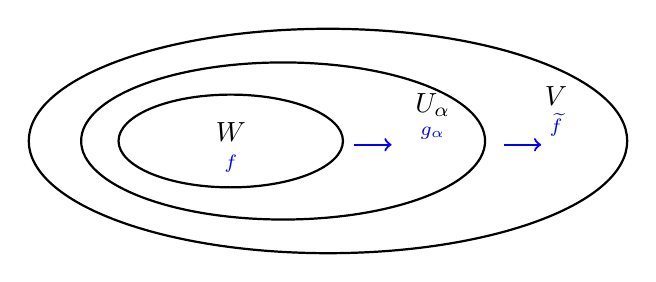
\begin{tikzpicture}[scale=0.95]
	% nested domains as nested ellipses
	\draw[thick] (0,0) ellipse (4 and 1.5);
	\draw[thick] (-0.6,0) ellipse (2.7 and 1.05);
	\draw[thick] (-1.3,0) ellipse (1.5 and 0.62);
	\node at (-1.3,0.12) {$W$};
	\node at (1.4,0.48) {$U_\alpha$};
	\node at (3.05,0.6) {$V$};
	\node[color=blue] at (-1.3,-0.3) {\scriptsize $f$};
	\node[color=blue] at (1.4,0.11) {\scriptsize $g_\alpha$};
	\node[color=blue] at (3.05,0.22) {\scriptsize $\wt f$};
	\draw[->, thick, color=blue] (0.35,-0.05) -- (0.85,-0.05);
	\draw[->, thick, color=blue] (2.35,-0.05) -- (2.85,-0.05);
\end{tikzpicture}
\end{center}

For the complex case, and for the applications we actually want, the following symmetric version is more convenient. Recall that a \vocab{seminorm} is a map $p : V \to [0,\infty)$ with $p(v+w) \leq p(v) + p(w)$ and $p(\lambda v) = |\lambda| p(v)$ for all scalars $\lambda$.

\begin{theorem}[Hahn--Banach, seminorm form]
	Let $V$ be a vector space over $\F = \R$ or $\C$, let $p$ be a seminorm on $V$, let $W \subseteq V$ be a subspace and let $f : W \to \F$ be linear with $|f(w)| \leq p(w)$ on $W$. Then there is a linear $\wt f : V \to \F$ with $\wt f|_W = f$ and $|\wt f(v)| \leq p(v)$ for all $v \in V$.
\end{theorem}

\begin{proof}
	\emph{Real case.} A seminorm is sublinear, so the analytic form gives an extension with $\wt f \leq p$. Then also $-\wt f(v) = \wt f(-v) \leq p(-v) = p(v)$, so $|\wt f| \leq p$.

	\emph{Complex case.} Let $g = \re f : W \to \R$, which is $\R$-linear, and note that
	$$f(w) = g(w) - i g(iw),$$
	since writing $f(w) = g(w) + ih(w)$ and using $f(iw) = if(w)$ gives $h(w) = -g(iw)$. Now $|g| \leq |f| \leq p$, and regarding $V$ as a real vector space, the real case gives an $\R$-linear extension $\wt g : V \to \R$ with $|\wt g| \leq p$. Define
	$$\wt f(v) = \wt g(v) - i \wt g(iv).$$
	This is $\R$-linear, and $\wt f(iv) = \wt g(iv) - i\wt g(-v) = i(\wt g(v) - i \wt g(iv)) = i \wt f(v)$, so it is $\C$-linear. It restricts to $f$ on $W$ by the identity above.

	Finally, fix $v$ and choose $\theta \in \R$ with $e^{i\theta} \wt f(v) = |\wt f(v)|$. Then
	$$|\wt f(v)| = \wt f(e^{i\theta} v) = \re \wt f(e^{i\theta}v) = \wt g(e^{i\theta} v) \leq p(e^{i\theta}v) = p(v),$$
	using that $|\wt f(v)|$ is real so equals its own real part.
\end{proof}

\subsection{Consequences}

Now we harvest. Everything in this subsection follows by applying Hahn--Banach with $p = \norm{\cdot}$ or a scaled version of it.

\begin{corollary}[Norm-preserving extension]
	Let $X$ be a normed space, $W \subseteq X$ a subspace and $f \in W^*$. Then there is $\wt f \in X^*$ with $\wt f|_W = f$ and $\norm{\wt f}_{X^*} = \norm{f}_{W^*}$.
\end{corollary}

\begin{proof}
	Apply the seminorm form with $p(x) = \norm{f}_{W^*}\norm{x}$, which is a seminorm (indeed a norm if $f \neq 0$) and dominates $|f|$ on $W$. We obtain $\wt f$ with $|\wt f(x)| \leq \norm{f}\norm{x}$, so $\norm{\wt f} \leq \norm{f}$; and $\norm{\wt f} \geq \norm{f}$ since $\wt f$ extends $f$.
\end{proof}

\begin{corollary}[Support functionals]
	Let $X$ be a normed space and $x_0 \in X$ with $x_0 \neq 0$. Then there is $f \in X^*$ with $\norm{f} = 1$ and $f(x_0) = \norm{x_0}$.
\end{corollary}

\begin{proof}
	Let $W = \F x_0$ and define $f_0(\lambda x_0) = \lambda \norm{x_0}$. Then $|f_0(\lambda x_0)| = \norm{\lambda x_0}$, so $\norm{f_0}_{W^*} = 1$. Extend by the previous corollary.
\end{proof}

Such an $f$ is called a \vocab{support functional} at $x_0$. It is the abstract version of `the tangent hyperplane to the unit ball at $x_0/\norm{x_0}$'.

\begin{corollary}
	Let $X$ be a normed space. Then:
	\begin{enumerate}[label=(\roman*)]
		\item if $X \neq \{0\}$ then $X^* \neq \{0\}$;
		\item $X^*$ separates points: if $x \neq y$ there is $f \in X^*$ with $f(x) \neq f(y)$;
		\item for every $x \in X$,
		$$\norm{x} = \sup \{ |f(x)| : f \in X^*, \ \norm{f} \leq 1 \},$$
		and the supremum is attained;
		\item the canonical embedding $\iota : X \to X^{**}$ is an isometry.
	\end{enumerate}
\end{corollary}

\begin{proof}
	(i) and (ii) follow from the existence of support functionals (for (ii) apply it to $x - y$). For (iii), the inequality $\leq$ is the support functional and $\geq$ is $|f(x)| \leq \norm{f}\norm{x}$. Finally (iv) is a restatement of (iii), since $\norm{\iota(x)} = \sup_{\norm{f}\leq 1}|\iota(x)(f)| = \sup_{\norm{f}\leq 1}|f(x)|$.
\end{proof}

Part (iv) is worth pausing on. It says that \emph{every normed space embeds isometrically into a Banach space}, namely the closure of $\iota(X)$ in $X^{**}$. This gives the slick construction of the completion promised earlier.

\begin{corollary}
	For $T \in \Bop(X,Y)$ we have $\norm{T^*} = \norm{T}$.
\end{corollary}

\begin{proof}
	We know $\norm{T^*} \leq \norm{T}$. Conversely, given $\varepsilon > 0$ pick $x$ with $\norm{x} \leq 1$ and $\norm{Tx} \geq \norm{T} - \varepsilon$, and let $f \in Y^*$ be a support functional at $Tx$, so $\norm{f}=1$ and $f(Tx) = \norm{Tx}$. Then
	$$\norm{T^*} \geq \norm{T^*f} \geq |(T^*f)(x)| = |f(Tx)| = \norm{Tx} \geq \norm{T} - \varepsilon. \qedhere$$
\end{proof}

\begin{corollary}[Separating a point from a subspace]
	Let $W \subseteq X$ be a closed subspace and $x_0 \in X \setminus W$. Then there is $f \in X^*$ with $\norm{f} = 1$, $f|_W = 0$ and $f(x_0) = \dist(x_0, W) > 0$.
\end{corollary}

\begin{proof}
	Work in the quotient $X/W$, which is a normed space since $W$ is closed, and let $q : X \to X/W$ be the quotient map, which satisfies $\norm{q} \leq 1$. As $x_0 \notin W$ we have $q(x_0) \neq 0$, so there is a support functional $g \in (X/W)^*$ with $\norm{g}=1$ and $g(q(x_0)) = \norm{q(x_0)} = \dist(x_0, W)$. Put $f = g \circ q$. Then $\norm{f} \leq 1$, $f$ kills $W$, and $f(x_0) = \dist(x_0,W)$. For $\norm{f} = 1$, note $\norm{f} \geq \dist(x_0,W)/\norm{x_0 - w}$ for every $w \in W$, and take the infimum over $w$.
\end{proof}

\begin{corollary}
	A subspace $W \subseteq X$ is dense if and only if the only $f \in X^*$ vanishing on $W$ is $f = 0$.
\end{corollary}

\begin{proof}
	If $W$ is dense and $f|_W = 0$ then $f = 0$ by continuity. Conversely if $\bar W \neq X$ pick $x_0 \notin \bar W$ and apply the previous corollary to the closed subspace $\bar W$.
\end{proof}

This last statement is one we will use again and again: to prove something lies in the closure of a subspace, it suffices to show every functional killing the subspace kills it too. It converts an approximation problem into a duality problem.

\begin{example}[Reflexivity of $\ell^p$]
	Let $1 < p < \infty$ and $q$ its conjugate. We computed $(\ell^p)^* \cong \ell^q$ and $(\ell^q)^* \cong \ell^p$, so $(\ell^p)^{**} \cong \ell^p$. Chasing the identifications shows the composite is exactly $\iota$, so $\ell^p$ is reflexive.

	On the other hand $c_0$ is not reflexive: $(c_0)^* \cong \ell^1$ and $(\ell^1)^* \cong \ell^\infty$, so $c_0^{**} \cong \ell^\infty \supsetneq c_0$. Nor is $\ell^1$ reflexive, since $(\ell^1)^{**} = (\ell^\infty)^*$ is strictly larger than $\ell^1$.
\end{example}

Hahn--Banach is not merely a device for extending functionals we already have; it can conjure up functionals with prescribed and rather magical properties. Here is the standard example.

\begin{example}[Banach limits]
	We construct a linear functional $\Lambda$ on the real space $\ell^\infty$ such that
	\begin{enumerate}[label=(\roman*)]
		\item $\liminf_n x_n \leq \Lambda(x) \leq \limsup_n x_n$ for every $x \in \ell^\infty$;
		\item $\Lambda(Lx) = \Lambda(x)$, where $L$ is the left shift.
	\end{enumerate}
	In particular $\Lambda$ agrees with $\lim$ on the convergent sequences, but is defined on \emph{all} bounded sequences, and is shift-invariant. So it assigns a `limit' to $(1,0,1,0,\dots)$ -- necessarily $\frac12$, by (i) and (ii) applied to $x + Lx = (1,1,1,\dots)$.

	For the construction, define
	$$p(x) = \lim_{n \to \infty}\ \sup_{k \geq 1} \frac{x_k + x_{k+1}+\cdots+x_{k+n-1}}{n}.$$
	The limit exists because the quantity $a_n = \sup_k(x_k + \cdots + x_{k+n-1})$ is subadditive in $n$, so $a_n/n$ converges by Fekete's lemma. One checks that $p$ is sublinear and that $p(x) \leq \limsup_n x_n$, with $p(Lx - x) \leq 0$ and $p(x - Lx)\leq 0$.

	Apply Hahn--Banach to the zero functional on the zero subspace, dominated by $p$: we get a linear $\Lambda \leq p$ on $\ell^\infty$. Then $\Lambda(x)\leq p(x)\leq\limsup x_n$, and $-\Lambda(x)=\Lambda(-x)\leq p(-x) \leq -\liminf x_n$, giving (i). And $\Lambda(Lx-x)\leq p(Lx-x)\leq0$ together with the same for $x - Lx$ gives (ii).

	Such a $\Lambda$ is called a \vocab{Banach limit}. It is an element of $(\ell^\infty)^*$ which does not come from $\ell^1$: it vanishes on $c_{00}$ but not on $\ell^\infty$. This is the promised proof that $(\ell^\infty)^* \supsetneq \ell^1$, and hence that $\ell^1$ is not reflexive.
\end{example}

\subsection{The Geometric Forms}

The analytic form is about functionals dominated by a sublinear $p$; the geometric form is about hyperplanes separating convex sets. The bridge between them is the following construction, which turns a convex set into a sublinear functional.

\begin{definition}[Minkowski functional]
	Let $V$ be a vector space and $C \subseteq V$ a convex set with $0 \in C$. The \vocab{Minkowski functional} (or \vocab{gauge}) of $C$ is
	$$\mu_C(v) = \inf \{ t > 0 : v \in tC \} \in [0, \infty].$$
\end{definition}

\begin{lemma}
	Let $X$ be a normed space and $C$ an open convex set with $0 \in C$. Then $\mu_C$ is sublinear, $C = \{v : \mu_C(v) < 1\}$, and there is $M > 0$ with $\mu_C(v) \leq M \norm{v}$.
\end{lemma}

\begin{proof}
	Positive homogeneity is immediate from the definition. For subadditivity, suppose $v \in sC$ and $w \in tC$, say $v = sc_1$, $w = tc_2$ with $c_i \in C$. Then
	$$\frac{v+w}{s+t} = \frac{s}{s+t}c_1 + \frac{t}{s+t}c_2 \in C$$
	by convexity, so $\mu_C(v+w) \leq s + t$; taking infima gives $\mu_C(v+w) \leq \mu_C(v) + \mu_C(w)$.

	Since $C$ is open and $0 \in C$, there is $r > 0$ with $B(0,r) \subseteq C$, whence $\mu_C(v) \leq \norm{v}/r$; take $M = 1/r$. If $v \in C$ then by openness $(1+\varepsilon)v \in C$ for small $\varepsilon$, so $\mu_C(v) \leq (1+\varepsilon)^{-1} < 1$; conversely $\mu_C(v) < 1$ gives $v \in tC \subseteq C$ for some $t < 1$ (using $0 \in C$ and convexity).
\end{proof}

\begin{theorem}[Hahn--Banach, separation form]
	Let $X$ be a real normed space and let $A, B \subseteq X$ be non-empty disjoint convex sets.
	\begin{enumerate}[label=(\roman*)]
		\item If $A$ is open, there exist $f \in X^* \setminus \{0\}$ and $\alpha \in \R$ with
		$$f(a) < \alpha \leq f(b) \qquad \text{for all } a \in A, \ b \in B.$$
		\item If $A$ is closed and $B$ is compact, there exist $f \in X^*\setminus\{0\}$ and $\alpha_1 < \alpha_2$ with
		$$f(a) \leq \alpha_1 < \alpha_2 \leq f(b) \qquad \text{for all } a \in A, \ b \in B.$$
	\end{enumerate}
\end{theorem}

\begin{proof}
	(i) Fix $a_0 \in A$, $b_0 \in B$ and set $v_0 = b_0 - a_0$ and
	$$C = A - B + v_0 = \{a - b + v_0 : a \in A, b \in B\}.$$
	Then $C$ is convex (a sum of convex sets), open (a union of translates of the open set $A$), and contains $0$ (take $a = a_0, b = b_0$). Also $v_0 \notin C$: otherwise $v_0 = a - b + v_0$ for some $a \in A, b\in B$, forcing $a = b$, contradicting disjointness.

	Let $\mu = \mu_C$, which is sublinear and bounded by $M\norm{\cdot}$. On the line $W = \R v_0$ define $g(t v_0) = t$. For $t > 0$ we have $g(tv_0) = t \leq t\mu(v_0) = \mu(tv_0)$, since $\mu(v_0) \geq 1$ as $v_0 \notin C$; for $t \leq 0$, $g(tv_0) \leq 0 \leq \mu(tv_0)$. So $g \leq \mu$ on $W$, and Hahn--Banach gives a linear $f : X \to \R$ with $f \leq \mu$ and $f(v_0) = 1$. Since $f(x) \leq \mu(x) \leq M\norm{x}$ and $-f(x) = f(-x) \leq M\norm{x}$, we get $f \in X^*$, and $f \neq 0$.

	Now for $a \in A$, $b \in B$, the point $a - b + v_0 \in C$ so $\mu(a - b + v_0) < 1$, giving
	$$f(a) - f(b) + 1 = f(a - b + v_0) \leq \mu(a-b+v_0) < 1,$$
	i.e.\ $f(a) < f(b)$. Hence $\alpha := \inf_{b \in B} f(b)$ satisfies $f(a) \leq \alpha \leq f(b)$ for all $a, b$. Finally $f(a) < \alpha$ strictly: $A$ is open and $f \neq 0$, so $f(A)$ is an open subset of $\R$ (pick $u$ with $f(u) = 1$; then $f(a + su) = f(a) + s$ covers a neighbourhood of $f(a)$), and an open set cannot contain its own supremum.

	(ii) Since $A$ is closed, $B$ compact and $A \cap B = \emptyset$, the distance $\delta = \dist(A,B)$ is strictly positive. (If $\dist(a_n,b_n) \to 0$, pass to a convergent subsequence $b_n \to b \in B$; then $a_n \to b$, so $b \in \bar A = A$, a contradiction.) Let
	$$A_\delta = A + B(0, \delta/2),$$
	which is open and convex, and disjoint from $B$ by the choice of $\delta$. By (i) there is $f \neq 0$ with $f(a') < f(b)$ for $a' \in A_\delta$, $b \in B$. For $a \in A$ and $\norm{u} < \delta/2$ we get $f(a) + f(u) < f(b)$, and taking the supremum over such $u$ gives
	$$f(a) + \tfrac{\delta}{2}\norm{f} \leq f(b)$$
	for all $a \in A, b \in B$. As $\norm{f} > 0$ we may take $\alpha_1 = \sup_A f$ and $\alpha_2 = \alpha_1 + \frac{\delta}{2}\norm{f} > \alpha_1$.
\end{proof}

Geometrically, a functional $f$ and a level $\alpha$ determine an affine \vocab{hyperplane} $H = f^{-1}(\alpha)$, which is closed exactly when $f$ is continuous, and which divides $X$ into two half-spaces $\{f < \alpha\}$ and $\{f > \alpha\}$. The theorem says that two disjoint convex sets can be put on opposite sides of a hyperplane, strictly so if one is closed and the other compact.

\begin{center}
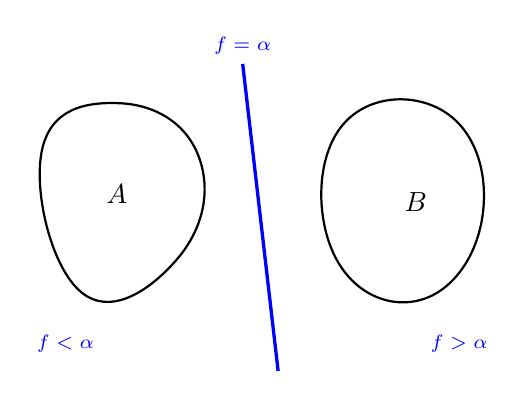
\begin{tikzpicture}[scale=1.0]
	% convex set A (blob on the left)
	\draw[thick] plot[smooth cycle, tension=0.8] coordinates {(-2.9,0.9) (-1.9,1.5) (-0.9,0.8) (-1.2,-0.5) (-2.4,-0.9)};
	\node at (-1.95,0.35) {$A$};
	% convex set B (blob on the right)
	\draw[thick] plot[smooth cycle, tension=0.8] coordinates {(0.9,1.2) (2.2,1.4) (2.7,0.1) (1.9,-1.0) (0.8,-0.4)};
	\node at (1.85,0.25) {$B$};
	% separating hyperplane
	\draw[very thick, color=blue] (0.1,-1.9) -- (-0.35,2.0);
	\node[color=blue, above] at (-0.35,2.0) {\scriptsize $f = \alpha$};
	\node[color=blue] at (-2.6,-1.55) {\scriptsize $f < \alpha$};
	\node[color=blue] at (2.4,-1.55) {\scriptsize $f > \alpha$};
\end{tikzpicture}
\end{center}

\begin{corollary}
	Let $X$ be a real normed space, $C \subseteq X$ a closed convex set and $x_0 \notin C$. Then there is $f \in X^*$ with $\sup_{c \in C} f(c) < f(x_0)$. In particular, a closed convex set is the intersection of the closed half-spaces containing it.
\end{corollary}

\begin{proof}
	Apply part (ii) with $A = C$ and $B = \{x_0\}$, which is compact. The final statement follows since any $x_0 \notin C$ is excluded by one of these half-spaces.
\end{proof}

\begin{remark}
	Convexity is essential. In $\R^2$ we cannot separate a point at the centre of an annulus from the annulus itself. The theorem is a genuinely convex-geometric statement, and it is the starting point of convex analysis and of the theory of weak topologies.
\end{remark}

\section{The Baire Category Theorem}

The Hahn--Banach theorem was a statement about the algebraic and convex structure of a normed space, and its proof used no completeness at all. We now turn to the other pillar of the subject, which is entirely about completeness, and which is in some ways even more remarkable: a very soft topological statement whose consequences include three of the fundamental theorems of functional analysis.

\subsection{Category}

Recall that a subset $A$ of a topological space $X$ is \vocab{dense} if $\bar A = X$, equivalently if $A$ meets every non-empty open set.

\begin{definition}[Nowhere dense]
	A subset $A$ of a topological space $X$ is \vocab{nowhere dense} (or \vocab{rare}) if $\bar A$ has empty interior, i.e.\ $\bar A$ contains no non-empty open set.
\end{definition}

Equivalently, $A$ is nowhere dense if and only if $X \setminus \bar A$ is dense: every open set contains an open subset missing $A$ entirely. Think of it as being `full of holes at every scale'.

\begin{example}
	\begin{enumerate}[label=(\roman*)]
		\item A single point in $\R$ is nowhere dense, as is any finite set, as is $\{1/n : n \in \N\} \cup \{0\}$.
		\item $\Z$ is nowhere dense in $\R$, but $\Q$ is \emph{not} -- its closure is all of $\R$.
		\item The Cantor set is nowhere dense in $[0,1]$: it is closed, and contains no interval since it has empty interior by construction.
		\item In $C[0,1]$, the set of polynomials of degree at most $d$ is nowhere dense (it is a finite-dimensional, hence closed, proper subspace, and a proper subspace has empty interior -- if it contained a ball it would contain a translate of a ball about $0$, hence everything).
	\end{enumerate}
\end{example}

\begin{center}
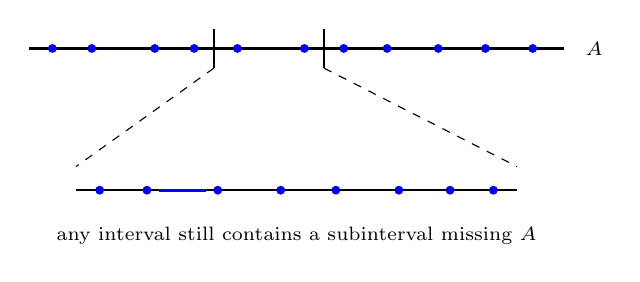
\begin{tikzpicture}[scale=1.0]
	% a nowhere dense set drawn as scattered thickened points on a line, with a magnified window
	\draw[thick] (-4.2,0.9) -- (2.6,0.9);
	\foreach \x in {-3.9,-3.4,-2.6,-2.1,-1.55,-0.7,-0.2,0.35,1.0,1.6,2.2} {
		\fill[color=blue] (\x,0.9) circle (1.6pt);
	}
	\node[right] at (2.75,0.9) {\scriptsize $A$};
	% window brackets
	\draw[thick] (-1.85,1.15) -- (-1.85,0.65);
	\draw[thick] (-0.45,1.15) -- (-0.45,0.65);
	% zoom lines
	\draw[dashed] (-1.85,0.65) -- (-3.6,-0.6);
	\draw[dashed] (-0.45,0.65) -- (2.0,-0.6);
	% magnified copy
	\draw[thick] (-3.6,-0.9) -- (2.0,-0.9);
	\foreach \x in {-3.3,-2.7,-1.8,-1.0,-0.3,0.5,1.15,1.7} {
		\fill[color=blue] (\x,-0.9) circle (1.6pt);
	}
	\node[below] at (-0.8,-1.25) {\scriptsize any interval still contains a subinterval missing $A$};
	\draw[very thick, color=blue] (-2.55,-0.9) -- (-1.95,-0.9);
\end{tikzpicture}
\end{center}

\begin{definition}[Meagre]
	A subset of a topological space is \vocab{meagre} (or \vocab{of first category}) if it is a countable union of nowhere dense sets, and \vocab{of second category} otherwise. A set whose complement is meagre is called \vocab{residual} or \vocab{comeagre}.
\end{definition}

`Meagre' is a topological notion of smallness. It behaves as one would hope: a countable union of meagre sets is meagre, and a subset of a meagre set is meagre. The content of the Baire category theorem is that in a complete space, `meagre' really does mean small -- in particular, the whole space is not meagre in itself.

\begin{theorem}[Baire Category Theorem]
	Let $(X,d)$ be a complete non-empty metric space. Then:
	\begin{enumerate}[label=(\roman*)]
		\item if $(U_n)_{n \geq 1}$ are open and dense in $X$, then $\bigcap_{n \geq 1} U_n$ is dense in $X$;
		\item $X$ is not meagre in itself. Equivalently, if $X = \bigcup_{n\geq 1} F_n$ with each $F_n$ closed, then some $F_n$ has non-empty interior.
	\end{enumerate}
\end{theorem}

\begin{proof}
	(i) Let $W \subseteq X$ be non-empty and open; we must show $W \cap \bigcap_n U_n \neq \emptyset$. We construct a nested sequence of closed balls.

	Since $U_1$ is dense and open, $W \cap U_1$ is non-empty and open, so it contains a closed ball $\bar B(x_1, r_1)$ with $0 < r_1 < 1$. Inductively, given $\bar{B}(x_n, r_n)$, the set $B(x_n, r_n) \cap U_{n+1}$ is non-empty (density of $U_{n+1}$) and open, so it contains a closed ball $\bar B(x_{n+1}, r_{n+1})$ with $0 < r_{n+1} < 2^{-n}$.

	By construction $\bar B(x_1,r_1) \supseteq \bar B(x_2,r_2) \supseteq \cdots$ and $r_n \to 0$. For $m > n$ we have $x_m \in \bar B(x_n, r_n)$, so $d(x_n, x_m) \leq r_n \to 0$ and $(x_n)$ is Cauchy. By completeness $x_n \to x$ for some $x \in X$, and since $x_m \in \bar B(x_n, r_n)$ for all $m \geq n$ and this ball is closed, $x \in \bar B(x_n, r_n)$ for every $n$. Hence
	$$x \in \bar B(x_1, r_1) \subseteq W \cap U_1 \quad \text{and} \quad x \in \bar B(x_{n+1},r_{n+1}) \subseteq U_{n+1}$$
	for every $n$, so $x \in W \cap \bigcap_n U_n$ as required.

	(ii) Suppose $X = \bigcup_n A_n$ with each $A_n$ nowhere dense. Then $U_n = X \setminus \bar{A_n}$ is open and dense, and $\bigcap_n U_n = X \setminus \bigcup_n \bar{A_n} = \emptyset$, contradicting (i) (as $X \neq \emptyset$). The reformulation follows by taking $F_n$ closed with empty interior, i.e.\ nowhere dense.
\end{proof}

\begin{center}
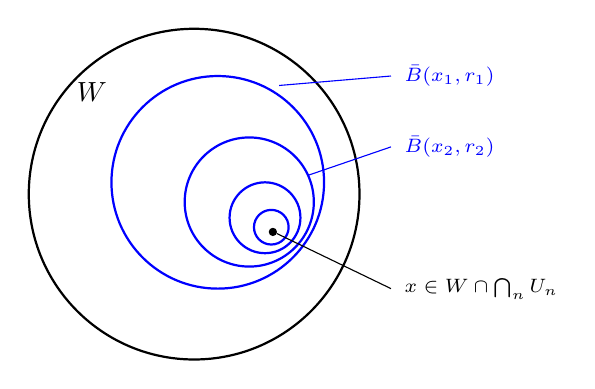
\begin{tikzpicture}[scale=1.0]
	\draw[thick] (0,0) circle (2.1);
	\node at (-1.3,1.3) {$W$};
	\draw[thick, color=blue] (0.3,0.15) circle (1.35);
	\draw[thick, color=blue] (0.7,-0.1) circle (0.82);
	\draw[thick, color=blue] (0.9,-0.3) circle (0.45);
	\draw[thick, color=blue] (0.98,-0.42) circle (0.22);
	\fill (1.0,-0.48) circle (1.5pt);
	% leader lines out to the right
	\draw[color=blue] (1.08,1.38) -- (2.5,1.5);
	\node[color=blue, right] at (2.55,1.5) {\scriptsize $\bar B(x_1,r_1)$};
	\draw[color=blue] (1.45,0.24) -- (2.5,0.6);
	\node[color=blue, right] at (2.55,0.6) {\scriptsize $\bar B(x_2,r_2)$};
	\draw (1.05,-0.5) -- (2.5,-1.2);
	\node[right] at (2.55,-1.2) {\scriptsize $x \in W \cap \bigcap_n U_n$};
\end{tikzpicture}
\end{center}

Before the big applications, here are two quick ones that show the flavour.

\begin{proposition}
	$\Q$ is not the intersection of countably many open subsets of $\R$.
\end{proposition}

\begin{proof}
	Suppose $\Q = \bigcap_n U_n$ with $U_n$ open. Each $U_n \supseteq \Q$ is dense. Enumerate $\Q = \{q_1, q_2, \dots\}$; then each $V_n = \R \setminus \{q_n\}$ is open and dense. So
	$$\bigcap_n U_n \cap \bigcap_n V_n = \Q \setminus \Q = \emptyset,$$
	contradicting Baire applied to the complete space $\R$.
\end{proof}

\begin{proposition}
	An infinite-dimensional Banach space cannot have a countable Hamel basis.
\end{proposition}

\begin{proof}
	Suppose $X$ has Hamel basis $\{e_1, e_2, \dots\}$, and let $X_n = \spn\{e_1,\dots,e_n\}$. Each $X_n$ is finite-dimensional, hence closed, and proper (as $X$ is infinite-dimensional), hence has empty interior. But $X = \bigcup_n X_n$, contradicting Baire.
\end{proof}

\begin{remark}
	Hence, for instance, $c_{00}$ (which \emph{does} have the countable Hamel basis $\{e_n\}$) admits no norm making it complete. That is a strong statement, and it would be painful to prove directly.
\end{remark}

\begin{theorem}[Osgood]
	Let $X$ be a complete metric space and $f_n : X \to \R$ continuous with $f_n \to f$ pointwise. Then the set of points at which $f$ is continuous is residual, in particular dense.
\end{theorem}

\begin{proof}
	For $\varepsilon>0$ and $N \in \N$ put
	$$F_{N,\varepsilon} = \{ x \in X : |f_n(x)-f_m(x)|\leq\varepsilon \text{ for all } n,m\geq N\},$$
	which is closed by continuity of the $f_n$. Pointwise convergence gives $X = \bigcup_N F_{N,\varepsilon}$, so
	$$U_\varepsilon = \bigcup_N \operatorname{int} F_{N,\varepsilon}$$
	is open, and it is dense: for any open ball $B$, applying Baire inside the complete space $\bar B$ to the sets $F_{N,\varepsilon}\cap\bar B$ produces some $N$ for which $F_{N,\varepsilon}\cap\bar B$ has interior, so $U_\varepsilon$ meets $B$.

	Now let $D = \bigcap_{k\geq1}U_{1/k}$, a residual set. We claim $f$ is continuous at each $x \in D$. Given $\varepsilon>0$ choose $k$ with $3/k<\varepsilon$. As $x \in U_{1/k}$, there is $N$ and an open $V \ni x$ with $V \subseteq F_{N,1/k}$. Letting $m \to\infty$ in the defining inequality gives $|f_N(y)-f(y)|\leq 1/k$ for all $y \in V$. Shrinking $V$ so that $|f_N(y)-f_N(x)|<1/k$ on it, we get
	$$|f(y)-f(x)| \leq |f(y)-f_N(y)|+|f_N(y)-f_N(x)|+|f_N(x)-f(x)| \leq \frac{3}{k}<\varepsilon. \qedhere$$
\end{proof}

So a pointwise limit of continuous functions, while not continuous in general, cannot be discontinuous everywhere -- which incidentally shows that the indicator of $\Q$ is not a pointwise limit of continuous functions, though it is a pointwise limit of pointwise limits.

\subsection{A Continuous Nowhere Differentiable Function}

Here is the classical showpiece application. Weierstrass constructed such a function explicitly in 1872, to general consternation; Banach observed in 1931 that Baire category makes the existence almost obvious -- and in fact shows that such functions are the \emph{typical} continuous function, the differentiable ones forming a meagre set.

\begin{theorem}
	There is a continuous function $f : [0,1] \to \R$ which is differentiable at no point of $[0,1]$. Indeed, the set of such $f$ is residual in $C[0,1]$.
\end{theorem}

\begin{proof}
	Work in the Banach space $X = C[0,1]$ with the sup norm. For $n \in \N$ let
	$$A_n = \left\{ f \in X : \exists\, x \in [0,1] \text{ with } |f(x) - f(y)| \leq n|x-y| \ \text{for all } y \in [0,1] \right\}.$$
	If $f$ is differentiable at some point $x$, then $f$ is Lipschitz at $x$ in this sense with some constant, so $f \in A_n$ for some $n$. Thus it suffices to show each $A_n$ is closed with empty interior; then $\bigcup_n A_n$ is meagre and any $f$ in its (non-empty, by Baire) complement works.

	\emph{$A_n$ is closed.} Let $f_k \in A_n$ with $f_k \to f$ uniformly, and let $x_k$ witness $f_k \in A_n$. By compactness of $[0,1]$, pass to a subsequence with $x_k \to x$. For any $y \in [0,1]$,
	$$|f(x) - f(y)| \leq |f(x) - f(x_k)| + |f(x_k) - f_k(x_k)| + |f_k(x_k) - f_k(y)| + |f_k(y) - f(y)|.$$
	The second and fourth terms are at most $\norm{f - f_k}_\infty \to 0$; the first tends to $0$ by continuity of $f$ and $x_k \to x$; and the third is at most $n|x_k - y| \to n|x - y|$. Hence $|f(x)-f(y)| \leq n|x-y|$, so $f \in A_n$.

	\emph{$A_n$ has empty interior.} Let $f \in X$ and $\varepsilon > 0$; we find $g$ with $\norm{f - g}_\infty < \varepsilon$ and $g \notin A_n$. By the Weierstrass approximation theorem (or just uniform continuity and piecewise-linear interpolation), choose a piecewise linear $h$ with $\norm{f - h}_\infty < \varepsilon/2$. Let $M$ be the maximum absolute slope of $h$. Let $s$ be a `sawtooth' function of amplitude $\varepsilon/2$ whose slopes all have absolute value $\Lambda$, where $\Lambda > M + n$; explicitly, $s$ is the $\varepsilon/2$-scaled zigzag of period $\varepsilon/\Lambda$. Put $g = h + s$.

	Then $\norm{f - g}_\infty \leq \norm{f-h}_\infty + \norm{s}_\infty < \varepsilon$. At every point $x$, and for $y$ close enough to $x$ on a suitable side, the difference quotient of $g$ has absolute value at least $\Lambda - M > n$, since $s$ contributes slope $\pm \Lambda$ and $h$ at most $M$. Hence $g \notin A_n$.
\end{proof}

\begin{center}
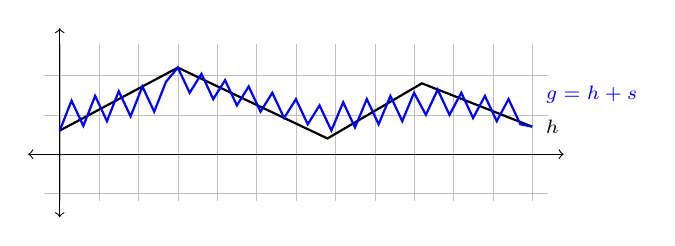
\begin{tikzpicture}[scale=1.0]
	\draw[ultra thin, color=lightgray, step=0.5] (-0.2,-0.6) grid (6.2,1.4);
	\draw[<->] (-0.4,0) -- (6.4,0);
	\draw[<->] (0,-0.8) -- (0,1.6);
	% piecewise linear h
	\draw[thick] (0,0.3) -- (1.5,1.1) -- (3.4,0.2) -- (4.6,0.9) -- (6,0.35);
	\node[right] at (6.05,0.35) {\scriptsize $h$};
	% h + sawtooth
	\draw[thick, color=blue]
		(0,0.3) -- (0.15,0.68) -- (0.3,0.36) -- (0.45,0.74) -- (0.6,0.42) -- (0.75,0.8) -- (0.9,0.48)
		-- (1.05,0.86) -- (1.2,0.54) -- (1.35,0.92) -- (1.5,1.1) -- (1.65,0.78) -- (1.8,1.02) -- (1.95,0.7)
		-- (2.1,0.94) -- (2.25,0.62) -- (2.4,0.86) -- (2.55,0.54) -- (2.7,0.78) -- (2.85,0.46)
		-- (3.0,0.7) -- (3.15,0.38) -- (3.3,0.62) -- (3.45,0.3) -- (3.6,0.66) -- (3.75,0.34)
		-- (3.9,0.7) -- (4.05,0.38) -- (4.2,0.74) -- (4.35,0.42) -- (4.5,0.78) -- (4.65,0.5)
		-- (4.8,0.82) -- (4.95,0.5) -- (5.1,0.78) -- (5.25,0.46) -- (5.4,0.74) -- (5.55,0.42)
		-- (5.7,0.7) -- (5.85,0.38) -- (6,0.35);
	\node[color=blue, right] at (6.05,0.75) {\scriptsize $g = h + s$};
\end{tikzpicture}
\end{center}

The picture is the point of the proof: adding a tiny but very steep sawtooth changes the function hardly at all in the uniform norm, while destroying any chance of a bounded difference quotient. Uniform closeness is simply blind to derivatives.

\subsection{The Principle of Uniform Boundedness}

The second application is the one that gets used most often in practice.

\begin{theorem}[Banach--Steinhaus / Uniform Boundedness Principle]
	Let $X$ be a Banach space, $Y$ a normed space, and $\{T_i\}_{i \in I} \subseteq \Bop(X,Y)$ a family of bounded operators which is \emph{pointwise bounded}:
	$$\sup_{i \in I} \norm{T_i x} < \infty \qquad \text{for every } x \in X.$$
	Then it is \emph{uniformly bounded}: $\sup_{i \in I} \norm{T_i} < \infty$.
\end{theorem}

\begin{proof}
	For $n \in \N$ let
	$$F_n = \{ x \in X : \norm{T_i x} \leq n \text{ for all } i \in I \} = \bigcap_{i \in I} \{x : \norm{T_ix} \leq n\}.$$
	Each set in the intersection is closed (preimage of a closed set under the continuous map $x \mapsto \norm{T_i x}$), so $F_n$ is closed. By pointwise boundedness $X = \bigcup_n F_n$.

	Since $X$ is complete, Baire gives some $N$ with $F_N$ having non-empty interior, say $\bar B(x_0, r) \subseteq F_N$ with $r > 0$. Now for any $x$ with $\norm{x} \leq 1$ and any $i$,
	$$\norm{T_i x} = \frac{1}{r}\norm{T_i (x_0 + rx) - T_i x_0} \leq \frac{1}{r}\left( \norm{T_i(x_0+rx)} + \norm{T_ix_0} \right) \leq \frac{2N}{r},$$
	since both $x_0 + rx$ and $x_0$ lie in $\bar B(x_0,r) \subseteq F_N$. Hence $\norm{T_i} \leq 2N/r$ for all $i$.
\end{proof}

The theorem is genuinely surprising: pointwise information about a family of operators upgrades, for free, to uniform information. Completeness of $X$ is essential -- on $c_{00}$, the functionals $f_n(x) = n x_n$ are pointwise bounded but have $\norm{f_n} = n$.

\begin{corollary}
	Let $X$ be a Banach space, $Y$ a normed space and $T_n \in \Bop(X,Y)$ with $T_n x \to Tx$ for every $x \in X$. Then $T$ is linear and bounded, with
	$$\norm{T} \leq \liminf_{n} \norm{T_n} < \infty.$$
\end{corollary}

\begin{proof}
	Linearity is clear. Each convergent sequence $(T_nx)$ is bounded, so $\{T_n\}$ is pointwise bounded, hence $\sup_n \norm{T_n} = M < \infty$ by uniform boundedness. Then $\norm{Tx} = \lim \norm{T_nx} \leq M\norm{x}$. The sharper bound follows by taking a subsequence realising the $\liminf$.
\end{proof}

\begin{corollary}[Weak boundedness implies boundedness]
	Let $X$ be a normed space and $S \subseteq X$. If $f(S)$ is bounded in $\F$ for every $f \in X^*$, then $S$ is bounded in norm.
\end{corollary}

\begin{proof}
	Apply uniform boundedness in the Banach space $X^*$ to the family $\{\iota(x) : x \in S\} \subseteq X^{**}$. The hypothesis says exactly that this family is pointwise bounded on $X^*$, so $\sup_{x \in S}\norm{\iota(x)} < \infty$; and $\norm{\iota(x)} = \norm{x}$ by Hahn--Banach.
\end{proof}

Note the slight sleight of hand: $X$ itself need not be complete, but $X^*$ always is, so we may apply Baire there. This trick -- move the problem into a dual space to gain completeness -- is worth remembering.

\begin{example}[Divergence of Fourier series]
	Here is a striking application. For $f \in C(\mathbb{T})$, the continuous $2\pi$-periodic functions with the sup norm, write
	$$S_N f(x) = \sum_{|k| \leq N} \hat f(k) e^{ikx}, \qquad \hat f(k) = \frac{1}{2\pi}\int_{-\pi}^{\pi} f(t)e^{-ikt}\dd t.$$
	We claim that there is a continuous function whose Fourier series diverges at $0$; indeed the set of such functions is residual.

	Consider the functionals $\Lambda_N : C(\mathbb{T}) \to \C$, $\Lambda_N f = S_Nf(0)$. A computation with the geometric series gives
	$$\Lambda_N f = \frac{1}{2\pi}\int_{-\pi}^\pi f(t) D_N(t) \dd t, \qquad D_N(t) = \sum_{|k|\leq N}e^{-ikt} = \frac{\sin\big((N+\frac12)t\big)}{\sin(t/2)},$$
	where $D_N$ is the \vocab{Dirichlet kernel}. One checks that
	$$\norm{\Lambda_N} = \frac{1}{2\pi}\int_{-\pi}^{\pi}|D_N(t)|\dd t =: L_N,$$
	the \vocab{Lebesgue constant}: the bound $\leq$ is clear, and it is attained in the limit by taking $f$ to approximate $\sgn D_N$ continuously. Now
	$$L_N \geq \frac{1}{\pi}\int_0^{\pi} \frac{|\sin((N+\frac12)t)|}{t}\dd t \geq \frac{1}{\pi}\sum_{k=1}^{N}\frac{1}{k}\int_{0}^{\pi}|\sin u| \frac{\dd u}{\pi} \cdot c \longrightarrow \infty$$
	for a suitable constant $c > 0$; the essential point is the divergence of the harmonic series, giving $L_N \sim \frac{4}{\pi^2}\log N$.

	So $\norm{\Lambda_N} \to \infty$. Since $C(\mathbb{T})$ is a Banach space, uniform boundedness says the family $\{\Lambda_N\}$ cannot be pointwise bounded: there is $f \in C(\mathbb{T})$ with $\sup_N |S_Nf(0)| = \infty$, so the Fourier series of $f$ diverges at $0$.
\end{example}

\begin{remark}
	This example is worth contrasting with what happens in $L^2$, where we will prove that the Fourier series of \emph{every} function converges (in the $L^2$ norm). Pointwise convergence is a much more delicate matter; Carleson proved in 1966 that the Fourier series of an $L^2$ function converges almost everywhere, which is a very deep theorem.
\end{remark}

\subsection{The Open Mapping Theorem}

Recall that a map $T : X \to Y$ is \vocab{open} if $T(U)$ is open in $Y$ whenever $U$ is open in $X$. This is a strong requirement, but for surjective bounded operators between Banach spaces it comes for free.

\begin{theorem}[Open Mapping Theorem]
	Let $X, Y$ be Banach spaces and $T \in \Bop(X,Y)$ surjective. Then $T$ is an open map. Equivalently, there is $c > 0$ with
	$$T(B_X) \supseteq c B_Y,$$
	where $B_X, B_Y$ are the open unit balls.
\end{theorem}

\begin{proof}
	First, the equivalence. If $T(B_X) \supseteq cB_Y$ then for $U \subseteq X$ open and $x \in U$, choose $r$ with $x + rB_X \subseteq U$; then
	$$T(U) \supseteq Tx + rT(B_X) \supseteq Tx + rcB_Y,$$
	so $T(U)$ is open. Conversely if $T$ is open then $T(B_X)$ is an open set containing $0$.

	\emph{Step 1: $\overline{T(B_X)}$ contains a ball about $0$.} Since $T$ is surjective and $X = \bigcup_n nB_X$,
	$$Y = \bigcup_{n=1}^\infty T(nB_X) = \bigcup_{n=1}^\infty n\, T(B_X) \subseteq \bigcup_{n=1}^\infty n\,\overline{T(B_X)}.$$
	As $Y$ is complete, Baire gives an $n$ for which $n\overline{T(B_X)}$ has non-empty interior, hence so does $K := \overline{T(B_X)}$: say $B(y_0, r) \subseteq K$. Now $K$ is convex and symmetric ($-K = K$), being the closure of the convex symmetric set $T(B_X)$. So $B(-y_0,r) = -B(y_0,r) \subseteq K$, and for $\norm{y} < r$,
	$$y = \tfrac12\big((y_0 + y) + (-y_0 + y)\big) \in \tfrac12(K + K) = K$$
	by convexity. Hence $rB_Y \subseteq \overline{T(B_X)}$.

	\emph{Step 2: removing the closure.} We claim $\frac{r}{2}B_Y \subseteq T(B_X)$. By scaling, Step 1 gives
	$$2^{-k} r B_Y \subseteq \overline{T(2^{-k}B_X)} \qquad \text{for all } k \geq 0.$$
	Let $y \in Y$ with $\norm{y} < r/2$. Since $y \in \overline{T(\frac12 B_X)}$, there is $x_1$ with $\norm{x_1} < \frac12$ and $\norm{y - Tx_1} < r/4$. Since $y - Tx_1 \in \overline{T(\frac14 B_X)}$, there is $x_2$ with $\norm{x_2} < \frac14$ and $\norm{y - Tx_1 - Tx_2} < r/8$. Continuing, we obtain $x_k$ with $\norm{x_k} < 2^{-k}$ and
	$$\left\| y - T\left(\sum_{k=1}^n x_k\right) \right\| < 2^{-(n+1)}r.$$
	Now $\sum_k \norm{x_k} < 1$, so by completeness of $X$ the series $\sum_k x_k$ converges to some $x$ with $\norm{x} < 1$, and by continuity of $T$ we get $Tx = y$. Hence $y \in T(B_X)$.
\end{proof}

Both completeness hypotheses are used, and both are needed: completeness of $Y$ for Baire in Step 1, completeness of $X$ for the series in Step 2.

\begin{theorem}[Inverse Mapping Theorem]
	Let $X, Y$ be Banach spaces and $T \in \Bop(X,Y)$ a bijection. Then $T^{-1} \in \Bop(Y,X)$; that is, $T$ is an isomorphism.
\end{theorem}

\begin{proof}
	$T$ is open by the open mapping theorem, and an open bijection has continuous inverse: $(T^{-1})^{-1}(U) = T(U)$ is open for every open $U$.
\end{proof}

This is a genuinely useful tool. It says that for operators between Banach spaces, algebraic invertibility automatically gives topological invertibility -- so to check that an equation $Tx = y$ has a solution depending continuously on the data, we need only check existence and uniqueness.

\begin{corollary}
	Let $\norm{\cdot}_1$ and $\norm{\cdot}_2$ be two norms on a vector space $X$, each making $X$ complete. If there is $C$ with $\norm{x}_2 \leq C\norm{x}_1$ for all $x$, then the norms are equivalent.
\end{corollary}

\begin{proof}
	The identity map $(X, \norm{\cdot}_1) \to (X, \norm{\cdot}_2)$ is a bounded bijection between Banach spaces, hence has bounded inverse.
\end{proof}

\begin{corollary}
	Let $X$ be a Banach space and $X = Y \oplus Z$ an algebraic direct sum with $Y, Z$ closed subspaces. Then the projection $P : X \to Y$ along $Z$ is bounded.
\end{corollary}

\begin{proof}
	$Y \oplus Z$ with the norm $\norm{(y,z)} = \norm{y} + \norm{z}$ is a Banach space (as $Y, Z$ are closed in the complete $X$), and the addition map $(y,z) \mapsto y+z$ is a bounded bijection onto $X$. Its inverse $x \mapsto (Px, x - Px)$ is bounded by the inverse mapping theorem, so $P$ is bounded.
\end{proof}

\subsection{The Closed Graph Theorem}

To prove an operator is bounded we must show $x_n \to x$ implies $Tx_n \to Tx$. The closed graph theorem says that -- between Banach spaces -- we may \emph{assume} that $Tx_n$ converges, and only check that its limit is right. In practice this halves the work.

\begin{definition}[Graph]
	Let $T : X \to Y$ be linear. Its \vocab{graph} is
	$$\Gamma(T) = \{ (x, Tx) : x \in X \} \subseteq X \oplus Y.$$
	We say $T$ is \vocab{closed} if $\Gamma(T)$ is a closed subspace of $X \oplus Y$ (with the norm $\norm{(x,y)} = \norm{x} + \norm{y}$).
\end{definition}

Unwinding the definition, $T$ is closed precisely when: whenever $x_n \to x$ in $X$ \emph{and} $Tx_n \to y$ in $Y$, we have $y = Tx$.

\begin{theorem}[Closed Graph Theorem]
	Let $X, Y$ be Banach spaces and $T : X \to Y$ linear. Then $T$ is bounded if and only if it is closed.
\end{theorem}

\begin{proof}
	($\Rightarrow$) If $T$ is bounded and $(x_n, Tx_n) \to (x,y)$ then $Tx_n \to Tx$ by continuity, so $y = Tx$.

	($\Leftarrow$) Suppose $\Gamma = \Gamma(T)$ is closed. Then $\Gamma$ is a closed subspace of the Banach space $X \oplus Y$, hence itself a Banach space. Consider the two coordinate projections restricted to $\Gamma$:
	$$\pi_X : \Gamma \to X, \ (x,Tx)\mapsto x, \qquad \pi_Y : \Gamma \to Y, \ (x,Tx) \mapsto Tx.$$
	Both are bounded, with norm at most $1$. Moreover $\pi_X$ is a bijection. By the inverse mapping theorem, $\pi_X^{-1} : X \to \Gamma$ is bounded. But then
	$$T = \pi_Y \circ \pi_X^{-1}$$
	is bounded, being a composite of bounded maps.
\end{proof}

\begin{example}
	Let $X$ be a Banach space and $T : X \to X$ linear with the property that $f \circ T \in X^*$ for every $f \in X^*$. Then $T$ is bounded. Indeed, suppose $x_n \to x$ and $Tx_n \to y$. For any $f \in X^*$,
	$$f(y) = \lim_n f(Tx_n) = \lim_n (f\circ T)(x_n) = (f \circ T)(x) = f(Tx),$$
	using continuity of $f \circ T$. Since $X^*$ separates points, $y = Tx$, so $T$ is closed, hence bounded.
\end{example}

\begin{example}[Where it fails]
	Differentiation $D : C^1[0,1] \to C[0,1]$, with $C^1[0,1]$ given the sup norm, \emph{is} closed: if $f_n \to f$ uniformly and $f_n' \to g$ uniformly then $f$ is differentiable with $f' = g$, by the theorem on differentiating uniform limits from IB Analysis and Topology. But we saw that $D$ is unbounded. There is no contradiction: $(C^1[0,1], \norm{\cdot}_\infty)$ is not complete. This shows that completeness of the \emph{domain} really is needed.
\end{example}

\section{The Topology of $C(K)$}

Of all our examples, the space $C(K)$ of continuous functions on a compact space is the most important, and it deserves a section of its own. We ask three questions. Are there enough continuous functions on $K$ to be interesting? Which subsets of $C(K)$ are compact? And which subalgebras are dense?

Throughout, $K$ is a compact Hausdorff space, and $C(K)$ carries the sup norm.

\subsection{Normality and Urysohn's Lemma}

\begin{definition}[Normal space]
	A topological space $X$ is \vocab{normal} if for any two disjoint closed sets $C_1, C_2 \subseteq X$ there are disjoint open sets $U_1 \supseteq C_1$ and $U_2 \supseteq C_2$.
\end{definition}

\begin{proposition}
	Every compact Hausdorff space is normal. So is every metric space.
\end{proposition}

\begin{proof}
	Let $X$ be compact Hausdorff and $C_1, C_2$ disjoint closed sets, hence compact.

	First suppose $C_2 = \{y\}$ is a point. For each $x \in C_1$ use the Hausdorff property to find disjoint open $U_x \ni x$ and $V_x \ni y$. The $U_x$ cover $C_1$, so finitely many suffice, say $U_{x_1},\dots,U_{x_n}$; then $U = \bigcup_i U_{x_i}$ and $V = \bigcap_i V_{x_i}$ are disjoint open sets separating $C_1$ from $y$.

	In general, for each $y \in C_2$ we obtain from the above disjoint open $U_y \supseteq C_1$ and $V_y \ni y$. The $V_y$ cover $C_2$, so finitely many suffice, and $\bigcap_i U_{y_i} \supseteq C_1$ and $\bigcup_i V_{y_i} \supseteq C_2$ are disjoint and open.

	For a metric space, take $U_i = \{x : \dist(x,C_i) < \dist(x,C_{3-i})\}$; these are open by continuity of the distance functions, disjoint, and contain $C_1, C_2$ respectively.
\end{proof}

Normality is precisely the hypothesis under which $C(X)$ is rich.

\begin{lemma}[Urysohn's Lemma]
	Let $X$ be normal and $C_0, C_1 \subseteq X$ disjoint non-empty closed sets. Then there is a continuous $f : X \to [0,1]$ with $f|_{C_0} = 0$ and $f|_{C_1} = 1$.
\end{lemma}

\begin{proof}
	First note a reformulation of normality: if $C \subseteq U$ with $C$ closed and $U$ open, then there is an open $V$ with
	$$C \subseteq V \subseteq \bar V \subseteq U.$$
	(Apply normality to $C$ and $X \setminus U$ to get disjoint open $V \supseteq C$ and $W \supseteq X \setminus U$; then $\bar V \subseteq X \setminus W \subseteq U$.)

	Let $D = \{ k/2^n : n \geq 0, \ 0 \leq k \leq 2^n \}$ be the dyadic rationals in $[0,1]$. We construct open sets $U_r$ for $r \in D$ with
	$$C_0 \subseteq U_0, \quad U_1 = X \setminus C_1, \quad \text{and} \quad \bar{U_r} \subseteq U_s \ \text{ whenever } r < s.$$
	Start by setting $U_1 = X\setminus C_1$ and using the reformulation to pick $U_0$ with $C_0 \subseteq U_0 \subseteq \bar{U_0}\subseteq U_1$. Inductively, having defined $U_r$ for all $r \in D$ with denominator $2^n$, and given a new dyadic $r = (2k+1)/2^{n+1}$ lying between the old neighbours $a = k/2^n$ and $b = (k+1)/2^n$, we have $\bar{U_a} \subseteq U_b$ and use the reformulation to choose $U_r$ with
	$$\bar{U_a} \subseteq U_r \subseteq \bar{U_r} \subseteq U_b.$$
	This maintains the nesting property.

	Now define
	$$f(x) = \inf \{ r \in D : x \in U_r \},$$
	with $f(x) = 1$ if $x$ lies in no $U_r$. Then $f = 0$ on $C_0$ and $f = 1$ on $C_1$, and $0 \leq f \leq 1$.

	It remains to check continuity. The sets $[0,a)$ and $(a,1]$ generate the topology of $[0,1]$, so it is enough to see that $f^{-1}([0,a))$ and $f^{-1}((a,1])$ are open. For the first,
	$$f(x) < a \iff \exists r \in D, \ r < a, \ x \in U_r,$$
	so $f^{-1}([0,a)) = \bigcup_{r<a}U_r$ is open. For the second, we claim
	$$f(x) > a \iff \exists r \in D, \ r > a, \ x \notin \bar{U_r},$$
	giving $f^{-1}((a,1]) = \bigcup_{r > a}(X \setminus \bar{U_r})$, which is open. Indeed if $x \notin \bar{U_r}$ with $r > a$ then $x \notin U_s$ for all $s \leq r$ (as $U_s \subseteq \bar{U_s} \subseteq U_r$ for $s < r$), so $f(x) \geq r > a$. Conversely if $f(x) > a$, pick dyadics $a < r < s < f(x)$; then $x \notin U_s \supseteq \bar{U_r}$.
\end{proof}

\begin{corollary}
	If $K$ is compact Hausdorff then $C(K)$ separates the points of $K$.
\end{corollary}

\begin{proof}
	Points are closed in a Hausdorff space, so apply Urysohn to $\{x\}$ and $\{y\}$ for $x \neq y$.
\end{proof}

\begin{theorem}[Tietze Extension Theorem]
	Let $X$ be normal, $C \subseteq X$ closed and $f : C \to \R$ continuous and bounded. Then there is a continuous $\wt f : X \to \R$ with $\wt f|_C = f$ and $\norm{\wt f}_\infty = \norm{f}_\infty$.
\end{theorem}

\begin{proof}
	By rescaling assume $\norm{f}_\infty \leq 1$. We claim: given continuous $g : C \to \R$ with $\norm{g}_\infty \leq M$, there is a continuous $h : X \to \R$ with $\norm{h}_\infty \leq M/3$ and $\norm{g - h|_C}_\infty \leq 2M/3$.

	To see this, let $A = g^{-1}([-M,-M/3])$ and $B = g^{-1}([M/3, M])$, which are disjoint closed subsets of $C$, hence closed in $X$. If both are non-empty, Urysohn gives a continuous $u : X \to [0,1]$ with $u|_A = 0$, $u|_B = 1$, and we set $h = \frac{M}{3}(2u - 1)$, which takes values in $[-M/3, M/3]$. On $A$, $h = -M/3$ and $g \in [-M,-M/3]$, so $|g - h| \leq 2M/3$; similarly on $B$; and on the rest of $C$ both $g$ and $h$ lie in $[-M/3,M/3]$. (If $A$ or $B$ is empty, take $h$ constant appropriately.)

	Now iterate. Put $g_0 = f$ and $M_0 = 1$. Given $g_n$ with $\norm{g_n}_\infty \leq (2/3)^n$, obtain $h_n$ on $X$ with $\norm{h_n}_\infty \leq \frac13 (2/3)^n$ and set $g_{n+1} = g_n - h_n|_C$, so $\norm{g_{n+1}}_\infty \leq (2/3)^{n+1}$. Since
	$$\sum_{n=0}^\infty \norm{h_n}_\infty \leq \frac{1}{3}\sum_{n \geq 0}\left(\frac23\right)^n = 1 < \infty,$$
	the series $\wt f = \sum_n h_n$ converges uniformly on $X$ (as $C(X)$ with the sup norm, or rather $B(X)$, is complete), so $\wt f$ is continuous with $\norm{\wt f}_\infty \leq 1$. On $C$ we have $\sum_{n \leq N} h_n = f - g_{N+1} \to f$, so $\wt f|_C = f$. Finally $\norm{\wt f}_\infty \geq \norm{f}_\infty$ trivially, giving equality.
\end{proof}

\subsection{The Arzelà--Ascoli Theorem}

We know that closed bounded subsets of $C(K)$ are never compact (the space is infinite-dimensional). So what is the right extra condition? The answer is a uniformity in the modulus of continuity.

\begin{definition}[Totally bounded]
	A subset $S$ of a metric space is \vocab{totally bounded} if for every $\varepsilon > 0$ there are finitely many points $x_1, \dots, x_n$ with $S \subseteq \bigcup_i B(x_i,\varepsilon)$. Such a set $\{x_i\}$ is called an \vocab{$\varepsilon$-net}.
\end{definition}

\begin{proposition}
	Let $(X,d)$ be a complete metric space and $S \subseteq X$. Then $\bar S$ is compact if and only if $S$ is totally bounded.
\end{proposition}

\begin{proof}
	($\Rightarrow$) If $\bar S$ is compact, cover it by the balls $B(x,\varepsilon)$, $x \in \bar S$, and extract a finite subcover.

	($\Leftarrow$) In a metric space, compactness is equivalent to sequential compactness, so let $(y_n) \subseteq \bar S$; we find a Cauchy subsequence, which converges by completeness (and its limit is in $\bar S$, which is closed). By total boundedness of $S$, hence of $\bar S$, cover $\bar S$ by finitely many balls of radius $1$; one of them, $B_1$ say, contains $y_n$ for infinitely many $n$. Cover $\bar S$ by finitely many balls of radius $\frac12$; one of them, $B_2$, contains $y_n$ for infinitely many of those $n$. Continuing and taking a diagonal subsequence gives $(y_{n_k})$ with $y_{n_k} \in B_1 \cap \cdots \cap B_k$ for each $k$, so $d(y_{n_k}, y_{n_l}) \leq 2/k$ for $l \geq k$. This subsequence is Cauchy.
\end{proof}

\begin{definition}[Equicontinuity]
	Let $K$ be a compact Hausdorff space. A family $\mathcal{F} \subseteq C(K)$ is
	\begin{enumerate}[label=(\roman*)]
		\item \vocab{equibounded} if $\sup_{f \in \mathcal{F}} \norm{f}_\infty < \infty$;
		\item \vocab{equicontinuous at $x \in K$} if for every $\varepsilon > 0$ there is an open $U \ni x$ with $|f(y) - f(x)| < \varepsilon$ for all $y \in U$ and \emph{all} $f \in \mathcal{F}$;
		\item \vocab{equicontinuous} if it is equicontinuous at every point.
	\end{enumerate}
\end{definition}

The point is the order of quantifiers: one neighbourhood works for the whole family at once. For $K \subseteq \R$ a typical sufficient condition is a uniform Lipschitz bound, $|f(x)-f(y)| \leq L|x-y|$ for all $f \in \mathcal{F}$.

\begin{theorem}[Arzelà--Ascoli]
	Let $K$ be a compact Hausdorff space and $\mathcal{F} \subseteq C(K)$. Then $\mathcal{F}$ is relatively compact (i.e.\ $\bar{\mathcal{F}}$ is compact) if and only if $\mathcal{F}$ is equibounded and equicontinuous.
\end{theorem}

\begin{proof}
	($\Rightarrow$) Suppose $\bar{\mathcal F}$ is compact, so $\mathcal F$ is totally bounded. Equiboundedness is immediate. For equicontinuity at $x$, let $\varepsilon>0$ and take an $\varepsilon/3$-net $f_1,\dots,f_n$ for $\mathcal{F}$. Each $f_i$ is continuous, so there is an open $U \ni x$ with $|f_i(y)-f_i(x)| < \varepsilon/3$ for $y \in U$ and all $i$ (intersect the finitely many neighbourhoods). Given $f \in \mathcal F$, pick $i$ with $\norm{f - f_i}_\infty < \varepsilon/3$; then for $y \in U$,
	$$|f(y)-f(x)| \leq |f(y)-f_i(y)| + |f_i(y)-f_i(x)| + |f_i(x)-f(x)| < \varepsilon.$$

	($\Leftarrow$) Since $C(K)$ is complete, it suffices to show $\mathcal F$ is totally bounded. Let $\varepsilon > 0$. By equicontinuity, each $x \in K$ has an open $U_x \ni x$ with $|f(y)-f(x)| < \varepsilon/4$ for all $y \in U_x$, $f \in \mathcal{F}$. By compactness, $K = U_{x_1}\cup\cdots\cup U_{x_m}$.

	Consider the map $\Phi : \mathcal{F} \to \F^m$, $\Phi(f) = (f(x_1),\dots,f(x_m))$. By equiboundedness the image lies in a bounded subset of $\F^m$, which is totally bounded, so there are $f_1, \dots, f_n \in \mathcal{F}$ such that every $f \in \mathcal{F}$ has some $j$ with $|f(x_i) - f_j(x_i)| < \varepsilon/4$ for all $i$.

	We claim $\{f_j\}$ is an $\varepsilon$-net. Given $f$, choose $j$ as above, and let $y \in K$, say $y \in U_{x_i}$. Then
	$$|f(y)-f_j(y)| \leq |f(y)-f(x_i)| + |f(x_i)-f_j(x_i)| + |f_j(x_i)-f_j(y)| < \tfrac\varepsilon4+\tfrac\varepsilon4+\tfrac\varepsilon4 < \varepsilon.$$
	So $\norm{f - f_j}_\infty \leq \varepsilon$, as needed.
\end{proof}

\begin{example}
	Let $k \in C([0,1]^2)$ and let $T : C[0,1]\to C[0,1]$ be the integral operator with kernel $k$. Then $T(\bar B)$ is relatively compact. Indeed for $\norm{f}_\infty \leq 1$ we have $\norm{Tf}_\infty \leq \norm{k}_\infty$, giving equiboundedness, and
	$$|Tf(x) - Tf(x')| \leq \int_0^1 |k(x,y)-k(x',y)|\dd y \leq \sup_y |k(x,y)-k(x',y)|,$$
	which is small when $|x - x'|$ is small, uniformly in $f$, since $k$ is uniformly continuous on the compact set $[0,1]^2$. So $T$ is a \emph{compact operator} in the sense of the last section of these notes.
\end{example}

\begin{theorem}[Cauchy--Peano]
	Let $\varphi : \R \times \R \to \R$ be continuous. Then the initial value problem $y' = \varphi(t,y)$, $y(t_0) = y_0$ has a solution on some interval around $t_0$.
\end{theorem}

\begin{proof}[Proof sketch]
	On a suitable rectangle, $|\varphi| \leq M$. Build approximate solutions $y_n$ by Euler's method with step $1/n$, or by delaying the argument. Each $y_n$ is $M$-Lipschitz and uniformly bounded, so the family is equibounded and equicontinuous; by Arzelà--Ascoli a subsequence converges uniformly to some $y$, and passing to the limit in the integral equation $y_n(t) = y_0 + \int_{t_0}^t \varphi(s,y_n(s))\dd s + o(1)$ shows $y$ solves the problem.
\end{proof}

Note the contrast with the Picard--Lindelöf theorem from IB Analysis and Topology, which assumed $\varphi$ Lipschitz in $y$ and gave existence \emph{and uniqueness} via the contraction mapping theorem. Continuity alone buys existence only: $y' = \sqrt{|y|}$, $y(0)=0$ has both $y \equiv 0$ and $y = t^2/4$ as solutions.

\subsection{The Stone--Weierstrass Theorem}

Finally, density. Weierstrass proved that polynomials are dense in $C[0,1]$; Stone found the right generality.

\begin{definition}[Subalgebra]
	A \vocab{subalgebra} $\mathcal{A} \subseteq C(K)$ is a linear subspace closed under pointwise multiplication. It \vocab{separates points} if for all $x \neq y$ in $K$ there is $f \in \mathcal{A}$ with $f(x)\neq f(y)$.
\end{definition}

\begin{theorem}[Stone--Weierstrass, real case]
	Let $K$ be compact Hausdorff and $\mathcal{A} \subseteq C_\R(K)$ a subalgebra which separates points and contains the constant functions. Then $\mathcal{A}$ is dense in $C_\R(K)$.
\end{theorem}

\begin{proof}
	Replacing $\mathcal A$ by $\bar{\mathcal A}$ (still a subalgebra, since multiplication is continuous on bounded sets), we may assume $\mathcal{A}$ is closed, and must show $\mathcal{A} = C_\R(K)$.

	\emph{Step 1: $\mathcal A$ is a lattice.} We claim $f \in \mathcal{A} \Rightarrow |f| \in \mathcal{A}$. By scaling assume $\norm{f}_\infty \leq 1$. The function $t \mapsto |t|$ is a uniform limit on $[-1,1]$ of polynomials $p_n$ with $p_n(0)=0$: for instance take the binomial series for $\sqrt{s}$ about $s=1$, evaluated at $s = t^2$, which converges uniformly on $[-1,1]$; alternatively use $\sqrt{t^2 + \varepsilon^2}$ and expand. Then $p_n(f) \in \mathcal A$ (as $\mathcal A$ is an algebra containing constants) and $p_n(f)\to|f|$ uniformly, so $|f| \in \mathcal A$ as $\mathcal A$ is closed. Consequently
	$$\max(f,g) = \tfrac12(f+g+|f-g|), \qquad \min(f,g)=\tfrac12(f+g-|f-g|)$$
	lie in $\mathcal{A}$ whenever $f, g$ do.

	\emph{Step 2: two-point interpolation.} Given $x \neq y$ in $K$ and $\alpha,\beta \in \R$, there is $h \in \mathcal{A}$ with $h(x)=\alpha$, $h(y)=\beta$: take $g \in \mathcal{A}$ with $g(x)\neq g(y)$ and set
	$$h = \alpha + (\beta-\alpha)\frac{g - g(x)}{g(y)-g(x)},$$
	which is in $\mathcal{A}$ since $\mathcal A$ contains the constants.

	\emph{Step 3: approximation.} Let $f \in C_\R(K)$ and $\varepsilon > 0$. Fix $x \in K$. For each $y \in K$ choose $h_{x,y}\in\mathcal{A}$ with $h_{x,y}(x)=f(x)$ and $h_{x,y}(y)=f(y)$. The set $V_y = \{z : h_{x,y}(z) < f(z)+\varepsilon\}$ is open and contains $y$, so finitely many $V_{y_1},\dots,V_{y_n}$ cover $K$. Put
	$$h_x = \min(h_{x,y_1},\dots,h_{x,y_n}) \in \mathcal{A}.$$
	Then $h_x < f + \varepsilon$ everywhere and $h_x(x)=f(x)$.

	Now the set $W_x = \{z : h_x(z) > f(z)-\varepsilon\}$ is open and contains $x$, so finitely many $W_{x_1},\dots,W_{x_m}$ cover $K$. Put $h = \max(h_{x_1},\dots,h_{x_m}) \in \mathcal{A}$. Then $f - \varepsilon < h < f+\varepsilon$ everywhere, i.e.\ $\norm{f-h}_\infty \leq \varepsilon$. As $\mathcal A$ is closed, $f \in \mathcal{A}$.
\end{proof}

\begin{theorem}[Stone--Weierstrass, complex case]
	Let $K$ be compact Hausdorff and $\mathcal{A}\subseteq C_\C(K)$ a subalgebra which separates points, contains the constants, and is closed under complex conjugation. Then $\mathcal{A}$ is dense.
\end{theorem}

\begin{proof}
	Let $\mathcal{A}_\R = \{f \in \mathcal{A} : f \text{ real-valued}\}$. Since $\mathcal A$ is conjugation-closed, $\re f = \frac12(f + \bar f)$ and $\im f = \frac{1}{2i}(f-\bar f)$ lie in $\mathcal{A}_\R$ for every $f \in \mathcal A$. Then $\mathcal{A}_\R$ is a real subalgebra containing the real constants, and it separates points: if $f(x)\neq f(y)$ then $\re f$ or $\im f$ separates them. By the real case, $\mathcal{A}_\R$ is dense in $C_\R(K)$, and hence $\mathcal{A} \supseteq \mathcal{A}_\R + i\mathcal{A}_\R$ is dense in $C_\C(K)$.
\end{proof}

Conjugation-closedness cannot be dropped: on the closed unit disc $\bar D \subseteq \C$, the polynomials in $z$ form a separating subalgebra containing the constants, but their closure consists of functions holomorphic on the interior -- nothing like all of $C(\bar D)$.

\begin{example}
	\begin{enumerate}[label=(\roman*)]
		\item Polynomials are dense in $C[a,b]$: they form a subalgebra containing the constants, and $x \mapsto x$ separates points. This is the Weierstrass approximation theorem.
		\item Trigonometric polynomials $\spn\{e^{ikx} : k \in \Z\}$ are dense in $C(\mathbb{T})$: this is a conjugation-closed subalgebra ($\overline{e^{ikx}} = e^{-ikx}$) containing the constants, and $e^{ix}$ separates points of the circle. We will use this to prove completeness of the Fourier basis in $L^2$.
		\item Functions of the form $\sum_{j} f_j(x)g_j(y)$ are dense in $C([0,1]^2)$, which gives Fubini's theorem for continuous functions almost for free.
	\end{enumerate}
\end{example}

\begin{remark}
	If $\mathcal A$ separates points but does \emph{not} contain the constants, the conclusion becomes: $\bar{\mathcal A}$ is either all of $C(K)$ or the set $\{f : f(x_0)=0\}$ for some $x_0 \in K$. Applying the theorem to $\mathcal{A}+\C$ and chasing through gives this refinement.
\end{remark}

\section{Hilbert Spaces}

So far we have had a notion of length but not of angle. If we add one -- that is, if the norm comes from an inner product -- an enormous amount of Euclidean geometry survives into infinite dimensions, and the theory becomes vastly more powerful. These are the Hilbert spaces, and they are the setting in which quantum mechanics, Fourier analysis and the spectral theorem all live.

\subsection{Inner Products}

\begin{definition}[Inner product]
	Let $V$ be a vector space over $\F$. An \vocab{inner product} on $V$ is a map $\ip{\cdot}{\cdot} : V \times V \to \F$ such that for all $u,v,w \in V$ and $\lambda \in \F$:
	\begin{enumerate}[label=(\roman*)]
		\item (\emph{Linearity in the first slot}) $\ip{\lambda u + v}{w} = \lambda \ip{u}{w} + \ip{v}{w}$;
		\item (\emph{Conjugate symmetry}) $\ip{v}{w} = \overline{\ip{w}{v}}$;
		\item (\emph{Positive definiteness}) $\ip{v}{v} \geq 0$, with equality if and only if $v = 0$.
	\end{enumerate}
	The pair $(V, \ip{\cdot}{\cdot})$ is an \vocab{inner product space}.
\end{definition}

Note that (i) and (ii) together force conjugate-linearity in the second slot: $\ip{u}{\lambda v} = \bar\lambda \ip{u}{v}$. (This is the convention of the physicists' second slot; some books put the conjugate-linearity in the first slot instead. Nothing of substance depends on the choice, but one must be consistent.) Over $\R$ the inner product is just a symmetric positive definite bilinear form, as in IB Linear Algebra.

\begin{example}
	\begin{enumerate}[label=(\roman*)]
		\item $\F^n$ with $\ip{x}{y} = \sum_i x_i \bar y_i$, giving $\norm{\cdot}_2$.
		\item $\ell^2$ with $\ip{x}{y} = \sum_{i=1}^\infty x_i \bar y_i$, which converges absolutely by Cauchy--Schwarz.
		\item $C[0,1]$ with $\ip{f}{g} = \int_0^1 f \bar g \dd x$, giving $\norm{\cdot}_{L^2}$.
		\item $C(\mathbb{T})$ with $\ip{f}{g} = \frac{1}{2\pi}\int_{-\pi}^\pi f\bar g \dd x$.
	\end{enumerate}
\end{example}

\begin{proposition}[Cauchy--Schwarz]
	Let $V$ be an inner product space. Then for all $v, w \in V$,
	$$|\ip{v}{w}| \leq \ip{v}{v}^{1/2}\ip{w}{w}^{1/2},$$
	with equality if and only if $v, w$ are linearly dependent.
\end{proposition}

\begin{proof}
	If $w = 0$ both sides vanish. Otherwise, for $\lambda \in \F$,
	$$0 \leq \ip{v - \lambda w}{v - \lambda w} = \ip{v}{v} - \bar\lambda\ip{v}{w} - \lambda \overline{\ip{v}{w}} + |\lambda|^2 \ip{w}{w}.$$
	Choosing $\lambda = \ip{v}{w}/\ip{w}{w}$ gives
	$$0 \leq \ip{v}{v} - \frac{|\ip{v}{w}|^2}{\ip{w}{w}},$$
	which rearranges to the result. Equality forces $v = \lambda w$.
\end{proof}

\begin{corollary}
	$\norm{v} = \ip{v}{v}^{1/2}$ defines a norm on $V$.
\end{corollary}

\begin{proof}
	Positivity and homogeneity are clear. For the triangle inequality,
	$$\norm{v+w}^2 = \norm{v}^2 + 2\re\ip{v}{w} + \norm{w}^2 \leq \norm{v}^2 + 2\norm{v}\norm{w} + \norm{w}^2 = (\norm{v}+\norm{w})^2. \qedhere$$
\end{proof}

\begin{definition}[Hilbert space]
	A \vocab{Hilbert space} is an inner product space which is complete in the induced norm.
\end{definition}

So $\F^n$, $\ell^2$ and $L^2[0,1]$ are Hilbert spaces; $C[0,1]$ with the $L^2$ inner product is an inner product space which is not complete.

Which norms come from an inner product? There is a clean answer.

\begin{proposition}[Parallelogram law]
	In an inner product space,
	$$\norm{v+w}^2 + \norm{v-w}^2 = 2\norm{v}^2 + 2\norm{w}^2.$$
	Conversely (Jordan--von Neumann), if a norm on $V$ satisfies this identity for all $v,w$, then it comes from an inner product.
\end{proposition}

\begin{proof}
	Expanding both left-hand terms, the cross terms $\pm 2\re\ip{v}{w}$ cancel.

	For the converse, the inner product must be given by the \vocab{polarisation identity}
	$$\ip{v}{w} = \frac14\left( \norm{v+w}^2 - \norm{v-w}^2 \right)$$
	in the real case, and
	$$\ip{v}{w} = \frac14 \sum_{k=0}^{3} i^k \norm{v + i^k w}^2$$
	in the complex case. One then verifies the inner product axioms directly, using the parallelogram law repeatedly; additivity in the first slot is a short computation, homogeneity over $\Q$ follows by induction, and over $\R$ by continuity. We omit the (unenlightening) details.
\end{proof}

\begin{example}
	The parallelogram law gives a quick way to see which of our spaces are not inner product spaces. In $\ell^p$ take $v = e_1$, $w = e_2$; then $\norm{v \pm w}_p = 2^{1/p}$ and $\norm{v}_p = \norm{w}_p = 1$, so the law demands $2 \cdot 2^{2/p} = 4$, i.e.\ $p = 2$. Similarly $C[0,1]$ with the sup norm is not an inner product space: take $f(x) = 1$ and $g(x)=x$, so $\norm{f}_\infty = \norm{g}_\infty = 1$, $\norm{f+g}_\infty=2$ and $\norm{f-g}_\infty = 1$, and $4 + 1 \neq 2 + 2$.
\end{example}

\subsection{Orthogonality and Projection}

\begin{definition}[Orthogonality]
	Vectors $v,w$ in an inner product space are \vocab{orthogonal}, written $v \perp w$, if $\ip{v}{w}=0$. For $S \subseteq V$ the \vocab{orthogonal complement} is
	$$S^\perp = \{ v \in V : \ip{v}{s}=0 \text{ for all } s \in S \}.$$
	A set is \vocab{orthonormal} if its elements are pairwise orthogonal and each has norm $1$.
\end{definition}

\begin{proposition}
	$S^\perp$ is a closed subspace of $V$, and $S^\perp = (\overline{\spn S})^\perp$.
\end{proposition}

\begin{proof}
	It is the intersection over $s \in S$ of the kernels of the continuous linear functionals $v \mapsto \ip{v}{s}$, hence a closed subspace. The second claim holds since $\ip{v}{\cdot}$ is continuous and conjugate-linear, so vanishing on $S$ forces vanishing on $\overline{\spn S}$.
\end{proof}

\begin{proposition}[Pythagoras]
	If $v \perp w$ then $\norm{v+w}^2 = \norm{v}^2+\norm{w}^2$. More generally, if $e_1,\dots,e_n$ are orthonormal and $v \in V$, then
	$$\norm{v}^2 = \left\| v - \sum_{i=1}^n \ip{v}{e_i}e_i \right\|^2 + \sum_{i=1}^n |\ip{v}{e_i}|^2.$$
\end{proposition}

\begin{proof}
	The first claim is immediate on expanding. For the second, let $u = \sum_i \ip{v}{e_i}e_i$. Then for each $j$,
	$$\ip{v - u}{e_j} = \ip{v}{e_j} - \ip{v}{e_j} = 0,$$
	so $v - u \perp u$, and Pythagoras with $\norm{u}^2 = \sum_i |\ip{v}{e_i}|^2$ gives the identity.
\end{proof}

\begin{corollary}[Bessel's Inequality]
	If $(e_i)_{i \in I}$ is an orthonormal family in $V$ and $v \in V$, then
	$$\sum_{i \in I} |\ip{v}{e_i}|^2 \leq \norm{v}^2,$$
	where the sum is the supremum over finite subfamilies. In particular only countably many terms are non-zero.
\end{corollary}

\begin{proof}
	Each finite partial sum is at most $\norm{v}^2$ by the previous proposition. For the last claim, the set of $i$ with $|\ip{v}{e_i}| > 1/n$ has at most $n^2\norm{v}^2$ elements.
\end{proof}

The geometry here is exactly what you would draw in $\R^3$: the vector $\sum_i \ip{v}{e_i}e_i$ is the orthogonal projection of $v$ onto the span of the $e_i$, and Bessel says a projection cannot be longer than the original.

\begin{center}
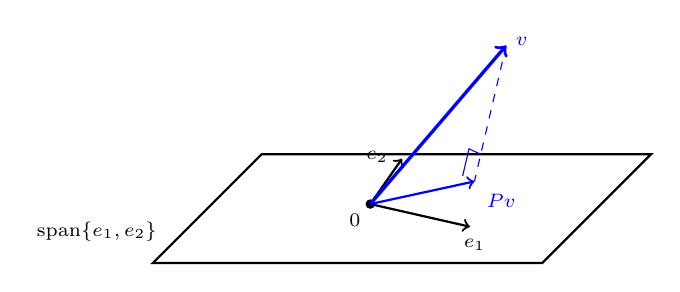
\begin{tikzpicture}[scale=1.15]
	% the plane spanned by e1, e2
	\draw[thick] (-2.4,-0.65) -- (1.9,-0.65) -- (3.1,0.55) -- (-1.2,0.55) -- cycle;
	\node[left] at (-2.25,-0.3) {\scriptsize $\spn\{e_1,e_2\}$};
	% origin
	\fill (0,0) circle (1.5pt);
	\node[below left] at (0,0) {\scriptsize $0$};
	% basis vectors
	\draw[->, thick] (0,0) -- (1.1,-0.25);
	\node[below] at (1.15,-0.28) {\scriptsize $e_1$};
	\draw[->, thick] (0,0) -- (0.35,0.5);
	\node[left] at (0.3,0.52) {\scriptsize $e_2$};
	% v and its projection
	\draw[->, very thick, color=blue] (0,0) -- (1.5,1.75);
	\node[color=blue, right] at (1.5,1.8) {\scriptsize $v$};
	\draw[->, thick, color=blue] (0,0) -- (1.15,0.25);
	\node[color=blue, below right] at (1.18,0.22) {\scriptsize $Pv$};
	\draw[dashed, color=blue] (1.5,1.75) -- (1.15,0.25);
	% right angle mark
	\draw[color=blue] (1.02,0.31) -- (1.09,0.61) -- (1.22,0.55);
\end{tikzpicture}
\end{center}

Now the fundamental construction. In a general normed space, a closed convex set need not contain a point closest to a given point; in a Hilbert space it always does, and uniquely.

\begin{theorem}[Projection onto a closed convex set]
	Let $H$ be a Hilbert space and $C \subseteq H$ a non-empty closed convex set. Then for every $v \in H$ there is a unique $P_Cv \in C$ with
	$$\norm{v - P_Cv} = \dist(v, C) = \inf_{c \in C}\norm{v - c}.$$
	Moreover $P_C v$ is characterised among points of $C$ by
	$$\re \ip{c - P_Cv}{v - P_Cv} \leq 0 \qquad \text{for all } c \in C,$$
	and $P_C$ is $1$-Lipschitz.
\end{theorem}

\begin{proof}
	\emph{Existence.} Let $d = \dist(v,C)$ and pick $c_n \in C$ with $\norm{v - c_n}\to d$. Apply the parallelogram law to $v - c_n$ and $v - c_m$:
	$$\norm{c_m - c_n}^2 = 2\norm{v-c_n}^2 + 2\norm{v-c_m}^2 - 4\left\|v - \tfrac{c_n+c_m}{2}\right\|^2.$$
	By convexity $\frac{c_n+c_m}{2} \in C$, so the last term is at least $4d^2$, giving
	$$\norm{c_m-c_n}^2 \leq 2\norm{v-c_n}^2 + 2\norm{v-c_m}^2 - 4d^2 \longrightarrow 0.$$
	So $(c_n)$ is Cauchy; by completeness it converges to some $c \in C$ ($C$ is closed), and $\norm{v-c}=d$.

	\emph{Uniqueness.} If $c, c'$ both realise the distance, the same computation gives $\norm{c-c'}^2 \leq 2d^2+2d^2-4d^2 = 0$.

	\emph{Variational characterisation.} Write $u = P_Cv$. For $c \in C$ and $t \in (0,1]$, convexity gives $u + t(c-u) \in C$, so
	$$\norm{v-u}^2 \leq \norm{v - u - t(c-u)}^2 = \norm{v-u}^2 - 2t\re\ip{c-u}{v-u} + t^2\norm{c-u}^2.$$
	Hence $2\re\ip{c-u}{v-u} \leq t\norm{c-u}^2$ for all $t \in (0,1]$; letting $t \to 0$ gives $\re\ip{c-u}{v-u}\leq0$. Conversely, if $u \in C$ satisfies this then for any $c \in C$,
	$$\norm{v-c}^2 = \norm{(v-u)-(c-u)}^2 = \norm{v-u}^2 - 2\re\ip{c-u}{v-u}+\norm{c-u}^2 \geq \norm{v-u}^2,$$
	so $u$ minimises.

	\emph{Lipschitz.} Let $u = P_Cv$, $u' = P_Cv'$. Adding the variational inequalities with $c = u'$ and $c = u$ respectively gives
	$$\re\ip{u'-u}{v-u} \leq 0, \qquad \re\ip{u-u'}{v'-u'}\leq 0,$$
	and adding, $\re\ip{u'-u}{(v-v')-(u-u')}\leq0$, i.e.\ $\norm{u-u'}^2 \leq \re\ip{u-u'}{v-v'}\leq \norm{u-u'}\norm{v-v'}$.
\end{proof}

The variational condition says that the vector from the closest point to $v$ makes an obtuse (or right) angle with every direction into $C$. If you draw it, the reason is obvious: if the angle were acute, we could move a little way into $C$ and get closer.

\begin{center}
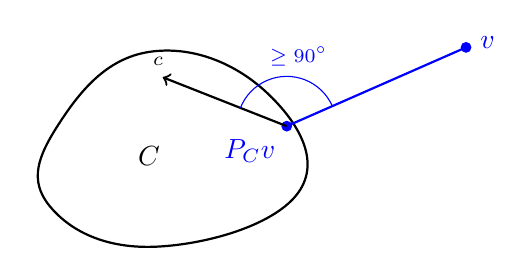
\begin{tikzpicture}[scale=1.15]
	% convex set
	\draw[thick] plot[smooth cycle, tension=0.75] coordinates {(-2.5,0.2) (-1.5,1.0) (-0.2,0.55) (0.15,-0.55) (-1.4,-1.15) (-2.6,-0.7)};
	\node at (-1.5,-0.15) {$C$};
	% external point
	\fill[color=blue] (2.0,1.05) circle (1.7pt);
	\node[color=blue, right] at (2.05,1.1) {$v$};
	% closest point
	\fill[color=blue] (0.02,0.18) circle (1.7pt);
	\node[color=blue, below left] at (0.0,0.14) {$P_Cv$};
	% segment
	\draw[thick, color=blue] (0.02,0.18) -- (2.0,1.05);
	% direction into C
	\draw[->, thick] (0.02,0.18) -- (-1.35,0.72);
	\node[above] at (-1.4,0.74) {\scriptsize $c$};
	% angle mark
	\draw[color=blue] (0.02,0.18) ++(23.7:0.55) arc (23.7:158.5:0.55);
	\node[color=blue] at (0.15,0.95) {\scriptsize $\geq 90^\circ$};
\end{tikzpicture}
\end{center}

Applying this to a closed subspace gives the decomposition that makes Hilbert space theory work.

\begin{theorem}[Orthogonal decomposition]
	Let $H$ be a Hilbert space and $M \subseteq H$ a closed subspace. Then
	$$H = M \oplus M^\perp,$$
	and the projection $P_M$ onto $M$ is linear, bounded with $\norm{P_M}\leq 1$, satisfies $P_M^2 = P_M$, and has $\ker P_M = M^\perp$, $\image P_M = M$. Moreover $(M^\perp)^\perp = M$.
\end{theorem}

\begin{proof}
	A subspace is convex and, being closed, the projection theorem applies. Let $v \in H$ and $u = P_M v$. The variational inequality reads $\re \ip{m - u}{v-u}\leq 0$ for all $m \in M$; as $M$ is a subspace, $m - u$ ranges over all of $M$, and replacing $m-u$ by $\lambda(m-u)$ for arbitrary $\lambda \in \F$ we conclude
	$$\ip{m}{v - u} = 0 \quad \text{for all } m \in M,$$
	i.e.\ $v - u \in M^\perp$. Hence $v = u + (v-u) \in M + M^\perp$. The sum is direct since $M \cap M^\perp = \{0\}$ (a vector orthogonal to itself is zero).

	Uniqueness of the decomposition gives linearity of $P_M$, and Pythagoras gives $\norm{v}^2 = \norm{P_Mv}^2 + \norm{v - P_Mv}^2 \geq \norm{P_M v}^2$, so $\norm{P_M}\leq 1$ (with equality unless $M = \{0\}$). Clearly $P_M^2 = P_M$, $\image P_M = M$ and $\ker P_M = M^\perp$.

	Finally $M \subseteq (M^\perp)^\perp$ is clear. Conversely if $v \in (M^\perp)^\perp$, write $v = u + w$ with $u \in M$, $w \in M^\perp$; then $w = v - u \in (M^\perp)^\perp$ too, and $w \in M^\perp \cap (M^\perp)^\perp = \{0\}$, so $v = u \in M$.
\end{proof}

\begin{center}
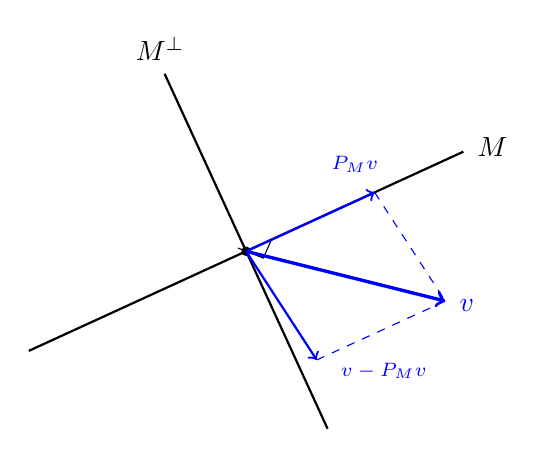
\begin{tikzpicture}[scale=1.15]
	% M as a slanted line
	\draw[thick] (-2.4,-1.1) -- (2.4,1.1);
	\node[right] at (2.45,1.15) {$M$};
	% M perp
	\draw[thick] (-0.9,1.96) -- (0.9,-1.96);
	\node[above] at (-0.95,2.0) {$M^\perp$};
	% right angle at origin
	\draw (0.28,0.128) -- (0.19,-0.075) -- (-0.09,0.036);
	\fill (0,0) circle (1.5pt);
	% vector v
	\draw[->, very thick, color=blue] (0,0) -- (2.2,-0.55);
	\node[color=blue, right] at (2.25,-0.6) {$v$};
	% components
	\draw[->, thick, color=blue] (0,0) -- (1.42,0.65);
	\node[color=blue, above] at (1.2,0.76) {\scriptsize $P_Mv$};
	\draw[->, thick, color=blue] (0,0) -- (0.78,-1.2);
	\node[color=blue, right] at (0.94,-1.32) {\scriptsize $v - P_Mv$};
	\draw[dashed, color=blue] (1.42,0.65) -- (2.2,-0.55);
	\draw[dashed, color=blue] (0.78,-1.2) -- (2.2,-0.55);
\end{tikzpicture}
\end{center}

\begin{corollary}
	Let $M \subseteq H$ be a subspace of a Hilbert space. Then $M$ is dense if and only if $M^\perp = \{0\}$.
\end{corollary}

\begin{proof}
	Apply the theorem to $\bar M$: we have $\bar M = (\bar M^\perp)^\perp = (M^\perp)^\perp$, which is $H$ exactly when $M^\perp = \{0\}$.
\end{proof}

\subsection{The Riesz Representation Theorem}

We can now compute the dual of a Hilbert space completely, and the answer is as beautiful as could be hoped: a Hilbert space is its own dual.

\begin{theorem}[Riesz--Fréchet Representation Theorem]
	Let $H$ be a Hilbert space and $f \in H^*$. Then there is a unique $w \in H$ with
	$$f(v) = \ip{v}{w} \qquad \text{for all } v \in H,$$
	and $\norm{f} = \norm{w}$. The map $w \mapsto \ip{\cdot}{w}$ is a conjugate-linear isometric bijection $H \to H^*$.
\end{theorem}

\begin{proof}
	\emph{Uniqueness.} If $\ip{v}{w} = \ip{v}{w'}$ for all $v$ then $w - w' \perp H$, so $w = w'$.

	\emph{Existence.} If $f = 0$ take $w = 0$. Otherwise $M = \ker f$ is a proper closed subspace, so by orthogonal decomposition $M^\perp \neq \{0\}$; pick $u \in M^\perp$ with $\norm{u}=1$, and note $f(u)\neq 0$ (else $u \in M \cap M^\perp$).

	For any $v \in H$, the vector
	$$v - \frac{f(v)}{f(u)}u$$
	lies in $\ker f = M$, hence is orthogonal to $u$. Taking the inner product with $u$ gives
	$$\ip{v}{u} - \frac{f(v)}{f(u)} = 0, \qquad \text{i.e.}\qquad f(v) = f(u)\ip{v}{u} = \ip{v}{\overline{f(u)}u}.$$
	So $w = \overline{f(u)}u$ works.

	\emph{Isometry.} $|f(v)| = |\ip{v}{w}| \leq \norm{v}\norm{w}$ by Cauchy--Schwarz, so $\norm{f}\leq\norm{w}$; and $f(w) = \norm{w}^2$ gives $\norm{f}\geq\norm{w}$. Conjugate-linearity of $w \mapsto \ip{\cdot}{w}$ is immediate.
\end{proof}

\begin{corollary}
	Every Hilbert space is reflexive.
\end{corollary}

\begin{proof}
	Write $\Phi : H \to H^*$ for the conjugate-linear bijection above. Then $H^*$ is itself a Hilbert space with $\ip{\Phi v}{\Phi w}_{H^*} = \ip{w}{v}_H$ (one checks the axioms; conjugating swaps the slots). Applying Riesz again gives a conjugate-linear bijection $\Psi : H^* \to H^{**}$, and $\Psi\circ\Phi : H \to H^{**}$ is a linear isometric bijection. A short computation shows $\Psi \circ \Phi = \iota$, the canonical embedding: for $v \in H$ and $f = \Phi w \in H^*$,
	$$(\Psi\Phi v)(f) = \ip{f}{\Phi v}_{H^*} = \ip{v}{w}_H = f(v) = \iota(v)(f).$$
	So $\iota$ is surjective.
\end{proof}

\subsection{Orthonormal Bases}

We now build coordinates. In a Hilbert space we want to allow infinite linear combinations, which changes the notion of `basis' completely from the Hamel bases of the previous sections.

\begin{proposition}[Gram--Schmidt]
	Let $(v_n)_{n \geq 1}$ be a linearly independent sequence in an inner product space. Then there is an orthonormal sequence $(e_n)$ with $\spn\{e_1,\dots,e_n\} = \spn\{v_1,\dots,v_n\}$ for every $n$.
\end{proposition}

\begin{proof}
	Inductively set $e_1 = v_1/\norm{v_1}$ and
	$$u_n = v_n - \sum_{i=1}^{n-1}\ip{v_n}{e_i}e_i, \qquad e_n = \frac{u_n}{\norm{u_n}}.$$
	Then $u_n \neq 0$ by linear independence, $u_n \perp e_i$ for $i<n$ by the computation in Pythagoras' theorem, and the spans agree by construction.
\end{proof}

\begin{example}[Legendre polynomials]
	Take $H = L^2[-1,1]$ with $\ip{f}{g}=\int_{-1}^1 f\bar g\dd x$, and apply Gram--Schmidt to the monomials $1, x, x^2, \dots$, which are linearly independent. We get $e_0 = 1/\sqrt2$, and then
	$$u_1 = x - \ip{x}{e_0}e_0 = x, \qquad e_1 = \sqrt{\tfrac32}\,x,$$
	since $\int_{-1}^1 x \dd x = 0$ and $\int_{-1}^1x^2\dd x = \frac23$. Next,
	$$u_2 = x^2 - \ip{x^2}{e_0}e_0 - \ip{x^2}{e_1}e_1 = x^2 - \tfrac13,$$
	using $\int_{-1}^1x^2\dd x = \frac23$ and $\int_{-1}^1 x^3\dd x = 0$; normalising, $e_2 = \sqrt{\frac{45}{8}}(x^2-\frac13)$.

	Up to normalisation these are the \vocab{Legendre polynomials} $P_n$ of IB Methods, with the standard normalisation $P_n(1)=1$ giving $P_0=1$, $P_1=x$, $P_2 = \frac12(3x^2-1)$ and $e_n = \sqrt{\frac{2n+1}{2}}P_n$. That they form an orthonormal \emph{basis} of $L^2[-1,1]$ follows from Stone--Weierstrass: the polynomials are dense in $C[-1,1]$ for the sup norm, hence in $L^2$, and their closed span is the closed span of the $e_n$.

	So the Legendre expansion of a function -- which in Methods appeared as a somewhat mysterious consequence of Sturm--Liouville theory -- is just the expansion in an orthonormal basis, and Parseval gives
	$$\int_{-1}^1|f|^2\dd x = \sum_{n\geq0}\frac{2n+1}{2}\left|\int_{-1}^1 f P_n \dd x\right|^2.$$
\end{example}

\begin{definition}[Orthonormal basis]
	An orthonormal family $(e_i)_{i \in I}$ in a Hilbert space $H$ is an \vocab{orthonormal basis} (or \vocab{complete orthonormal system}, or \vocab{Hilbert basis}) if $\overline{\spn\{e_i\}} = H$.
\end{definition}

\begin{proposition}
	For an orthonormal family $(e_i)_{i\in I}$ in a Hilbert space $H$, the following are equivalent:
	\begin{enumerate}[label=(\roman*)]
		\item $(e_i)$ is an orthonormal basis;
		\item $(e_i)$ is maximal among orthonormal families;
		\item $\{e_i\}^\perp = \{0\}$;
		\item $v = \sum_{i \in I}\ip{v}{e_i}e_i$ for every $v \in H$;
		\item (\emph{Parseval}) $\norm{v}^2 = \sum_{i \in I}|\ip{v}{e_i}|^2$ for every $v \in H$.
	\end{enumerate}
\end{proposition}

\begin{proof}
	(i) $\iff$ (iii) is the density criterion proved above. (ii) $\iff$ (iii): a unit vector orthogonal to all $e_i$ would enlarge the family, and conversely.

	(i) $\Rightarrow$ (iv). By Bessel, only countably many coefficients are non-zero, so list them as $i_1, i_2, \dots$ and set $s_n = \sum_{k \leq n}\ip{v}{e_{i_k}}e_{i_k}$. For $m<n$, Pythagoras gives $\norm{s_n - s_m}^2 = \sum_{m<k\leq n}|\ip{v}{e_{i_k}}|^2$, which tends to $0$ by Bessel; so $(s_n)$ is Cauchy and converges to some $s \in H$. Now $v - s$ is orthogonal to every $e_i$ (for $i = i_k$ this is a limit of the finite computation, and for other $i$ the coefficient is zero), so $v = s$ by (iii). The value of the sum does not depend on the ordering, since any rearrangement converges to a vector with the same inner products against all $e_i$.

	(iv) $\Rightarrow$ (v) is Pythagoras applied to the partial sums and passing to the limit, and (v) $\Rightarrow$ (iii) is immediate: if $v \perp$ all $e_i$ then $\norm{v}=0$.

	(iv) $\Rightarrow$ (i) is clear.
\end{proof}

\begin{proposition}
	Every Hilbert space has an orthonormal basis, and $H$ is separable if and only if it has a countable orthonormal basis.
\end{proposition}

\begin{proof}
	Existence: Zorn's lemma applied to the set of orthonormal families ordered by inclusion; the union of a chain of orthonormal families is orthonormal, and a maximal element is an orthonormal basis by (ii) above.

	If $H$ is separable with dense countable set $\{v_n\}$, discard those $v_n$ lying in the span of the earlier ones and apply Gram--Schmidt; the resulting orthonormal sequence has the same closed span, namely $H$. Conversely, given a countable orthonormal basis, the rational (or rational-complex) linear combinations of the $e_n$ form a countable dense set.
\end{proof}

\begin{theorem}[Classification of separable Hilbert spaces]
	Every infinite-dimensional separable Hilbert space is isometrically isomorphic to $\ell^2$.
\end{theorem}

\begin{proof}
	Let $(e_n)_{n\geq1}$ be a countable orthonormal basis of $H$ and define
	$$U : H \to \ell^2, \qquad Uv = \big(\ip{v}{e_n}\big)_{n\geq1}.$$
	By Bessel this lands in $\ell^2$, and by Parseval $\norm{Uv}_2 = \norm{v}$, so $U$ is a linear isometry, in particular injective.

	For surjectivity, let $a = (a_n)\in\ell^2$. The partial sums $s_N = \sum_{n\leq N}a_ne_n$ satisfy $\norm{s_N-s_M}^2 = \sum_{M<n\leq N}|a_n|^2 \to 0$, so by completeness of $H$ they converge to some $v$, and $\ip{v}{e_n} = a_n$ by continuity of the inner product. So $Uv = a$.
\end{proof}

This is a striking statement: up to isometric isomorphism there is only \emph{one} infinite-dimensional separable Hilbert space. Compare the situation for Banach spaces, where the spaces $\ell^1$, $\ell^2$, $c_0$, $C[0,1]$ and $L^1[0,1]$ are all separable and pairwise non-isomorphic. Hilbert space is a very rigid object.

\begin{example}[Fourier series]
	Take $H = L^2(\mathbb{T})$, the completion of $C(\mathbb{T})$ under $\ip{f}{g}=\frac{1}{2\pi}\int_{-\pi}^\pi f\bar g$. The family $e_k(x) = e^{ikx}$, $k \in \Z$, is orthonormal:
	$$\ip{e_k}{e_l} = \frac{1}{2\pi}\int_{-\pi}^{\pi}e^{i(k-l)x}\dd x = \delta_{kl}.$$
	It is an orthonormal basis: by Stone--Weierstrass the trigonometric polynomials are dense in $C(\mathbb{T})$ for the sup norm, hence for the $L^2$ norm (as $\norm{\cdot}_{L^2}\leq\norm{\cdot}_\infty$ here), and $C(\mathbb{T})$ is dense in $L^2(\mathbb{T})$ by construction.

	So for every $f \in L^2(\mathbb{T})$ the Fourier series converges in $L^2$,
	$$\left\| f - \sum_{|k|\leq N} \hat f(k)e_k \right\|_{L^2} \longrightarrow 0,$$
	and Parseval reads
	$$\frac{1}{2\pi}\int_{-\pi}^\pi |f|^2 \dd x = \sum_{k \in \Z}|\hat f(k)|^2.$$
	This is the theorem that was quoted without proof in IB Methods, and here it is at last, as a special case of a general principle: $L^2(\mathbb{T}) \cong \ell^2(\Z)$ via the Fourier coefficients.
\end{example}

\subsection{Adjoints on Hilbert Space}

Riesz representation lets us define an adjoint that lives on $H$ itself rather than on $H^*$, and this is the version that generalises the conjugate transpose from IB Linear Algebra.

\begin{proposition}
	Let $H$ be a Hilbert space and $T \in \Bop(H)$. Then there is a unique $T^* \in \Bop(H)$ with
	$$\ip{Tv}{w} = \ip{v}{T^*w} \qquad \text{for all } v,w \in H,$$
	and $\norm{T^*}=\norm{T}$.
\end{proposition}

\begin{proof}
	Fix $w$. The map $v \mapsto \ip{Tv}{w}$ is a bounded linear functional of norm at most $\norm{T}\norm{w}$, so by Riesz there is a unique vector, call it $T^*w$, with $\ip{Tv}{w}=\ip{v}{T^*w}$ for all $v$. Uniqueness of the Riesz vector makes $T^*$ well defined, and gives linearity: $T^*(\lambda w_1+w_2)$ and $\lambda T^*w_1 + T^*w_2$ represent the same functional. Also $\norm{T^*w}\leq\norm{T}\norm{w}$, so $\norm{T^*}\leq\norm{T}$; applying the same to $T^*$ and noting $T^{**}=T$ gives equality.
\end{proof}

\begin{proposition}
	For $S,T\in\Bop(H)$ and $\lambda \in \F$:
	\begin{enumerate}[label=(\roman*)]
		\item $(S+T)^*=S^*+T^*$, $(\lambda T)^* = \bar\lambda T^*$, $(ST)^*=T^*S^*$, $T^{**}=T$;
		\item $\norm{T^*T} = \norm{T}^2$;
		\item $\ker T = (\image T^*)^\perp$ and $\overline{\image T} = (\ker T^*)^\perp$.
	\end{enumerate}
\end{proposition}

\begin{proof}
	(i) All are routine verifications from the defining identity.

	(ii) $\norm{T^*T}\leq\norm{T^*}\norm{T}=\norm{T}^2$, and conversely
	$$\norm{Tv}^2 = \ip{Tv}{Tv} = \ip{T^*Tv}{v}\leq\norm{T^*T}\norm{v}^2,$$
	so $\norm{T}^2\leq\norm{T^*T}$. (This identity is the $C^*$-identity, and it is the reason $\Bop(H)$ is such a rigid algebra.)

	(iii) $v \in \ker T$ iff $Tv = 0$ iff $\ip{Tv}{w}=0$ for all $w$ iff $\ip{v}{T^*w}=0$ for all $w$ iff $v \perp \image T^*$. Taking orthogonal complements and using $(M^\perp)^\perp = \bar M$ for a subspace gives the second identity applied to $T^*$.
\end{proof}

\begin{definition}
	Let $T \in \Bop(H)$. We say $T$ is
	\begin{enumerate}[label=(\roman*)]
		\item \vocab{self-adjoint} (or Hermitian) if $T = T^*$;
		\item \vocab{unitary} if $T^*T = TT^* = I$;
		\item \vocab{normal} if $T^*T = TT^*$.
	\end{enumerate}
\end{definition}

Self-adjoint and unitary operators are normal. Unitaries are exactly the surjective isometries of $H$: $\norm{Uv}^2 = \ip{U^*Uv}{v}=\norm{v}^2$.

\begin{example}
	\begin{enumerate}[label=(\roman*)]
		\item On $\F^n$, the adjoint of a matrix $A$ is the conjugate transpose $\bar A^{\mathsf T}$, and self-adjoint means Hermitian.
		\item On $\ell^2$, the left and right shifts satisfy $L = R^*$: indeed $\ip{Rx}{y} = \sum_{n\geq2}x_{n-1}\bar y_n = \sum_{n\geq1}x_n \bar y_{n+1}=\ip{x}{Ly}$. Neither is normal.
		\item The diagonal operator $M_\lambda$ on $\ell^2$ has $M_\lambda^* = M_{\bar\lambda}$, so it is normal, and self-adjoint exactly when all $\lambda_n$ are real.
		\item The integral operator on $L^2[0,1]$ with kernel $k$ has adjoint the integral operator with kernel $k^*(x,y)=\overline{k(y,x)}$. It is self-adjoint when $k$ is Hermitian, $k(y,x)=\overline{k(x,y)}$; this is the Hilbert space form of the symmetric Sturm--Liouville kernels from IB Methods.
	\end{enumerate}
\end{example}

\begin{proposition}
	Let $T \in \Bop(H)$ with $H$ complex.
	\begin{enumerate}[label=(\roman*)]
		\item $T$ is self-adjoint if and only if $\ip{Tv}{v}\in\R$ for all $v$.
		\item If $T$ is self-adjoint then $\norm{T} = \sup_{\norm{v}\leq1}|\ip{Tv}{v}|$.
		\item If $T$ is normal then $\ker T = \ker T^*$, and eigenvectors for distinct eigenvalues are orthogonal.
	\end{enumerate}
\end{proposition}

\begin{proof}
	(i) If $T = T^*$ then $\ip{Tv}{v}=\ip{v}{Tv}=\overline{\ip{Tv}{v}}$. Conversely, suppose $\ip{Tv}{v}\in\R$ for all $v$. Then $\ip{(T-T^*)v}{v}=0$ for all $v$, and over $\C$ this forces $T = T^*$: expanding $\ip{S(v+w)}{v+w}=0$ and $\ip{S(v+iw)}{v+iw}=0$ for $S = T-T^*$ gives $\ip{Sv}{w}=0$ for all $v,w$.

	(ii) Write $M$ for the supremum. Clearly $M \leq \norm{T}$. For the converse, note that for self-adjoint $T$,
	$$\ip{T(v+w)}{v+w}-\ip{T(v-w)}{v-w} = 4\re\ip{Tv}{w}.$$
	The left-hand side is at most $M(\norm{v+w}^2+\norm{v-w}^2)=2M(\norm{v}^2+\norm{w}^2)$ in absolute value. Taking $\norm{v}=\norm{w}=1$ gives $\re\ip{Tv}{w}\leq M$, and choosing a phase, $|\ip{Tv}{w}|\leq M$; taking $w = Tv/\norm{Tv}$ gives $\norm{Tv}\leq M$.

	(iii) If $T$ is normal then $\norm{Tv}^2 = \ip{T^*Tv}{v} = \ip{TT^*v}{v} = \norm{T^*v}^2$, so the kernels agree. If $Tv=\lambda v$ and $Tw=\mu w$ with $\lambda \neq \mu$, note $T - \lambda I$ is normal so $T^*v = \bar\lambda v$, and then
	$$\lambda\ip{v}{w} = \ip{Tv}{w}=\ip{v}{T^*w}=\ip{v}{\bar\mu w}=\mu\ip{v}{w},$$
	forcing $\ip{v}{w}=0$.
\end{proof}

\section{Spectral Theory}

In IB Linear Algebra, the key to understanding a linear map on a finite-dimensional space was its eigenvalues. In infinite dimensions eigenvalues are not enough -- an operator can fail to be invertible without having any eigenvalues at all -- and the right generalisation is the \emph{spectrum}.

Throughout this section $X$ is a complex Banach space (complex is essential: over $\R$ even a rotation of the plane has empty spectrum) and $T \in \Bop(X)$. We abbreviate $T - \lambda I$ to $T - \lambda$.

\subsection{The Spectrum and the Resolvent}

\begin{definition}[Spectrum and resolvent]
	Let $T \in \Bop(X)$. The \vocab{resolvent set} of $T$ is
	$$\rho(T) = \{ \lambda \in \C : T - \lambda \ \text{is a bijection } X\to X \},$$
	and the \vocab{spectrum} is $\sigma(T) = \C \setminus \rho(T)$. For $\lambda \in \rho(T)$ the \vocab{resolvent} is
	$$R_\lambda = R_T(\lambda) = (T-\lambda)^{-1} \in \Bop(X).$$
\end{definition}

Two remarks on the definition. First, we only demanded that $T - \lambda$ be a bijection; by the inverse mapping theorem the inverse is then automatically bounded, so we get $R_\lambda \in \Bop(X)$ for free. This is a nice payoff from the Baire category theorem. Second, $\lambda$ is an eigenvalue exactly when $T - \lambda$ fails to be \emph{injective}; but it can also fail to be \emph{surjective}, and that also puts $\lambda$ in the spectrum. So eigenvalues form only part of the spectrum.

\begin{definition}[Parts of the spectrum]
	Let $\lambda\in\sigma(T)$. We say $\lambda$ lies in
	\begin{enumerate}[label=(\roman*)]
		\item the \vocab{point spectrum} $\sigma_p(T)$ if $T-\lambda$ is not injective; the elements of $\ker(T-\lambda)\setminus\{0\}$ are \vocab{eigenvectors} and $\lambda$ an \vocab{eigenvalue};
		\item the \vocab{continuous spectrum} $\sigma_c(T)$ if $T-\lambda$ is injective with dense but proper range;
		\item the \vocab{residual spectrum} $\sigma_r(T)$ if $T-\lambda$ is injective with non-dense range.
	\end{enumerate}
	We also define the \vocab{approximate point spectrum}
	$$\sigma_{\mathrm{ap}}(T) = \{ \lambda : \exists\, v_n \text{ with } \norm{v_n}=1 \text{ and } \norm{(T-\lambda)v_n}\to0 \}.$$
\end{definition}

These three parts are disjoint and cover $\sigma(T)$. Note $\sigma_p \subseteq \sigma_{\mathrm{ap}}$, and $\lambda \in \sigma_{\mathrm{ap}}$ exactly when $T - \lambda$ is not bounded below.

\begin{theorem}
	Let $T \in \Bop(X)$ with $X$ a complex Banach space. Then:
	\begin{enumerate}[label=(\roman*)]
		\item $\rho(T)$ is open and $\lambda\mapsto R_\lambda$ is analytic on it;
		\item $\sigma(T)\subseteq\{\lambda : |\lambda|\leq\norm{T}\}$, so $\sigma(T)$ is compact;
		\item $\sigma(T)\neq\emptyset$.
	\end{enumerate}
\end{theorem}

\begin{proof}
	(ii) If $|\lambda|>\norm{T}$ then $\norm{T/\lambda}<1$, so by the Neumann series $I - T/\lambda$ is invertible, hence so is $T - \lambda = -\lambda(I - T/\lambda)$. Moreover
	\begin{equation*}
		R_\lambda = -\frac{1}{\lambda}\sum_{n=0}^\infty \left(\frac{T}{\lambda}\right)^n, \qquad \norm{R_\lambda}\leq\frac{1}{|\lambda|-\norm{T}}. \tag{$*$}
	\end{equation*}
	So $\sigma(T)$ is contained in the closed disc of radius $\norm{T}$, and it is closed by (i).

	(i) Let $\lambda_0\in\rho(T)$. For $\lambda$ near $\lambda_0$ write
	$$T - \lambda = (T-\lambda_0) - (\lambda - \lambda_0) = (T-\lambda_0)\big( I - (\lambda-\lambda_0)R_{\lambda_0}\big).$$
	If $|\lambda - \lambda_0| < \norm{R_{\lambda_0}}^{-1}$ the bracket is invertible by the Neumann series, so $\lambda \in\rho(T)$ and
	$$R_\lambda = \left( \sum_{n=0}^\infty (\lambda-\lambda_0)^n R_{\lambda_0}^n \right) R_{\lambda_0} = \sum_{n=0}^\infty R_{\lambda_0}^{n+1}(\lambda-\lambda_0)^n.$$
	Thus $\rho(T)$ is open and $R_\lambda$ is given locally by a convergent power series in $\lambda$ with coefficients in $\Bop(X)$: it is analytic, with $\frac{\dd}{\dd\lambda}R_\lambda = R_\lambda^2$.

	(iii) Suppose for contradiction $\sigma(T)=\emptyset$, so $R_\lambda$ is defined and analytic on all of $\C$. Fix $\varphi \in \Bop(X)^*$ and let $g(\lambda) = \varphi(R_\lambda)$. Composing an analytic $\Bop(X)$-valued function with a bounded functional gives an analytic function $\C\to\C$, so $g$ is entire. By $(*)$, $\norm{R_\lambda}\to0$ as $|\lambda|\to\infty$, hence $g(\lambda)\to0$; in particular $g$ is bounded. By Liouville's theorem from IB Complex Analysis, $g$ is constant, and the constant is $0$.

	This holds for every $\varphi \in \Bop(X)^*$, so by Hahn--Banach (which says the dual separates points) $R_\lambda = 0$ for every $\lambda$. But $R_\lambda$ is a bijection and $X \neq \{0\}$, so this is absurd.
\end{proof}

\begin{remark}
	The proof of (iii) is where complex scalars are indispensable. Over $\R$, the rotation by $90^\circ$ on $\R^2$ has $T-\lambda$ invertible for every real $\lambda$.
\end{remark}

\begin{center}
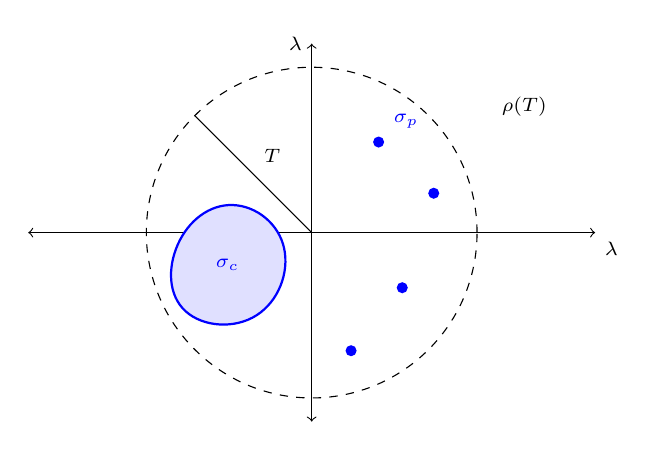
\begin{tikzpicture}[scale=1.0]
	% complex plane
	\draw[<->] (-3.6,0) -- (3.6,0);
	\draw[<->] (0,-2.4) -- (0,2.4);
	\node[below right] at (3.6,0) {\scriptsize $\re\lambda$};
	\node[left] at (0,2.4) {\scriptsize $\im\lambda$};
	% disc of radius ||T||
	\draw[dashed] (0,0) circle (2.1);
	\draw (0,0) -- (-1.485,1.485);
	\node at (-0.5,0.98) {\scriptsize $\norm{T}$};
	% spectrum: a blob (continuous spectrum) plus isolated eigenvalues
	\draw[thick, color=blue, fill=blue!12] plot[smooth cycle, tension=0.8] coordinates {(-1.7,-0.15) (-1.0,0.35) (-0.35,-0.2) (-0.7,-1.05) (-1.6,-1.0)};
	\node[color=blue] at (-1.07,-0.41) {\scriptsize $\sigma_c$};
	\foreach \p in {(0.85,1.15), (1.55,0.5), (1.15,-0.7), (0.5,-1.5)} {
		\fill[color=blue] \p circle (2pt);
	}
	\node[color=blue, above right] at (0.92,1.2) {\scriptsize $\sigma_p$};
	\node at (2.7,1.6) {\scriptsize $\rho(T)$};
\end{tikzpicture}
\end{center}

\begin{example}[Multiplication operators]
	Let $\lambda = (\lambda_n)\in\ell^\infty$ and $M_\lambda$ the diagonal operator on $\ell^2$. Then $M_\lambda - \mu$ is the diagonal operator with entries $\lambda_n - \mu$, which is invertible precisely when $\inf_n|\lambda_n-\mu|>0$. Hence
	$$\sigma(M_\lambda) = \overline{\{\lambda_n : n \in\N\}},$$
	with $\sigma_p = \{\lambda_n\}$ and the remaining limit points forming the continuous spectrum. In particular every non-empty compact subset of $\C$ arises as a spectrum: take $\{\lambda_n\}$ to be a countable dense subset of it.
\end{example}

\begin{example}[Shift operators]
	Consider $L, R$ on $\ell^2$, with $L = R^*$.

	For $R$: it is an isometry, so $\norm{Rx-\mu x}\geq(1-|\mu|)\norm{x}$ shows $R - \mu$ is bounded below for $|\mu|<1$; but its range is not dense, since $\image(R-\mu)^\perp = \ker(L - \bar\mu)$ and $L y = \bar\mu y$ is solved by $y = (1, \bar\mu, \bar\mu^2, \dots)\in\ell^2$. So $\{|\mu|<1\}\subseteq\sigma_r(R)$. Also $R$ has no eigenvalues: $Rx = \mu x$ forces $x = 0$ by comparing coordinates. Since $\sigma(R)$ is closed and contained in the closed unit disc, $\sigma(R) = \bar{D}$, with the open disc residual and the unit circle continuous spectrum.

	For $L$: for $|\mu|<1$ the vector $x = (1,\mu,\mu^2,\dots)$ lies in $\ell^2$ and satisfies $Lx = \mu x$. So the open disc is point spectrum, and again $\sigma(L)=\bar D$, with the circle as continuous spectrum.

	These are worth internalising. $R$ is injective but not surjective, $L$ is surjective but not injective, and their spectra are nonetheless the same closed disc.
\end{example}

\begin{proposition}
	Let $T \in \Bop(X)$. Then $\partial\sigma(T)\subseteq\sigma_{\mathrm{ap}}(T)$; in particular $\sigma_{\mathrm{ap}}(T)\neq\emptyset$.
\end{proposition}

\begin{proof}
	Let $\lambda\in\partial\sigma(T)$ and take $\lambda_n \in\rho(T)$ with $\lambda_n\to\lambda$. We claim $\norm{R_{\lambda_n}}\to\infty$. If not, pass to a subsequence with $\norm{R_{\lambda_n}}\leq M$; then for $n$ large, $|\lambda-\lambda_n|<M^{-1}$, and the Neumann series argument used to prove openness of $\rho(T)$ shows $\lambda\in\rho(T)$, a contradiction.

	So choose unit vectors $w_n$ with $\norm{R_{\lambda_n}w_n}\geq\frac12\norm{R_{\lambda_n}}$ and set $v_n = R_{\lambda_n}w_n/\norm{R_{\lambda_n}w_n}$. Then $\norm{v_n}=1$ and
	$$\norm{(T-\lambda_n)v_n} = \frac{\norm{w_n}}{\norm{R_{\lambda_n}w_n}}\leq\frac{2}{\norm{R_{\lambda_n}}}\longrightarrow0,$$
	so $\norm{(T-\lambda)v_n}\leq\norm{(T-\lambda_n)v_n}+|\lambda_n-\lambda|\to0$. Hence $\lambda\in\sigma_{\mathrm{ap}}(T)$. The last claim holds since $\sigma(T)$ is a non-empty compact set, so has non-empty boundary.
\end{proof}

\begin{remark}[Spectral radius]
	Define the \vocab{spectral radius} $r(T) = \sup_{\lambda\in\sigma(T)}|\lambda|$, which we have shown satisfies $r(T)\leq\norm{T}$. In fact Gelfand's formula holds:
	$$r(T) = \lim_{n\to\infty}\norm{T^n}^{1/n},$$
	the limit existing by subadditivity of $n \mapsto \log\norm{T^n}$. The proof runs by considering the Laurent expansion $R_\lambda = -\sum_{n\geq0}T^n\lambda^{-n-1}$, valid for $|\lambda|>\norm{T}$ and, by analyticity of the resolvent, for $|\lambda|>r(T)$; comparing radii of convergence gives the formula. For a self-adjoint operator on Hilbert space, $\norm{T^2}=\norm{T}^2$ by the $C^*$-identity, so $\norm{T^{2^k}}=\norm{T}^{2^k}$ and hence $r(T)=\norm{T}$ -- recovering a fact we proved by hand above.
\end{remark}

\begin{proposition}
	Let $T\in\Bop(X)$. Then $\sigma(T^*) = \sigma(T)$, where $T^*$ is the Banach space adjoint. If $H$ is a complex Hilbert space and $T\in\Bop(H)$, then $\sigma(T^*) = \overline{\sigma(T)}=\{\bar\lambda : \lambda\in\sigma(T)\}$.
\end{proposition}

\begin{proof}
	$T - \lambda$ is invertible if and only if $(T-\lambda)^* = T^*-\lambda$ is, since taking adjoints is multiplicative and $I^*=I$; and if $S$ is a two-sided inverse of $T-\lambda$ then $S^*$ is one for $T^*-\lambda$. Conversely if $T^*-\lambda$ is invertible then so is $T^{**}-\lambda$, and $T-\lambda$ is invertible by restricting to the image of the canonical embedding. On Hilbert space the adjoint is conjugate-linear in the scalar, whence the conjugation.
\end{proof}

\begin{proposition}
	Let $H$ be a complex Hilbert space and $T\in\Bop(H)$ self-adjoint. Then
	\begin{enumerate}[label=(\roman*)]
		\item $\sigma(T)\subseteq\R$;
		\item $\sigma_r(T)=\emptyset$;
		\item writing $m = \inf_{\norm{v}=1}\ip{Tv}{v}$ and $M = \sup_{\norm{v}=1}\ip{Tv}{v}$, we have $\sigma(T)\subseteq[m,M]$ and $m, M\in\sigma(T)$.
	\end{enumerate}
\end{proposition}

\begin{proof}
	(i) Let $\lambda = a+ib$ with $b \neq 0$. For any $v$,
	$$\norm{(T-\lambda)v}\norm{v}\geq|\ip{(T-\lambda)v}{v}|\geq|\im\ip{(T-\lambda)v}{v}| = |b|\norm{v}^2,$$
	using that $\ip{Tv}{v}$ is real. So $T-\lambda$ is bounded below, hence injective with closed range. The same estimate applies to $T - \bar\lambda = (T-\lambda)^*$, so $\ker(T-\lambda)^*=\{0\}$, and therefore $\overline{\image(T-\lambda)} = (\ker(T-\lambda)^*)^\perp = H$. A closed dense range is everything, so $T-\lambda$ is a bijection.

	(ii) If $T-\lambda$ has non-dense range then $\ker(T-\bar\lambda) = \ker(T-\lambda)^* \neq\{0\}$; by (i) $\lambda$ is real, so $\lambda$ is an eigenvalue and lies in $\sigma_p$, not $\sigma_r$.

	(iii) Let $\lambda>M$ be real and set $\delta = \lambda - M>0$. Then
	$$\ip{(\lambda - T)v}{v} = \lambda\norm{v}^2 - \ip{Tv}{v}\geq\delta\norm{v}^2,$$
	so $\norm{(T-\lambda)v}\geq\delta\norm{v}$ by Cauchy--Schwarz, and as in (i) we conclude $T-\lambda$ is invertible. Similarly for $\lambda<m$. For the last claim, suppose $M \in \rho(T)$; then $S = M - T$ is a positive self-adjoint operator ($\ip{Sv}{v}\geq0$) which is invertible and bounded below by some $\delta>0$. But $\inf_{\norm{v}=1}\ip{Sv}{v} = 0$ by definition of $M$, and for a positive operator the Cauchy--Schwarz inequality for the semi-inner product $(v,w)\mapsto\ip{Sv}{w}$ gives
	$$\norm{Sv}^2 = \ip{Sv}{Sv}\leq\ip{Sv}{v}^{1/2}\ip{S(Sv)}{Sv}^{1/2}\leq \ip{Sv}{v}^{1/2}\norm{S}^{3/2}\norm{v},$$
	so $\ip{Sv}{v}$ small forces $\norm{Sv}$ small -- contradicting boundedness below. Hence $M\in\sigma(T)$, and similarly $m$.
\end{proof}

\begin{corollary}
	If $T$ is self-adjoint then $\norm{T} = \max(|m|,|M|) = \sup_{\lambda\in\sigma(T)}|\lambda|$.
\end{corollary}

\begin{proof}
	We proved $\norm{T} = \sup_{\norm{v}\leq1}|\ip{Tv}{v}| = \max(|m|,|M|)$ earlier, and $m, M \in \sigma(T)\subseteq[m,M]$.
\end{proof}

\section{Compact Operators}

The failure of compactness of the unit ball was the first infinite-dimensional pathology we met. Compact operators are those that repair it: they are the operators which do send the unit ball into something with compact closure. They behave, in many respects, like matrices, and they have a genuinely satisfactory spectral theory.

\subsection{Definition and Examples}

\begin{definition}[Compact operator]
	Let $X, Y$ be normed spaces. A linear map $T : X \to Y$ is \vocab{compact} if $\overline{T(\bar B_X)}$ is compact in $Y$. We write $\Kop(X,Y)$ for the set of compact operators, and $\Kop(X)=\Kop(X,X)$.
\end{definition}

Equivalently (when $Y$ is complete, and using that compactness and sequential compactness agree in metric spaces), $T$ is compact if and only if every bounded sequence $(x_n)$ in $X$ has a subsequence with $(Tx_{n_k})$ convergent. A compact operator is automatically bounded, since a compact set is bounded.

\begin{center}
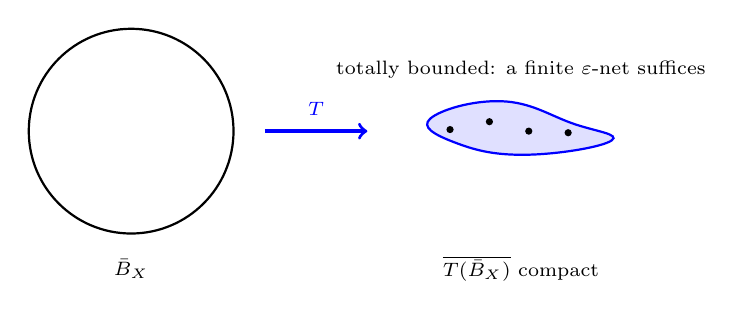
\begin{tikzpicture}[scale=1.0]
	% unit ball
	\draw[thick] (-3.2,0) circle (1.3);
	\node at (-3.2,-1.75) {\scriptsize $\bar B_X$};
	% arrow
	\draw[->, very thick, color=blue] (-1.5,0) -- (-0.2,0);
	\node[above, color=blue] at (-0.85,0.08) {\scriptsize $T$};
	% squashed image: a thin flattened blob
	\draw[thick, color=blue, fill=blue!12] plot[smooth cycle, tension=0.75] coordinates {(0.6,0.16) (1.5,0.38) (2.4,0.1) (2.9,-0.12) (1.8,-0.3) (0.9,-0.14)};
	\node at (1.75,-1.75) {\scriptsize $\overline{T(\bar B_X)}$ compact};
	% dashed finite net
	\foreach \p in {(0.85,0.02), (1.35,0.12), (1.85,0.0), (2.35,-0.02)} {
		\fill \p circle (1.3pt);
	}
	\node at (1.75,0.78) {\scriptsize totally bounded: a finite $\varepsilon$-net suffices};
\end{tikzpicture}
\end{center}

\begin{example}
	\begin{enumerate}[label=(\roman*)]
		\item Any bounded operator with finite-dimensional range is compact: $T(\bar B_X)$ is a bounded subset of a finite-dimensional space, whose closure is compact by Riesz. We call such $T$ a \vocab{finite rank} operator.
		\item The identity on $X$ is compact if and only if $\dim X<\infty$, by Riesz's theorem.
		\item The diagonal operator $M_\lambda$ on $\ell^2$ is compact if and only if $\lambda_n \to 0$. If $\lambda_n\to0$, then $M_\lambda$ is the operator-norm limit of the finite rank truncations $M_{\lambda^{(N)}}$, where $\lambda^{(N)}$ agrees with $\lambda$ up to $N$ and vanishes after; indeed $\norm{M_\lambda - M_{\lambda^{(N)}}} = \sup_{n>N}|\lambda_n|\to0$. Compactness then follows from the closedness theorem below. Conversely, if $|\lambda_{n_k}|\geq\delta>0$ then $(M_\lambda e_{n_k})$ has no convergent subsequence, as $\norm{M_\lambda e_{n_k}-M_\lambda e_{n_l}}\geq \delta\sqrt2$.
		\item The integral operator with continuous kernel $k$ on $C[0,1]$ is compact -- this is exactly what we proved with Arzelà--Ascoli. The same operator on $L^2[0,1]$ is compact too.
	\end{enumerate}
\end{example}

\begin{theorem}
	Let $X$ be a normed space and $Y$ a Banach space. Then $\Kop(X,Y)$ is a closed linear subspace of $\Bop(X,Y)$. Moreover $\Kop(X)$ is a two-sided ideal in $\Bop(X)$: if $T$ is compact and $S$ bounded, then $ST$ and $TS$ are compact.
\end{theorem}

\begin{proof}
	\emph{Subspace.} If $S,T$ are compact and $(x_n)$ is bounded, extract a subsequence along which $Sx_n$ converges, then a further subsequence along which $Tx_n$ converges; then $(S+\lambda T)x_n$ converges along it.

	\emph{Closed.} Let $T_n\in\Kop(X,Y)$ with $T_n\to T$ in operator norm. We show $T(\bar B_X)$ is totally bounded; since $Y$ is complete, this gives compact closure. Let $\varepsilon>0$ and choose $n$ with $\norm{T-T_n}<\varepsilon/2$. As $T_n(\bar B_X)$ is totally bounded, there are $y_1,\dots,y_m$ forming an $\varepsilon/2$-net for it. Then for $\norm{x}\leq1$ pick $j$ with $\norm{T_nx - y_j}<\varepsilon/2$, and
	$$\norm{Tx - y_j}\leq\norm{Tx-T_nx}+\norm{T_nx-y_j}<\varepsilon.$$
	So $\{y_j\}$ is an $\varepsilon$-net for $T(\bar B_X)$.

	\emph{Ideal.} If $T$ is compact and $S$ bounded: $ST(\bar B_X) \subseteq S(\overline{T(\bar B_X)})$, the continuous image of a compact set, hence has compact closure. And $TS(\bar B_X)\subseteq \norm{S}\, T(\bar B_X)$, which has compact closure.
\end{proof}

\begin{corollary}
	An operator-norm limit of finite rank operators is compact.
\end{corollary}

In a Hilbert space, the converse holds too, and this is a very useful way to think about compact operators.

\begin{theorem}[Finite rank approximation]
	Let $H$ be a Hilbert space and $T\in\Bop(H)$. Then $T$ is compact if and only if $T$ is the operator-norm limit of finite rank operators.
\end{theorem}

\begin{proof}
	($\Leftarrow$) is the corollary above.

	($\Rightarrow$) Let $T$ be compact and $\varepsilon>0$. By total boundedness there are $v_1,\dots,v_n$ with $T(\bar B_H)\subseteq\bigcup_j B(Tv_j,\varepsilon)$ -- we may take the net to consist of points of the image. Let $M = \spn\{Tv_1,\dots,Tv_n\}$, a finite-dimensional (hence closed) subspace, and let $P$ be the orthogonal projection onto $M$. Set $T_\varepsilon = PT$, which has finite rank.

	For $\norm{v}\leq1$, choose $j$ with $\norm{Tv - Tv_j}<\varepsilon$. Since $Tv_j \in M$ and $P$ is the nearest-point projection onto $M$,
	$$\norm{Tv - PTv} = \dist(Tv, M)\leq\norm{Tv - Tv_j}<\varepsilon.$$
	Hence $\norm{T - T_\varepsilon}\leq\varepsilon$.
\end{proof}

\begin{remark}
	This is false in general Banach spaces. Per Enflo constructed in 1973 a Banach space with a compact operator that is not a limit of finite rank operators -- resolving the `approximation problem' negatively, and famously earning him a live goose from Mazur.
\end{remark}

\begin{proposition}
	Let $H$ be a Hilbert space and $T \in \Bop(H)$. Then $T$ is compact if and only if $T^*$ is.
\end{proposition}

\begin{proof}
	If $T$ is compact, write $T = \lim T_n$ with $T_n$ finite rank. Then $T_n^*$ has finite rank (its range is contained in $\image T_n^{\,*}$, and $\rank T_n^* = \rank T_n$ since $\ker T_n^* = (\image T_n)^\perp$), and $\norm{T^*-T_n^*}=\norm{T-T_n}\to0$. So $T^*$ is compact. The converse follows as $T^{**}=T$.
\end{proof}

\begin{definition}[Hilbert--Schmidt operator]
	Let $H$ be a separable Hilbert space with orthonormal basis $(e_n)$. An operator $T \in \Bop(H)$ is \vocab{Hilbert--Schmidt} if
	$$\norm{T}_{\mathrm{HS}} = \left( \sum_n \norm{Te_n}^2 \right)^{1/2} < \infty.$$
\end{definition}

\begin{proposition}
	The quantity $\norm{T}_{\mathrm{HS}}$ is independent of the choice of orthonormal basis, $\norm{T}\leq\norm{T}_{\mathrm{HS}}$, and every Hilbert--Schmidt operator is compact.
\end{proposition}

\begin{proof}
	If $(f_m)$ is another orthonormal basis then by Parseval, applied twice,
	$$\sum_n \norm{Te_n}^2 = \sum_n\sum_m|\ip{Te_n}{f_m}|^2 = \sum_m\sum_n|\ip{e_n}{T^*f_m}|^2 = \sum_m\norm{T^*f_m}^2,$$
	and the right-hand side does not involve $(e_n)$; applying the same argument to $T^*$ shows it equals $\sum_m\norm{Tf_m}^2$. For the norm bound, write $v = \sum_n\ip{v}{e_n}e_n$ with $\norm{v}\leq1$; then by Cauchy--Schwarz $\norm{Tv}\leq\sum_n|\ip{v}{e_n}|\norm{Te_n}\leq\norm{v}\norm{T}_{\mathrm{HS}}$.

	For compactness, let $P_N$ be the projection onto $\spn\{e_1,\dots,e_N\}$. Then $TP_N$ has finite rank and $\norm{T - TP_N}\leq\norm{T-TP_N}_{\mathrm{HS}} = (\sum_{n>N}\norm{Te_n}^2)^{1/2}\to0$, so $T$ is a limit of finite rank operators.
\end{proof}

\begin{example}
	The diagonal operator $M_\lambda$ on $\ell^2$ is Hilbert--Schmidt exactly when $\lambda \in \ell^2$, compact exactly when $\lambda\in c_0$, and bounded exactly when $\lambda\in\ell^\infty$. So the Hilbert--Schmidt operators form a proper subclass of the compact operators; taking $\lambda_n = 1/\log(n+1)$ gives a compact operator that is not Hilbert--Schmidt. The integral operator on $L^2[0,1]$ with kernel $k \in L^2([0,1]^2)$ is always Hilbert--Schmidt, with $\norm{T}_{\mathrm{HS}}=\norm{k}_{L^2}$.
\end{example}

\subsection{Spectral Theory of Compact Operators}

Compact operators have spectra that look very much like those of matrices.

\begin{theorem}
	Let $X$ be a complex Banach space, $T\in\Kop(X)$ and $\lambda\neq0$. Then:
	\begin{enumerate}[label=(\roman*)]
		\item $\ker(T-\lambda)$ is finite-dimensional;
		\item $\image(T-\lambda)$ is closed;
		\item $T - \lambda$ is injective if and only if it is surjective.
	\end{enumerate}
	Consequently $\sigma(T)\setminus\{0\}$ consists of eigenvalues of finite multiplicity.
\end{theorem}

\begin{proof}
	(i) Let $N = \ker(T-\lambda)$. On $N$ we have $T = \lambda I$, so the restriction of $T$ to $N$ is $\lambda$ times the identity, which is compact (a restriction of a compact operator to a closed invariant subspace is compact). As $\lambda\neq0$, the identity on $N$ is compact, so $\dim N<\infty$ by Riesz.

	(ii) By (i), $N$ is finite-dimensional, hence complemented: $X = N\oplus Z$ for some closed subspace $Z$ (choose a basis $x_1,\dots,x_k$ of $N$, extend the coordinate functionals to $X^*$ by Hahn--Banach, and let $Z$ be the intersection of their kernels). Then $T - \lambda$ restricted to $Z$ is injective with the same range.

	We claim $S := (T-\lambda)|_Z$ is bounded below. If not, there are $z_n\in Z$ with $\norm{z_n}=1$ and $Sz_n\to0$. By compactness pass to a subsequence with $Tz_n \to y$. Then $\lambda z_n = Tz_n - Sz_n \to y$, so $z_n \to y/\lambda =: z \in Z$ with $\norm{z}=1$, and by continuity $Sz = 0$ -- contradicting injectivity on $Z$. So $S$ is bounded below, and a bounded-below operator has closed range: if $Sz_n \to w$ then $(z_n)$ is Cauchy, so $z_n\to z$ and $w = Sz$.

	(iii) Suppose $T-\lambda$ is injective but not surjective. Set $X_n = \image(T-\lambda)^n$. Each $X_n$ is closed (by (ii) and induction, since $(T-\lambda)^n = (-\lambda)^n + (\text{compact})$, using that $\Kop$ is an ideal), and
	$$X \supsetneq X_1\supsetneq X_2 \supsetneq\cdots,$$
	the inclusions being strict because $T-\lambda$ is injective (if $X_{n+1}=X_n$ then applying injectivity $n$ times gives $X_1 = X$).

	By Riesz's lemma choose $x_n\in X_n$ with $\norm{x_n}=1$ and $\dist(x_n, X_{n+1})\geq\frac12$. For $m>n$,
	$$Tx_n - Tx_m = \lambda x_n - \big( (T-\lambda)x_n - (T-\lambda)x_m + \lambda x_m \big),$$
	and the bracketed term lies in $X_{n+1}$ (as $(T-\lambda)x_n \in X_{n+1}$, and $x_m, (T-\lambda)x_m \in X_m \subseteq X_{n+1}$). Hence $\norm{Tx_n - Tx_m}\geq|\lambda|\dist(x_n,X_{n+1})\geq|\lambda|/2$, so $(Tx_n)$ has no convergent subsequence, contradicting compactness.

	Conversely suppose $T - \lambda$ is surjective but not injective. Now set $Y_n = \ker(T-\lambda)^n$, an increasing chain of finite-dimensional (hence closed) subspaces, strictly increasing by surjectivity, and run the same Riesz's lemma argument with $\dist(y_{n+1}, Y_n)\geq\frac12$.

	The final statement: if $\lambda \in \sigma(T)$ and $\lambda \neq 0$, then $T-\lambda$ is not bijective, so by (iii) it is not injective, i.e.\ $\lambda$ is an eigenvalue, with finite-dimensional eigenspace by (i).
\end{proof}

\begin{theorem}[Fredholm Alternative]
	Let $X$ be a complex Banach space, $T\in\Kop(X)$ and $\lambda\neq0$. Then exactly one of the following holds:
	\begin{enumerate}[label=(\alph*)]
		\item the homogeneous equation $Tx = \lambda x$ has a non-zero solution;
		\item for every $y \in X$ the equation $Tx - \lambda x = y$ has a unique solution, depending continuously on $y$.
	\end{enumerate}
\end{theorem}

\begin{proof}
	This is a restatement of part (iii) above: either $T-\lambda$ fails to be injective, which is (a), or it is injective, hence surjective, hence a bijection, and its inverse is bounded by the inverse mapping theorem, which is (b).
\end{proof}

This is exactly the dichotomy familiar from linear algebra -- for a square matrix $A$, either $Ax=0$ has a non-trivial solution or $Ax=y$ is always uniquely soluble -- and it is remarkable that it survives into infinite dimensions for compact perturbations of $\lambda I$. It fails badly without compactness: for the right shift $R$ and $\lambda$ with $|\lambda|<1$, the equation $Rx-\lambda x = 0$ has only the zero solution, yet $R-\lambda$ is not surjective.

\begin{theorem}
	Let $T \in\Kop(X)$ with $X$ an infinite-dimensional complex Banach space. Then $0 \in\sigma(T)$, and $\sigma(T)$ is either finite or a sequence of eigenvalues tending to $0$ (together with $0$).
\end{theorem}

\begin{proof}
	If $0\notin\sigma(T)$ then $T$ is invertible, so $I = T^{-1}T$ is compact, forcing $\dim X<\infty$.

	For the second claim, it suffices to show that for each $\delta>0$ there are only finitely many $\lambda\in\sigma(T)$ with $|\lambda|\geq\delta$. Suppose not, and let $\lambda_1,\lambda_2,\dots$ be distinct eigenvalues with $|\lambda_n|\geq\delta$, with eigenvectors $v_n$. Eigenvectors for distinct eigenvalues are linearly independent (the usual Vandermonde argument from IB Linear Algebra), so setting $V_n = \spn\{v_1,\dots,v_n\}$ we get a strictly increasing chain of finite-dimensional subspaces.

	By Riesz's lemma pick $w_n \in V_n$ with $\norm{w_n}=1$ and $\dist(w_n,V_{n-1})\geq\frac12$. For $m<n$,
	$$Tw_n - Tw_m = \lambda_n w_n - \big( (\lambda_n - T)w_n + Tw_m \big).$$
	Now $(\lambda_n - T)V_n\subseteq V_{n-1}$: writing $w_n = \sum_{k\leq n}a_kv_k$, the coefficient of $v_n$ in $(\lambda_n-T)w_n$ is $a_n(\lambda_n-\lambda_n)=0$. And $Tw_m\in V_m\subseteq V_{n-1}$. So the bracket lies in $V_{n-1}$, giving
	$$\norm{Tw_n - Tw_m}\geq|\lambda_n|\dist(w_n,V_{n-1})\geq\frac{\delta}{2}.$$
	So $(Tw_n)$ has no convergent subsequence, contradicting compactness.
\end{proof}

\begin{center}
\begin{tikzpicture}[scale=1.0]
	\draw[<->] (-4.6,0) -- (4.6,0);
	\node[below right] at (4.6,0) {\scriptsize $\R$};
	\fill (0,0) circle (1.6pt);
	\node[below] at (0,-0.12) {\scriptsize $0$};
	% positive eigenvalues accumulating at 0
	\foreach \x in {3.6, 2.3, 1.45, 0.92, 0.58} {
		\fill[color=blue] (\x,0) circle (1.6pt);
	}
	\node[color=blue] at (0.33,0) {\scriptsize $\cdots$};
	\node[above, color=blue] at (3.6,0.1) {\scriptsize $\lambda_1$};
	\node[above, color=blue] at (2.3,0.1) {\scriptsize $\lambda_2$};
	\node[above, color=blue] at (1.45,0.1) {\scriptsize $\lambda_3$};
	% negative eigenvalues
	\foreach \x in {-2.9,-1.7,-1.05,-0.65} {
		\fill[color=blue] (\x,0) circle (1.6pt);
	}
	\node[color=blue] at (-0.38,0) {\scriptsize $\cdots$};
	\node[below, color=blue] at (-2.9,-0.12) {\scriptsize $\mu_1$};
	\node[below, color=blue] at (-1.7,-0.12) {\scriptsize $\mu_2$};
	\draw[|-|] (-4.1,0.75) -- (4.1,0.75);
	\node[above] at (0,0.78) {\scriptsize $[-\norm{T},\norm{T}]$};
	\draw[dashed] (-4.1,0) -- (-4.1,0.75);
	\draw[dashed] (4.1,0) -- (4.1,0.75);
\end{tikzpicture}
\end{center}

\subsection{The Spectral Theorem}

We can now prove the theorem that this whole course has been building towards: compact self-adjoint operators on a Hilbert space can be diagonalised, exactly as Hermitian matrices can.

\begin{lemma}
	Let $H$ be a complex Hilbert space and $T\in\Kop(H)$ self-adjoint and non-zero. Then $\norm{T}$ or $-\norm{T}$ is an eigenvalue of $T$.
\end{lemma}

\begin{proof}
	Recall $\norm{T} = \sup_{\norm{v}=1}|\ip{Tv}{v}|$, and that $\ip{Tv}{v}$ is real. So there is a sequence $(v_n)$ of unit vectors with $\ip{Tv_n}{v_n}\to\lambda$, where $\lambda = \pm\norm{T}$. Then
	\begin{align*}
		\norm{Tv_n - \lambda v_n}^2 &= \norm{Tv_n}^2 - 2\lambda\ip{Tv_n}{v_n}+\lambda^2 \\
		&\leq \norm{T}^2 - 2\lambda\ip{Tv_n}{v_n}+\lambda^2 \longrightarrow 2\lambda^2 - 2\lambda^2 = 0.
	\end{align*}
	By compactness, pass to a subsequence with $Tv_n \to w$. Then $\lambda v_n = Tv_n - (Tv_n - \lambda v_n)\to w$, so $v_n \to w/\lambda$ (using $\lambda\neq0$, which holds as $T \neq 0$), and $\norm{w/\lambda}=1$. By continuity $T(w/\lambda) = \lambda (w/\lambda)$, so $\lambda$ is an eigenvalue.
\end{proof}

\begin{theorem}[Spectral theorem for compact self-adjoint operators]
	Let $H$ be a complex Hilbert space and $T \in\Kop(H)$ self-adjoint. Then there is a finite or countable orthonormal system $(e_n)$ in $H$ and real numbers $(\lambda_n)$ with $|\lambda_1|\geq|\lambda_2|\geq\cdots$ and $\lambda_n\to0$ (if the system is infinite), such that
	$$Tv = \sum_n \lambda_n \ip{v}{e_n}e_n \qquad \text{for all } v \in H.$$
	Equivalently, $H$ has an orthonormal basis consisting of eigenvectors of $T$, and
	$$H = \ker T \oplus \bigoplus_n \ker(T-\lambda_n)$$
	as an orthogonal direct sum, each $\ker(T-\lambda_n)$ being finite-dimensional.
\end{theorem}

\begin{proof}
	We construct the $e_n$ inductively. Let $H_1 = H$ and $T_1 = T$. Given a closed $T$-invariant subspace $H_n$ with $T_n = T|_{H_n}$, note that $T_n$ is again compact and self-adjoint on $H_n$. If $T_n = 0$ we stop. Otherwise, by the lemma there is a unit vector $e_n\in H_n$ and $\lambda_n = \pm\norm{T_n}$ with $T e_n = \lambda_ne_n$. Set
	$$H_{n+1} = H_n \cap \{e_n\}^\perp,$$
	which is closed, and $T$-invariant: if $v \perp e_n$ then $\ip{Tv}{e_n} = \ip{v}{Te_n}=\bar\lambda_n\ip{v}{e_n}=0$, using self-adjointness and $\lambda_n\in\R$.

	By construction the $e_n$ are orthonormal, and $|\lambda_n| = \norm{T_n}$ is non-increasing since $H_{n+1}\subseteq H_n$.

	\emph{The $\lambda_n$ tend to $0$.} If not, then $|\lambda_n|\geq\delta>0$ for all $n$, and for $m \neq n$, orthogonality gives
	$$\norm{Te_n - Te_m}^2 = \norm{\lambda_ne_n-\lambda_me_m}^2 = \lambda_n^2+\lambda_m^2\geq2\delta^2,$$
	so $(Te_n)$ has no convergent subsequence, contradicting compactness.

	\emph{The formula.} Let $P_n$ be the orthogonal projection onto $\spn\{e_1,\dots,e_n\}$, so $P_nv = \sum_{k\leq n}\ip{v}{e_k}e_k$ and $v - P_nv \in H_{n+1}$. Then
	$$\left\| Tv - \sum_{k\leq n}\lambda_k\ip{v}{e_k}e_k\right\| = \norm{T(v - P_nv)} = \norm{T_{n+1}(v-P_nv)}\leq|\lambda_{n+1}|\norm{v},$$
	using $\norm{T_{n+1}} = |\lambda_{n+1}|$ and $\norm{v - P_nv}\leq\norm{v}$. As $\lambda_{n+1}\to0$ the left-hand side tends to $0$, which is the required formula. (If the process terminates at stage $n$ then $T_{n} = 0$ and the formula is exact.)

	\emph{The decomposition.} Grouping the $e_n$ by their eigenvalue gives the eigenspaces $\ker(T-\lambda)$ for the distinct non-zero eigenvalues $\lambda$; these are finite-dimensional as $T$ is compact and $\lambda \neq 0$, and mutually orthogonal as $T$ is self-adjoint. The formula shows that $Tv = 0$ whenever $v \perp$ all $e_n$, so the orthogonal complement of $\overline{\spn\{e_n\}}$ is exactly $\ker T$. Adjoining an orthonormal basis of $\ker T$ gives an orthonormal basis of $H$ of eigenvectors.
\end{proof}

\begin{remark}
	The estimate in the proof gives more: writing $T_{(n)}v = \sum_{k\leq n}\lambda_k\ip{v}{e_k}e_k$ for the truncation, we showed $\norm{T - T_{(n)}}\leq|\lambda_{n+1}|$. So the eigenvalue expansion converges in \emph{operator norm}, and exhibits $T$ explicitly as a limit of finite rank operators.
\end{remark}

\begin{corollary}[Singular value decomposition]
	Let $T\in\Kop(H_1,H_2)$ between Hilbert spaces. Then there are orthonormal systems $(e_n)$ in $H_1$, $(f_n)$ in $H_2$ and $\mu_n\geq0$ with $\mu_n\to0$ such that $Tv = \sum_n\mu_n\ip{v}{e_n}f_n$.
\end{corollary}

\begin{proof}
	$T^*T$ is compact, self-adjoint and positive, so by the spectral theorem $T^*Tv = \sum_n\mu_n^2\ip{v}{e_n}e_n$ with $\mu_n^2 \geq 0$ its eigenvalues and $(e_n)$ orthonormal. Set $f_n = Te_n/\mu_n$ for $\mu_n\neq0$; these are orthonormal since $\ip{Te_n}{Te_m}=\ip{T^*Te_n}{e_m}=\mu_n^2\delta_{nm}$.
\end{proof}

\subsection{Applications to Integral Equations}

The theory was invented for a purpose, so let us see it applied. Consider the integral equation
$$f(x) - \mu\int_0^1 k(x,y)f(y)\dd y = g(x),$$
where $k$ is a continuous Hermitian kernel, $g$ is given, and $f$ is to be found. Writing $K$ for the integral operator, this is $(I - \mu K)f = g$, i.e.\ $(K - \mu^{-1})f = -\mu^{-1}g$.

Since $K$ is compact and self-adjoint, the Fredholm alternative applies immediately.

\begin{proposition}
	Let $k$ be a continuous Hermitian kernel and $\mu \neq 0$. Exactly one of the following holds:
	\begin{enumerate}[label=(\alph*)]
		\item $\mu^{-1}$ is an eigenvalue of $K$, in which case the homogeneous equation $f = \mu K f$ has a non-trivial (finite-dimensional) space of solutions, and the inhomogeneous equation is soluble precisely when $g \perp \ker(K - \mu^{-1})$;
		\item $\mu^{-1}$ is not an eigenvalue, in which case the equation has a unique solution for every $g$, and $\norm{f}\leq C\norm{g}$ for a constant depending only on $k$ and $\mu$.
	\end{enumerate}
\end{proposition}

\begin{proof}
	The dichotomy is the Fredholm alternative. In case (a), the solubility criterion follows from $\overline{\image(K-\mu^{-1})} = \ker(K-\mu^{-1})^\perp$ together with the fact (proved above) that the range is closed.
\end{proof}

Moreover, the spectral theorem gives the solution explicitly. Let $(e_n)$ be an orthonormal basis of eigenvectors with $Ke_n = \lambda_ne_n$. Expanding $f = \sum_n \hat f_ne_n$ and $g = \sum_n\hat g_ne_n$, the equation $(I-\mu K)f = g$ becomes
$$(1-\mu\lambda_n)\hat f_n = \hat g_n \quad \text{for every } n,$$
so that, provided $\mu\lambda_n\neq1$ for all $n$,
$$f = \sum_n \frac{\hat g_n}{1 - \mu\lambda_n}e_n.$$
This converges because $\lambda_n\to0$, so the denominators are eventually close to $1$ and in particular bounded away from $0$.

\begin{example}[Sturm--Liouville theory]
	In IB Methods we studied the eigenvalue problem
	$$\mathcal{L}y = -(py')' + qy = \lambda w y \quad \text{on } [a,b], \qquad y(a)=y(b)=0,$$
	and asserted -- without proof -- that the eigenvalues are real and discrete, the eigenfunctions are orthogonal with respect to the weight $w$, and the eigenfunctions form a complete system, so that any reasonable function can be expanded in them. We can now see where these facts come from.

	Assume $p > 0$ and $q \geq 0$ on $[a,b]$, and $w>0$. The operator $\mathcal{L}$ is unbounded, so we cannot apply our theory to it directly -- this is the usual difficulty with differential operators. Instead we invert it. Using the Green's function $G(x,y)$ for $\mathcal{L}$ with the given boundary conditions (constructed in IB Methods from two solutions of the homogeneous equation and a jump condition), the map
	$$(Kf)(x) = \int_a^b G(x,y)f(y)\dd y$$
	is a two-sided inverse to $\mathcal{L}$ on the relevant space. The Green's function is continuous and symmetric, $G(x,y)=G(y,x)$, so $K$ is a compact self-adjoint operator on $L^2([a,b], w\dd x)$.

	Now apply the spectral theorem to $K$. It gives an orthonormal basis $(y_n)$ of eigenfunctions, $Ky_n = \kappa_ny_n$ with $\kappa_n$ real and $\kappa_n \to 0$. Since $K$ is injective (as $\mathcal{L}Kf = f$), we have $\kappa_n \neq 0$, and applying $\mathcal{L}$ gives
	$$\mathcal{L}y_n = \lambda_n w y_n, \qquad \lambda_n = \kappa_n^{-1}.$$
	Thus: the eigenvalues $\lambda_n$ are real, they form a discrete sequence with $|\lambda_n| \to \infty$ (since $\kappa_n\to0$), the eigenfunctions are orthogonal in the $w$-weighted inner product, and -- this is the part that was simply asserted in Methods -- they are \emph{complete}, so that every $f\in L^2$ has a convergent eigenfunction expansion
	$$f = \sum_n \ip{f}{y_n}_w\, y_n.$$
	The eigenfunction expansions of IB Methods, and the Fourier series that are their prototype, are all instances of the spectral theorem for compact self-adjoint operators.
\end{example}

\begin{remark}
	This is a good place to stop and look back. We began by observing that the closed unit ball of an infinite-dimensional space is never compact, and that consequently the finite-dimensional theory breaks down. We then spent the course building substitutes: Hahn--Banach to supply functionals, Baire category to supply boundedness and openness for free, orthogonal projection to supply geometry, and finally compactness -- reintroduced not as a property of the space but of the \emph{operator} -- to recover the spectral theorem. That last step is the pattern of much of modern analysis: when the space will not be compact, ask the operator to be.
\end{remark}

\end{document}
